%\documentclass[12pt,a4paper]{article} % A4 paper and 11pt font size
\documentclass[12pt]{thesis}  % default square logo 

\usepackage[utf8x]{inputenc}
\usepackage{braket}
\usepackage{amsmath}
\usepackage{bm}
%\usepackage[utf8]{inputenc}
\usepackage{verbatim}
\usepackage{tikz}
%\usepackage{tikz-feynman}
%\usepackage{pgfornament}
\usepackage{pgfplots}
\usepackage{pgffor}
\usepackage[version-1-compatibility, separate-uncertainty=true]{siunitx}
\usepackage{fancyhdr}
\usepackage{lipsum}
%\usepackage{gensymb}
\usepackage{framed}
\usepackage{cancel}
\usepackage{slashed}
\usepackage{hyperref}
\usepackage{pdflscape}
\usepackage{graphicx}
\usepackage{caption}
\usepackage{subcaption}
\usepackage{geometry}
\usepackage{yfonts}
\usepackage{calc}
\usepackage{cite}
\usepackage{caption}
\usepackage{subcaption}
% rotated tables (and figures if necessary)
%\usepackage{fullpage}
\usepackage{graphicx}
\usepackage{rotating}
% Coloured rows in table
\usepackage{color, colortbl}
\usepackage{amssymb}

\usepackage{titlesec, color}
\definecolor{gray75}{gray}{0.75}
\newcommand{\hsp}{\hspace{20pt}}
\titleformat{\chapter}[hang]{\Huge\bfseries}{\thechapter\hsp\textcolor{gray75}{$\lvert$}\hsp}{0pt}{\Huge\bfseries}

%%%%%%%%%%%%%%%CATE'S PREAMBLE BIT (TikZ for Feynman diagrams)%%%%%%%%%%%%%%%%
\usepackage{tikz}
\usetikzlibrary{arrows,shapes}
\usetikzlibrary{trees}
\usetikzlibrary{patterns}
\usetikzlibrary{matrix,arrows} 				% For commutative diagram
											% http://www.felixl.de/commu.pdf
\usetikzlibrary{positioning}				% For "above of=" commands
\usetikzlibrary{calc,through}				% For coordinates
\usetikzlibrary{decorations.pathreplacing}  % For curly braces
% http://www.math.ucla.edu/~getreuer/tikz.html
\usepackage{pgffor}							% For repeating patterns

\usetikzlibrary{decorations.pathmorphing}	% For Feynman Diagrams
\usetikzlibrary{decorations.markings}
\tikzset{
	% >=stealth', %%  Uncomment for more conventional arrows
    vector/.style={decorate, decoration={snake}, draw},
	provector/.style={decorate, decoration={snake,amplitude=2.5pt}, draw},
	antivector/.style={decorate, decoration={snake,amplitude=-2.5pt}, draw},
    fermion/.style={draw=black, postaction={decorate},
        decoration={markings,mark=at position .55 with {\arrow[draw=black]{>}}}},
    fermionbar/.style={draw=black, postaction={decorate},
        decoration={markings,mark=at position .55 with {\arrow[draw=black]{<}}}},
    fermionnoarrow/.style={draw=black},
    gluon/.style={decorate, draw=black,
        decoration={coil,amplitude=4pt, segment length=5pt}},
    scalar/.style={dashed,draw=black, postaction={decorate},
        decoration={markings,mark=at position .55 with {\arrow[draw=black]{>}}}},
    neutrino/.style={dashed,draw=black},
    scalarbar/.style={dashed,draw=black, postaction={decorate},
        decoration={markings,mark=at position .55 with {\arrow[draw=black]{<}}}},
    scalarnoarrow/.style={dashed,draw=black},
    electron/.style={draw=black, postaction={decorate},
        decoration={markings,mark=at position .55 with {\arrow[draw=black]{>}}}},
    bigvector/.style={decorate, decoration={snake,amplitude=4pt}, draw},
    arrow/.style={draw=black, postaction={decorate},
        decoration={markings,mark=at position 1 with {\arrow[draw=black]{>}}}},
}

% TIKZ - for block diagrams, 
% from http://www.texample.net/tikz/examples/control-system-principles/
% \usetikzlibrary{shapes,arrows}
\tikzstyle{block} = [draw, rectangle, 
    minimum height=3em, minimum width=6earticlem]

\tikzset{>=latex}

\tikzset{cross/.style={cross out, draw, minimum size=2*(#1-\pgflinewidth),
			inner sep=0pt, outer sep=0pt}}
			
\tikzset{snake it/.style={decorate, decoration=snake}}

%%%%%%%%%%%%%%END CATE'S PREAMBLE BIT%%%%%%%%%%%%%

%\setlength{\parindent}{2em}
%\setlength{\parskip}{1em}
\newcommand{\goth}[1]{{\Huge\textfrak{#1}}}
\renewcommand{\baselinestretch}{0.9}

\newcommand{\br}{\mathcal{B}}
\newcommand{\tmg}{\tau\to\mu\gamma}
\newcommand{\tlg}{\tau\to\ell\gamma}
\newcommand{\htm}{h\to \tau \mu}
\newcommand{\HRule}{\rule{\linewidth}{0.5mm}}

 \geometry{
 a4paper,
 total={210mm,297mm},
 left=20mm,
 right=20mm,
 top=30mm,
 bottom=30mm,
 }

%----------------------------------------------------------------------------------------
%	TITLE SECTION
%----------------------------------------------------------------------------------------


\title{$\tau\to\ell\gamma$ at Belle II }   %note \\[1ex] is a line break in the title

\author{Braden Moore}             %your name
\college{School of Physics}  %your college

%\renewcommand{\submittedtext}{change the default text here if needed}
\degree{Master of Science}     %the degree
\degreedate{28 October 2016}         %the degree date

%end the preamble and start the document
\begin{document}

%this baselineskip gives sufficient line spacing for an examiner to easily
%markup the thesis with comments
\baselineskip=18pt plus1pt

%set the number of sectioning levels that get number and appear in the contents
\setcounter{secnumdepth}{3}
\setcounter{tocdepth}{3}

\pagestyle{empty}
\maketitle                  % create a title page from the preamble info

%----------------------------------------------------------------------------------------

\pagestyle{plain}
\begin{romanpages}
\tableofcontents

\chapter*{Acknowledgements}


\chapter*{Abstract}

\end{romanpages}


\chapter{Lepton Flavour Violation and the Standard Model}

Lepton flavour violation (LFV) is an exciting field of research at the frontier of particle physics. Searches for LFV probe a wide variety of new physics (NP) scenarios. \textbf{DISCUSS WHAT LFV IS AND WHERE LEPTON FLAVOUR FITS INTO THE SM} Charged LFV of the form $\tlg$. Of the tau processes, these modes are predicted to be the most sensitive to NP. We choose to investigate tau LFV rather than, say, muon LFV, for two main reasons. Firstly, the tau processes have predicted branching fractions of $\sim 5 - 6$ orders of magnitude greater than the analogous muon processes, due to the differences in mass \cite{Paradisi:2016}. The decay $\tmg$ has a predicted branching fraction $\sim 6$ orders of magnitude greater than the analogous $\mu\to e \gamma$. 

Secondly, if this NP introduces Higgs-like particles, we would observe the NP more strongly in the tau sector, since taus couple more strongly to Higgs than do muons.

   \begin{figure}[h]
        \centering
        \begin{subfigure}[b]{0.475\textwidth}
            \centering
            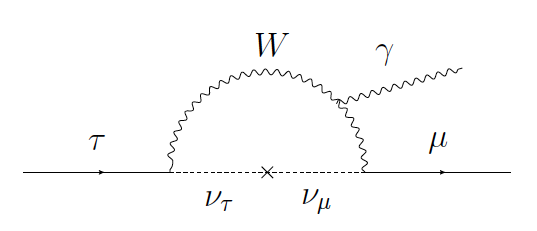
\includegraphics[width=\textwidth]{images/tauMG-feynman.png}
            \caption[Network2]%
            {{\small}}    
            \label{fig:mean and std of net14}
        \end{subfigure}
        \hfill
        \begin{subfigure}[b]{0.475\textwidth}  
            \centering 
            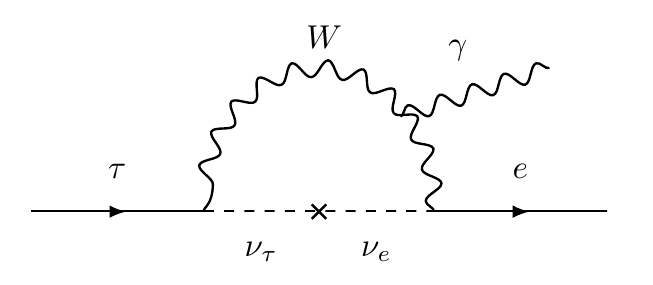
\includegraphics[width=\textwidth]{images/tauEG-feynman.png}
            \caption[]%
            {{\small}}    
            \label{fig:mean and std of net24}
        \end{subfigure}
        \caption{Feynman diagrams for (a) $\tau\to\mu\gamma$ and (b) $\tau\to e\gamma$ proceeding through SM processes.}
    \end{figure}

LFV necessarily requires generation mixing between leptons to occur. Though this is prohibited in the Standard Model, the discovery of neutrino oscillations proves that flavour mixing does occur in our universe; that is, flavour is not conserved. We seek to discover whether this LFV can be observed in other areas of flavour physics.

In the Standard Model + massive neutrinos, the only source of LFV is from the operators responsible for neutrino mass. However, the relevant Feynman diagrams (see Figure) are ``loop suppressed'' and proportional to the GIM factor, given as $\left(\frac{m_\nu}{M_W}\right)^4$; as neutrino mass is very small ($\mathcal{O}(\SI{0.3}{eV})$) we expect the LFV effects to be negligible! With these operators the branching ratio for, say, $\tmg$ is $\sim 10^{-40}$ \cite{Passemar:2015}. With such little SM background, observation of an LFV process of the type $\tlg$ would be an unambiguous signature of NP.

\begin{equation}
\mathcal{B}(\tau\to\ell\gamma)=\frac{3\alpha}{32\pi}\lvert U^{\star}_{\tau i} U_{\mu i}\frac{\Delta^2_{3i}}{m_W^2}\rvert^2
\leq 10^{-53}\sim 10^{-49}
\end{equation}


\section{Other LFV}

In many NP models, LFV is not limited to just $\tlg$ decays. There have been searches for other LFV modes, such as $\mu\to e \gamma$, and $\tau\to 3\ell$. Current limits on the branching fractions are given in Figure \ref{tab:current lfv bounds} below \cite{Paradisi:2016}.

\begin{table}[h]
\centering
\label{my-label}
\begin{tabular}{lll}
\textbf{LFV process} & \textbf{Present bound} & \textbf{Future sensitivity} \\ \hline
$\mu\to e\gamma$ & \num{5.7e-13} & $\approx\num{6e-14}$ \\
$\mu\to 3e$ & \num{1.0e-12} & $\approx\num{e-16}$ \\
$\tau\to e\gamma$ & \num{3.3e-9} & $\sim\num{e-8} - \num{e-9}$ \\
$\tau\to\mu\gamma$ & \num{4.4e-9} & $\sim\num{e-8} - \num{e-9}$ \\
$\tau\to 3e$ & \num{2.7e-8} & $\sim\num{e-9} - \num{e-10}$ \\
$\tau\to 3\mu$ & \num{2.1e-8} & $\sim\num{e-9} - \num{e-10}$
\end{tabular}
\caption{Current experimental limits on various LFV processes}
\label{tab:current lfv bounds}
\end{table}

Moving into future sensitivities accessible from experiments such as Belle II, we see that the upper limits of branching fractions for $\tlg$ decays could be improved by $1-2$ orders of magnitude!

\section{Hints of LFV beyond the Standard Model}

Motivations behind the search for LFV come from both theoretical and experimental results. The primary experimental motivations is the existence of neutrino mixing, though anomalous results such as the $\htm$ excess observed at CMS in 2015 also hint at LFV beyond the Standard Model. On the theoretical side, LFV is predicted in a variety of NP models. In fact, many models which introduce mechanisms to generate neutrino mass also inadvertantly allow LFV in other sectors of non-negligible order! We shall discuss these motivations below.


\subsection{Neutrino mixing}

The discovery that flavour mixing can occur in the neutrino sector \cite{SuperK:1998}\cite{SNO:2002} proves that neutrinos have mass. Both the concept of massive neutrinos, and by extension the mechanisms which generate neutrino mass, are not predicted or explained by the SM. This tells us that the lepton sector is not fully understood.

There are many NP models which introduce mechanisms to give neutrinos mass. These include SUSY, seesaw models, and many others. In introducing these mechanisms, many of these models inadvertently introduce LFV! As a particle example, a Type-II seesaw model posits a scalar triplet of Higgs-like particles \cite{Passemar:2015}. This triplet comprises a doubly-charged Higgs, a singly-charged Higgs, and a neutral Higgs. As show in Figure X below, lepton-flavour violating processes could proceed via leptons coupling to these scalars!


\begin{figure}[h]
\centering
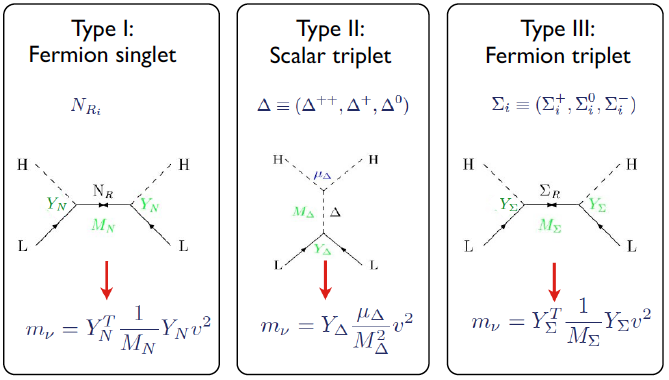
\includegraphics[width=0.7\textwidth]{images/seesaw.png}
\caption{New particles introduced in seesaw models (Passemar, 2015)}
\label{}
\end{figure}

\begin{figure}[h]
\centering
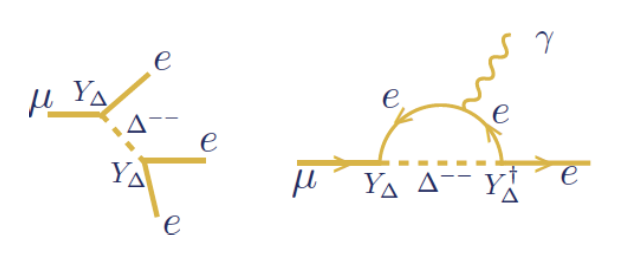
\includegraphics[width=0.5\textwidth]{images/seesaw-lfv-modes.png}
\caption{Scalars introduced in Type-II seesaw models mediating LFV decays (Passemar, 2015)}
\label{}
\end{figure}

\subsection{$\htm$ excess}

Hints of LFV can come in the form of experimental results which are not consistent with the SM. One such ``anomaly’’ is the $\htm$ excess. In 2015, CMS found a $2.4\sigma$ excess in the branching fraction of $\htm$ \cite{CMS:2015a}. This process is lepton flavour violating, so in the SM its branching fraction is expected to be consistent with zero. However it was determined

\begin{equation}
\br(h\to \tau \mu) = (0.84^{+0.39}_{-0.37})\%
\end{equation}

Also in 2015 was a similar search performed by ATLAS \cite{ATLAS:2015}, in which an excess of $1.2\sigma$ was found in the $\htm$ decay. 

\begin{equation}
B(\htm) = (0.77 \pm 0.66)\%
\end{equation}

Though this $1.2\sigma$ result is less indicative of NP, it still provides hints as to where NP could occur. These results indicate possible new physics in the Higgs sector! Several models, including Two-Higgs Doublet Models (2HDM), introduce new Higgs-like particles; these particles can couple with leptons to allow lepton flavour violating processes \cite{Harnik:2012}. In fact, LFV can occur naturally in any model with more than one Higgs doublet.

\begin{figure}[h]
\centering
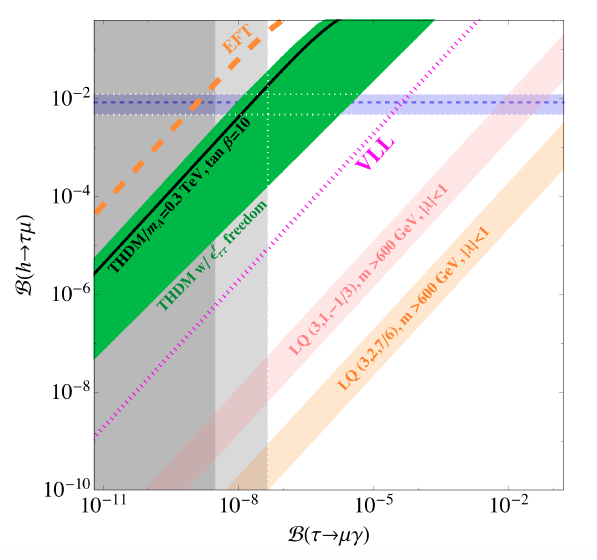
\includegraphics[width=0.7\textwidth]{images/h-vs-tau.png}
\caption{Correlation between $\br(\htm)$ and $\br(\tmg)$ in various NP scenarios (Dorsner et al., 2015)}
\label{}
\end{figure}

The present experimental result for $\br(\htm)$ is shown in horizontal blue band; current and future projections for $\br(\tmg)$ experimental sensitivity are represented with vertical light and dark gray bands. We note that certain 2HDM models predict a branching fraction for $\br(\tmg)$, consistent with the CMS results, at sensitivities which could be observed by Belle II. It is important to note that the Higgs sector could contribute to LFV in NP scenarios, and that both theory and experimental limits on other LFV processes such as $\htm$ all interweave with limits on $\tlg$ branching fractions to provide information on NP, even just through reducing the available phase space for certain models \cite{Dorsner:2015}.

\begin{figure}[h]
\centering
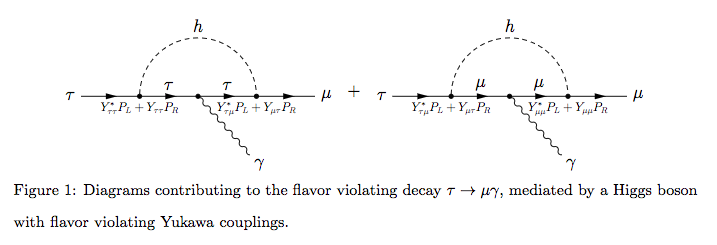
\includegraphics[width=0.9\textwidth]{images/higgs-lfv-modes.png}
\caption{Diagrams contributing to $\tmg$ decay, mediated by a Higgs boson with flavour violating Yukawa coupling (Harnick et al., 2012)}
\label{}
\end{figure}

As seen in Figure above, new Higgs particles can mediate LFV processes and allow for measurable amounts of LFV beyond the Standard Model \cite{Dorsner:2015}.


\subsection{Models predicting $\tlg$}

As mentioned previously, LFV in the $\tau$ sector is introduced in many NP scenarios as a consequence of generating neutrino mass (and hence facilitating neutrino mixing). Branching fractions of the modes $\tlg$ are highly calculable - there is little theoretical uncertainty.

\begin{figure}[h]
\centering
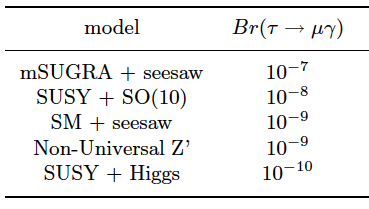
\includegraphics[width=0.5\textwidth]{images/np-models-bounds.png}
\caption{Upper limits of branching fractions from $\tmg$, predicted by models of new physics beyond the SM (various sources)\cite{Ohshima:2007zz}}
\label{}
\end{figure}

Figure above lists a few NP models with their predictions of $\br(\tmg)$. We see that the phase space of some of these models has already been ruled out with our current experimental limits on LFV branching fractions.


\section{Past searches for $\tlg$}

The most recent searches for $\tlg$ were undertaken at Belle (2007) and Babar (2010), for both $\ell=\mu,e$ modes. These detectors are $e^+ e^-$ colliders a signal of the form $e^+ e^-\to \tau^+ \tau^-$, with one tau (signal-side) decaying $\tau\to \ell \gamma$ and the other tau (tag-side) decaying generically, with the requirement that the tag-side track is not $\ell$.


\subsection{Belle searches}


   \begin{figure}[h]
        \centering
        \begin{subfigure}[b]{0.475\textwidth}
            \centering
            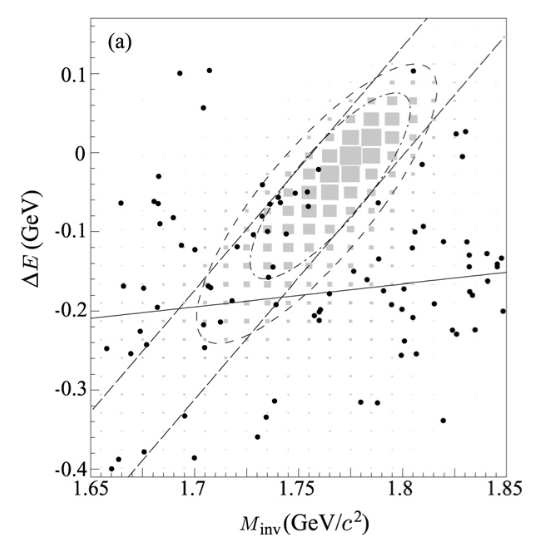
\includegraphics[width=\textwidth]{images/belle-search-tauMG-signal-region.png}
            \caption[Network2]%
            {{\small}}    
            \label{fig:mean and std of net14}
        \end{subfigure}
        \hfill
        \begin{subfigure}[b]{0.475\textwidth}  
            \centering 
            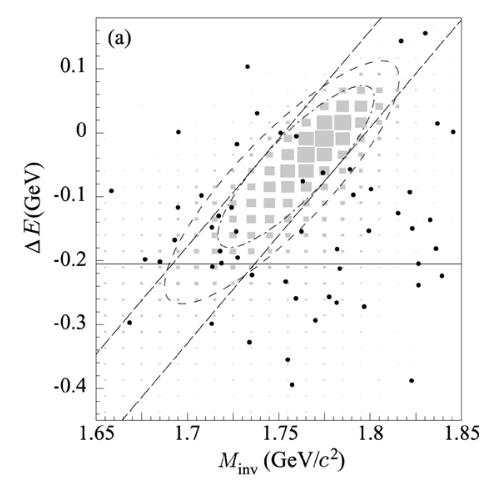
\includegraphics[width=\textwidth]{images/belle-search-tauEG-signal-region.png}
            \caption[]%
            {{\small}}    
            \label{fig:mean and std of net24}
        \end{subfigure}
        \caption{$M_{\text{inv}}$-$\Delta E$ distribution in the search for (a) $\tau\to\mu\gamma$ and (b) $\tau\to e\gamma$ at Belle over a $\SI{515}{fb^{-1}}$ data set. $M_{\text{inv}}$ is the reconstructed mass of the $\tau$ from these processes, $\Delta E$ is the energy difference between this reconstructed $\tau$ and half center-of-mass frame beam energy. Dots are the data and shaded boxes indicate the signal MC. The dashed ellipse shows the $3\sigma$ region and the dot-dashed ellipse is the $2\sigma$ signal region.}
    \end{figure}


The Belle detector records events from an asymmetric $e^+ e^-$ collider with electron (positron) energy of $\SI{8}{GeV}$ ($\SI{3.5}{GeV}$). A detailed discussion of the detector can be found at Ref. \cite{Belle:2002}. In 2007, the Belle Collaboration performed a search over $\SI{535}{fb^{-1}}$ of $e^+ e^-$ data and set constraints \cite{Hayasaka:2007} on $\tlg$ branching fractions as

\begin{align*}
\br(\tmg)&<\num{4.5d-8},\\
\br(\tau\to e \gamma)&<\num{1.2d-7}.
\end{align*}



\subsection{Babar searches}

   \begin{figure}[h]
        \centering
        \begin{subfigure}[b]{0.475\textwidth}
            \centering
            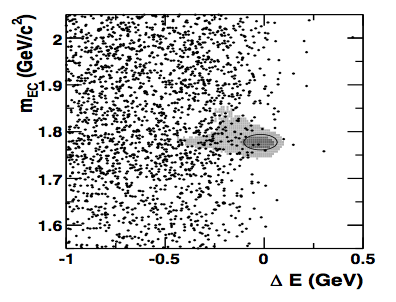
\includegraphics[width=\textwidth]{images/babar-search-tauMG-signal-region.png}
            \caption[Network2]%
            {{\small}}    
            \label{fig:mean and std of net14}
        \end{subfigure}
        \hfill
        \begin{subfigure}[b]{0.475\textwidth}  
            \centering 
            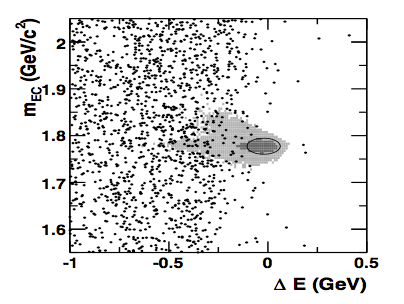
\includegraphics[width=\textwidth]{images/babar-search-tauEG-signal-region.png}
            \caption[]%
            {{\small}}    
            \label{fig:mean and std of net24}
        \end{subfigure}
        \caption{$M_{\text{bc}}$-$\Delta E$ distribution in the search for (a) $\tau\to\mu\gamma$ and (b) $\tau\to e\gamma$ at Babar over a $\SI{515}{fb^{-1}}$ data set. $M_{\text{bc}}$ is the beam-constrained mass of the $\tau$ from these processes, $\Delta E$ is the energy difference between this reconstructed $\tau$ and half center-of-mass frame beam energy. Data are shown as dots and contours containing \num{90}{\percent} (\num{50}{\percent}) of signal MC events are shown as light- (dark-) shaded regions.}
    \end{figure}


Similar to Belle, the Babar detector records events from an asymmetric $e^+e^-$ collider, with electron (positron) energy of $\SI{9}{GeV}$ ($\SI{3.1}{GeV}$). A detailed discussion of the detector can be found at Ref. \cite{Babar:2002}. The most recent search for $\tlg$ was performed in 2010 by the Babar Collaboration \cite{Babar:2010}, over a $\SI{515.5}{fb^{-1}}$ dataset, setting constraints on $\tlg$ branching fractions as

\begin{align*}
\br(\tmg)&<\num{4.4d-8},\\
\br(\tau\to e \gamma)&<\num{3.3d-8}.
\end{align*}


\section{The role of this analysis (rephrase plz)}

Collection of data at Belle II is scheduled to begin in 2017. A physics program has been designed for the experiment, detailing specific decays to investigate and areas of particle physics to probe. It is important before data collection begins to perform sensitivity studies on these decay processes, to find areas in which the analysis performs better or worse than expected. In some cases we may find that background rejection is greater than previously modelled due to, for example, good performance in particle identification by the detector. It is also important if areas for improvement are found, such as beam background degrading analysis performance. Finding areas for improvement during the development stage informs future development, including tracking and reconstruction software and hardware-based beam background mitigation techniques, and leads to more optimal conditions for physics events to be investigated.


This analysis is the first $\tau$ physics study for Belle II. Some key points studied are muon and electron track reconstruction and the effects of beam background on XXXXX (???). Information on these areas of event analysis is not only useful for $\tau\to\ell\gamma$ searches at Belle II --- the physics program for the experiment includes a range of $\tau$ decay processes (see Table XXX) of which many require muon and electron track reconstruction. Low-multiplicity events require XXXXXX, so XXXXXX.

\begin{table}[h]
\centering
\label{my-label}
\begin{tabular}{lll}
\textbf{LFV process} & \textbf{Present bound} & \textbf{Future sensitivity} \\ \hline
$\tau\to e\gamma$ & \num{3.3e-9} & $\sim\num{e-8} - \num{e-9}$ \\
$\tau\to\mu\gamma$ & \num{4.4e-9} & $\sim\num{e-8} - \num{e-9}$ \\
$\tau^{\pm}\to e^{\pm} e^{\mp} e^{\pm}$ & \num{2.7e-8} & $\sim\num{e-9} - \num{e-10}$ \\
$\tau^{\pm}\to \mu^{\pm} \mu^{\mp} \mu^{\pm}$ & \num{2.1e-8} & $\sim\num{e-9} - \num{e-10}$
\end{tabular}
\caption{Current experimental limits on various LFV processes}
\label{tab:current lfv bounds}
\end{table}

Results from this analysis will be published in the Belle II physics book, which is currently being compiled by members across all working groups in the collaboration. The book aims to (????); this study will provide the basis for future $\tau$ LFV studies at Belle II. This study also validates the projected increase in sensitivity for $\tau\to\ell\gamma$ branching fractions from Belle to Belle II.

\begin{figure}[h]
\centering
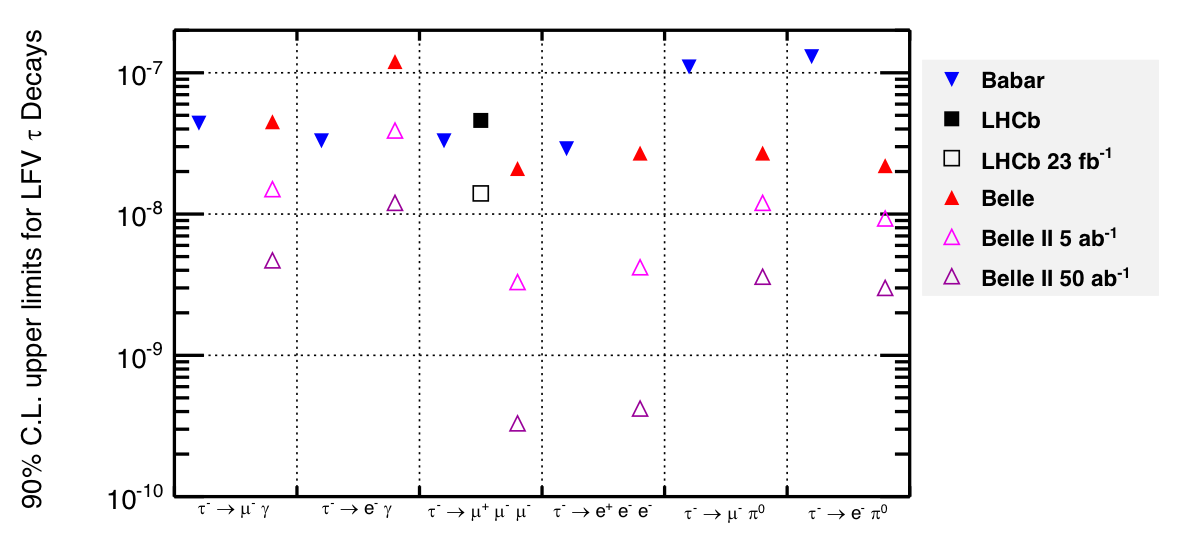
\includegraphics[width=0.9\linewidth]{images/current-future-sensitivities.png}
\caption{Current and future sensitivities on $\tau$ LFV branching fractions (\emph{Urquijo}, 2016). \textbf{NOTE: remove the unrelated LFVs}}
\label{}
\end{figure}

%-------------------------------------------------------------------

\chapter{The Belle and Belle II detectors}

Located in Tsukuba, Japan, the KEKB particle accelerator was used for the Belle experiment from 1999 to 2010 and collided high energy electrons and positrons of $\SI{8}{GeV}$ and $\SI{3.5}{GeV}$ respectively. This experiment made important discoveries on the flavour structure of elementary particles, notably in the quark section where CP symmetry violation was discovered. Efforts by the Belle Collaboration culminated in the 2008 Nobel Prize awarded to Makoto Kobayashi and Toshihide Maskawa for their theory of CP violation. Over its lifetime, the Belle detector collected a total time-integrated luminosity of $\SI{1000}{fb^{-1}}$, corresponding to ???? tau-pair events. An upgrade to the KEKB collider known as SuperKEKB is expected to be complete by 2014 \textbf{(LOL)} as part of the Belle II experiement.

\begin{figure}[h]
\centering
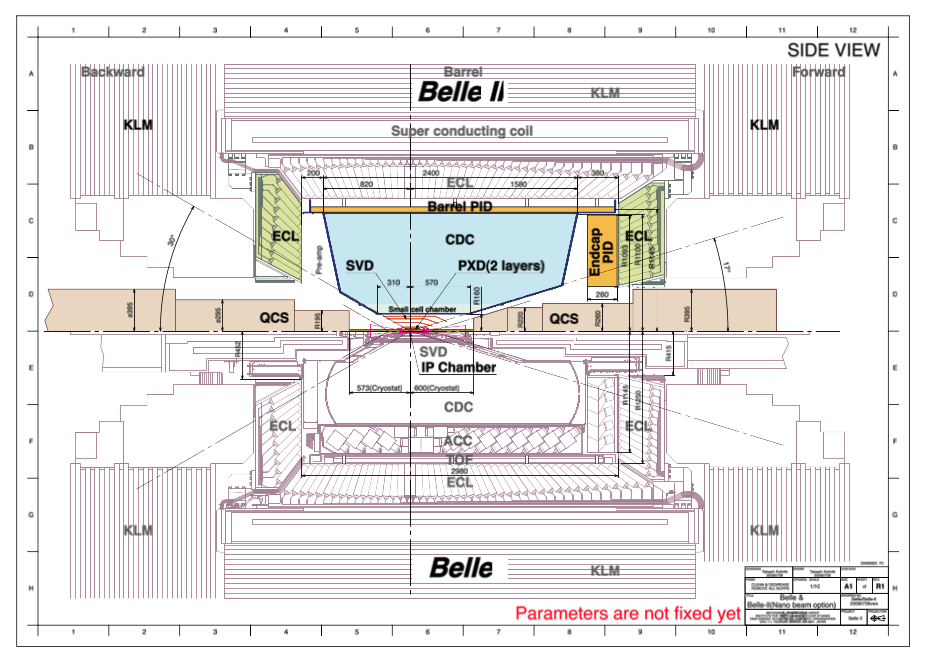
\includegraphics[width=0.7\linewidth]{images/super-kekb-side-view.png}
\caption{Super-KEKB detector design, side-view}
\label{}
\end{figure}

Over the course of the experiment, it is projected that Belle II will collect a total time-integrated luminosity of $\SI{50}{ab^{-1}}$. This is a much larger data sample than the $\SI{1}{ab^{-1}}$ collected at Belle. Electron-positron beam energies differ from those used at Belle, with high-energy-ring (HER) electron beam energy of $\SI{7}{GeV}$ and low-energy-ring (LER) positron beam energy  of $\SI{4}{GeV}$. Design luminosity in the detector is increased by 40 over Belle; this increases background hit rate (???) by a factor of 20, while physics event rate is expected to be 50 times higher than at Belle.

Key components of the detector are the silicon vertex detector (SVD), the central drift chamber (CDC), the electromagnetic calorimeter (ECL), the time-of-flight/Cerenkov aerogel chamber (TOP), and the K-long/muon detector (KLM). Many of these will be upgraded in Belle II to provide better performance; in some cases the full reconstruction software is rewritten even when the hardware is not improved.

%-------------------------------------------------------------------

\section{Pixel Detector}


%-------------------------------------------------------------------

\section{Silicon Vertex Detector}


%-------------------------------------------------------------------


\section{Central Drift Chamber}

Smaller drift cells than Belle; extends to a large radius.

%-------------------------------------------------------------------


\section{Electromagnetic Calorimeter}

Possible replacement of endcap scintillator crystral with a faster and radiation tolerant version.

New electronics of ECL considerably reduce noise pile-up.
`
I can talk about the importance of cluster timing

\url{https://docs.belle2.org/record/344/files/BELLE2-NOTE-TE-2016-006.pdf}

%-------------------------------------------------------------------


\section{Time-of-flight/Cerenkov aerogel chamber}

%-------------------------------------------------------------------

\section{K-long/muon detector}

%-------------------------------------------------------------------

\section{Particle identification (PID)}

These PID values are generated through combination of many components of the detector, and provide the probability of a track being a particular particle. Some tracks may be double counted or misreconstructed. To account for this, several tighter PID cuts are implemented later.

%-------------------------------------------------------------------

\section{Beam backgrounds}

SEE TECHNICAL DESIGN REPORT

Beam background is an important issue in B-factories, and especially so for the upgraded energies of SuperKEKB. Key sources of this beam background are synchrotron radiation (SR), beam-gas scattering, and Touschek radiation.

Scattered particles and radiation photons generated by these processes collide with the beam pipe and generate showers of photons, leptons and hadrons. Additionally, other particles can be generated at the interaction point of the collision between opposite beams; these are mostly electron-positron pairs. These particles then interact with the detector, and are called beam background. This background can make searches for interesting physics events difficult, due to the large number of clusters and tracks introduced.

\subsection{Synchrotron radiation}

As beam particles are bent by magnets while travelling through the accelerator, they emit synchrotron radiation.

\subsection{Beam-gas scattering}	

The region inside the beam pipe is not a perfect vacuum; the designed gas pressure for SuperKEKB is $\SI{e-7}{Pa}$. Most of this gas is composed of neutral H$_2$ and CO$_2$. Beam particles can collide with the gas molecules, resulting in elastic scattering where energy is unchanged but direction is changed (Coulomb scattering), or inelastic scattering whereby a photon is emitted from the scattered particle (bremsstrahlung).

  \begin{figure}[h]
        \centering
        \begin{subfigure}[b]{0.475\textwidth}
            \centering
            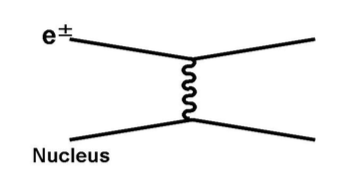
\includegraphics[width=\textwidth]{images/coulomb-scattering.png}
            \caption[Network2]%
            {{\small Coulomb scattering}}    
            \label{fig:mean and std of net14}
        \end{subfigure}
        \hfill
        \begin{subfigure}[b]{0.475\textwidth}  
            \centering 
            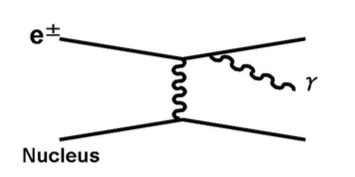
\includegraphics[width=\textwidth]{images/bremsstrahlung.png}
            \caption[]%
            {{\small Bremsstrahlung}}    
            \label{fig:mean and std of net24}
        \end{subfigure}
    \end{figure}


\subsubsection{Coulomb scattering}

Beam electrons and positrons can elastically scatter off beam gas particles, changing direction such that the scattered particle does not reach the interaction point.

\subsubsection{Bremsstrahlung}

Beam-gas scattering can also occur as bremsstrahlung, where electrons (or positrons) recoil off gas nuclei and emit photons (see figure XXXX b) above). The photon carries away for fraction of the scattered particle's energy.


\subsection{Touschek scattering}

Particle beams do not exist as continuous ``lines'' of electrons and positrons marching through the accelerator in single file. Instead, we have tightly packed beam bunches, containing $10^{10} - 10^{11}$ particles each. In Super-KEKB the bunches have a designed cross-section perpendicular to the beam trajectory of XXXXX, up from XXXXX in KEKB (LENGTH??). These bunches are aligned almost perfectly parallel so that beam particles do not collide with the beam pipe during their many cycles around the accelerator.

Within these bunches the particles oscillate in a direction perpendicular to the beam trajectory, so that in addition to interacting with beam-gas, particles within a beam bunch collide with each other resulting in an transfer of energy and momentum. Trajectories of these particles may be changed by this interaction, so that they do not reach the interaction point. 

\begin{figure}[h]
\centering
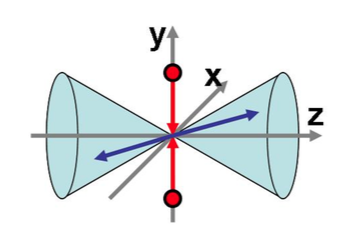
\includegraphics[width=0.5\linewidth]{images/touschek-beam-frame.png}
\caption{An illustration of Touschek scattering in the bunch frame}
\label{fig:test2}
\end{figure}



%-------------------------------------------------------------------

\chapter{Monte Carlo production and background types}

Electron-positron collisions at Belle II will produce a wide range of different physics events. Within these, we hope to find the signal modes $\tau\to\mu\gamma$ and $\tau\to e\gamma$. Many other events, known as ``background'' events, will.....

In this analysis, we investigate all generically decaying tau-pair processes, mu-pair events ($e^+ e^- \to \mu^+ \mu^- (\gamma)$), bhabha scattering ($e^+ e^- \to e^+ e^- \gamma$), qqbar continuum (where $q = u, d, c, s$), and generic B$\bar{\text{B}}$ continuum ($e^+ e^- \to B^+ B^-$ and $e^+ e^- \to B^0 \bar{B}^0$). Of the tau-pair processes, we specifically investigate the modes $\tau^{\pm} \to \mu^{\pm} \nu \nu$, $\tau^{\pm} \to e^{\pm} \nu \nu$, and $\tau^{\pm} \to \pi^{\pm} \nu$, as these are expected to be dominant backgrounds.

We investigate the characteristic signals of observables such as momentum, energy, and polar angles (object trajectory relative to collision axis ???) as well as other constructed variables, in simulated data known as Monte Carlo (MC). By looking at signal and background signals separately in MC, we are able discriminate between signal and background events in data (NO I don't actually do this.... feasibility test? Not sure how to describe why I do what I do and what it accomplishes).

\section{Physics backgrounds}

The dominant backgrounds for the process $\tmg$ are $\tau\to \mu \nu \nu$, $\tau\to \pi \nu$ and $e^+ e^- \to \mu^+ \mu^- \gamma$ (with similar backgrounds for $\tau\to e \gamma$) \cite{Hayasaka:2007}. The first two backgrounds have branching fractions
\begin{align*}
\br(\tau\to \mu \nu \nu)&=\num{17.41}{\percent},\\
\br(\tau\to\pi\nu)&=\num{10.83}{\percent},
\end{align*}
which are non-negligible contributions to the dataset. The cross-section for we can compare the cross section of $e^+ e^- \to \mu^+ \mu^- \gamma$ to that of $e^+ e^- \to \tau^+ \tau^- \gamma$;
\begin{align*}
\sigma(e^+ e^- \to \mu^+ \mu^- \gamma)&=\SI{0.242}{nb},\\
\sigma(e^+ e^- \to \tau^+ \tau^- \gamma)&=\SI{0.919}{nb},\\
\end{align*}
so we note a significant contribution from this background also.

  \begin{figure}[h]
        \centering
        \begin{subfigure}[b]{0.315\textwidth}
            \centering
            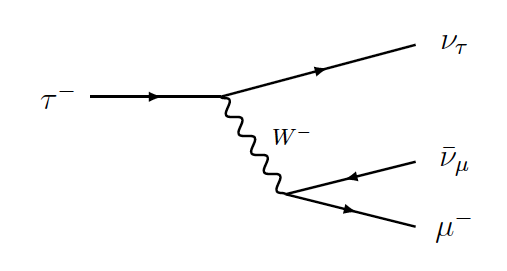
\includegraphics[width=\textwidth]{images/taumununu.png}
            \caption[Network2]%
            {{\small $\tau\to \mu \nu \nu$}}    
            \label{fig:mean and std of net14}
        \end{subfigure}
        \hfill
        \begin{subfigure}[b]{0.315\textwidth}  
            \centering 
            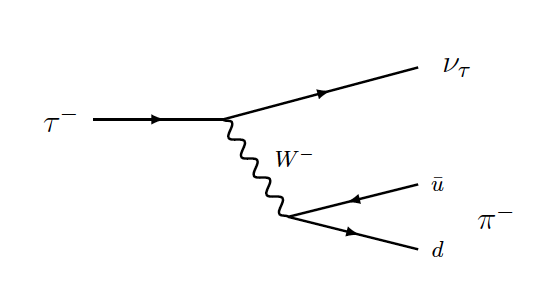
\includegraphics[width=\textwidth]{images/taupinu.png}
            \caption[]%
            {{\small $\tau\to \pi \nu$}}    
            \label{fig:mean and std of net24}
        \end{subfigure}
                \hfill
        \begin{subfigure}[b]{0.315\textwidth}  
            \centering 
            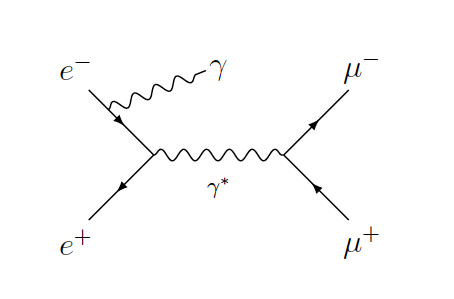
\includegraphics[width=\textwidth]{images/eemumugamma.png}
            \caption[]%	
            {{\small $e^+ e^- \to \mu \mu (\gamma)$}}    
            \label{fig:mean and std of net24}
        \end{subfigure}
        \caption{Feynman diagrams for the dominant physics backgrounds for $\tmg$.}
    \end{figure}


\section{Event generation}

All MC was generated in the Belle II Analysis Framework (\texttt{basf2}) with geometry and energies from SuperKEKB. HOW DOES GENERATION HAPPEN? 

Geometry information of the detector includes very specific location, thickness and material values; magnetic field strength through the detector is also known. The detector components are simulated by the generator, so that timing information and energy deposition is recorded for these components as MC particles interact with them. Following the simulation of a physics event, information from the sub-detectors is used to reconstruct tracks (correponding to charged particles) and clusters (referring to cells of the ECL with which a particle has interacted with, corresponding to photons).

\subsection{Signal generation}

Signal MC was produced using the \texttt{KKMC} generator (REF PHILL'S GENERATOR PAPER). Decays proceeded as $e^+ e^- \to \tau^+ \tau^-$, with one tau decaying to the signal mode $\tau \to \ell \gamma$ (the signal-side), and the other (the tag-side) decaying to all experimentally measured SM decay modes of the tau, scaled by their branching ratio; decaying according to the SM is referred to generic decay. The modes $\tau^+ \to \ell^+ \gamma$, $\tau^-$ decaying generically, and $\tau^- \to \ell^- \gamma$, $\tau^+$ decaying generically were both generated so that differences were not overlooked. To investigate both the electron and muon modes, two distinct final states were produced. The number of produced events was 3,100,000 for the muon final state, and 3,550,000 for the electron final state.

The \texttt{KKMC} generator


\subsection{Background generation}

Samples for a range of background events were produced by the Belle II Collaboration. 

Continuum = KKMC ($e^+e^-\to q\bar{q}$, PYTHIA8.2 ($q\bar{q}\to\text{hadrons}$) and EvtGen (decay of unstable hadrons). These generators were not used to produce $q\bar{q}$ pairs at Belle.


\section{Event scaling}

The full Belle II dataset is expected to have a time-integrated luminosity of $\SI{50}{ab^{-1}}$ (UM HMM what do I do here). Instead of running over the equivalent amount of background events expected in such a sample size, we can run over a smaller number of events then scale our results. This is done for computing reasons, as the number of background events recorded for these luminosities quickly becomes prohibitively large.

We choose to scale up to a luminosity of $\SI{1}{ab^{-1}}$; this is the total time-integrated luminosity of the complete Belle dataset, and so is useful as a point of comparison to previous searches. The scale factor for each event type is calculated by

\begin{equation}
n_{\SI{1}{ab^{-1}}} = n_{\text{generated}} \times \text{scale factor},
\end{equation}

where $n_{\SI{1}{ab^{-1}}}$ = $\mathcal{L} \sigma$, and $n_{\text{generated}}$ is the number of events generated. Scaled event numbers are presented in Table XXXX below.

\begin{table}[h]
\centering
\begin{tabular}{lrrr}
\textbf{Event type} & $\mathbf{n_{\text{generated}}}$ & \textbf{scale factor} & $\mathbf{n_{\SI{1}{ab^{-1}}}}$ \\ \hline
\rowcolor[HTML]{EFEFEF} 
$\tau \to \mu\gamma$ & \num{3200000} & \num{2.58e-05} & \num{83} \\
\rowcolor[HTML]{EFEFEF}
$\tau \to e\gamma$ & \num{2550000} & \num{8.65E-05} & \num{221} \\       
$\tau \to \mu\nu\nu$ & \num{127998320} & \num{1.250} & \num{159997900} \\
$\tau \to \pi\nu$ & \num{267245200} & \num{1.250} & \num{334056500}  \\
$\tau \to e\nu\nu$ & \num{131086160} & \num{1.250} & \num{163857700}  \\
$\tau \to \text{generic}$ & \num{208870320} & \num{1.250} & \num{261087900} \\
$e^+e^- \to \mu^+\mu^-(\gamma)$ & \num{148600000} & \num{7.725} & \num{1148000000}  \\
$e^+e^- \to e^+e^-(\gamma)$ & \num{15630000} & \num{19193.858} & \num{300000000000}  \\
$e^+e^- \to u\bar{u}$ & \num{1268991935} & \num{1.269} & \num{1610000000} \\
$e^+e^- \to d\bar{d}$ & \num{317048262} & \num{1.262} & \num{400000000} \\
$e^+e^- \to c\bar{c}$ & \num{1039855756} & \num{1.250}  & \num{1300000000} \\
$e^+e^- \to s\bar{s}$ & \num{289900586} & \num{1.310}  & \num{380000000}  \\
$e^+e^- \to B^+B^-$ & \num{451320000} & \num{1.219}  & \num{550000000}  \\
$e^+e^- \to B^0\bar{B}^0$ & \num{427680000} & \num{1.286}  & \num{550000000} 
\end{tabular}
\caption{Scaled event numbers}
\label{my-label}
\end{table}

Unless explicitly stated, scaled event numbers will be used throughout this report (??? paper/thesis/document/analysis??) as to provide accurate points of comparison between events.


\section{Version differences}

The software framework on which event generation was performed is undergoing continuous development; a majority of signal and background MC was produced on the same release version to ensure accuracy between MC types. This version was made available on XXXXX, and was one of the most up-to-date releases at the time of analysis. However, the backgrounds $\mu^+\mu^-(\gamma)$ and $e^+ e^-(\gamma)$ (mu-pair and bhabha, respectively) did not have any events generated using this release, and instead used an older release dated XXXXX.

A full investigation into the differences in generated MC between releases has not been performed in this analysis, as it is assumed they are negligible in most relevant cases. Changes relate mostly to generation of beam backgrounds (??); however one major change is in the reporting of timing data from the ECL. From the release dated XXXX onwards, these associated times will be reported in nanoseconds, rather than uncalibrated clock ticks (REF). In comparing samples of background MC generated in both the older and newer releases, figures XXXX a) and b) below, as well as private correspondance with the developer responsible for these changes, it was found that conversion to the newer scale could be made by adding 80 units to the cluster timing values.

   \begin{figure}[h]
        \centering
        \begin{subfigure}[b]{0.475\textwidth}
            \centering
            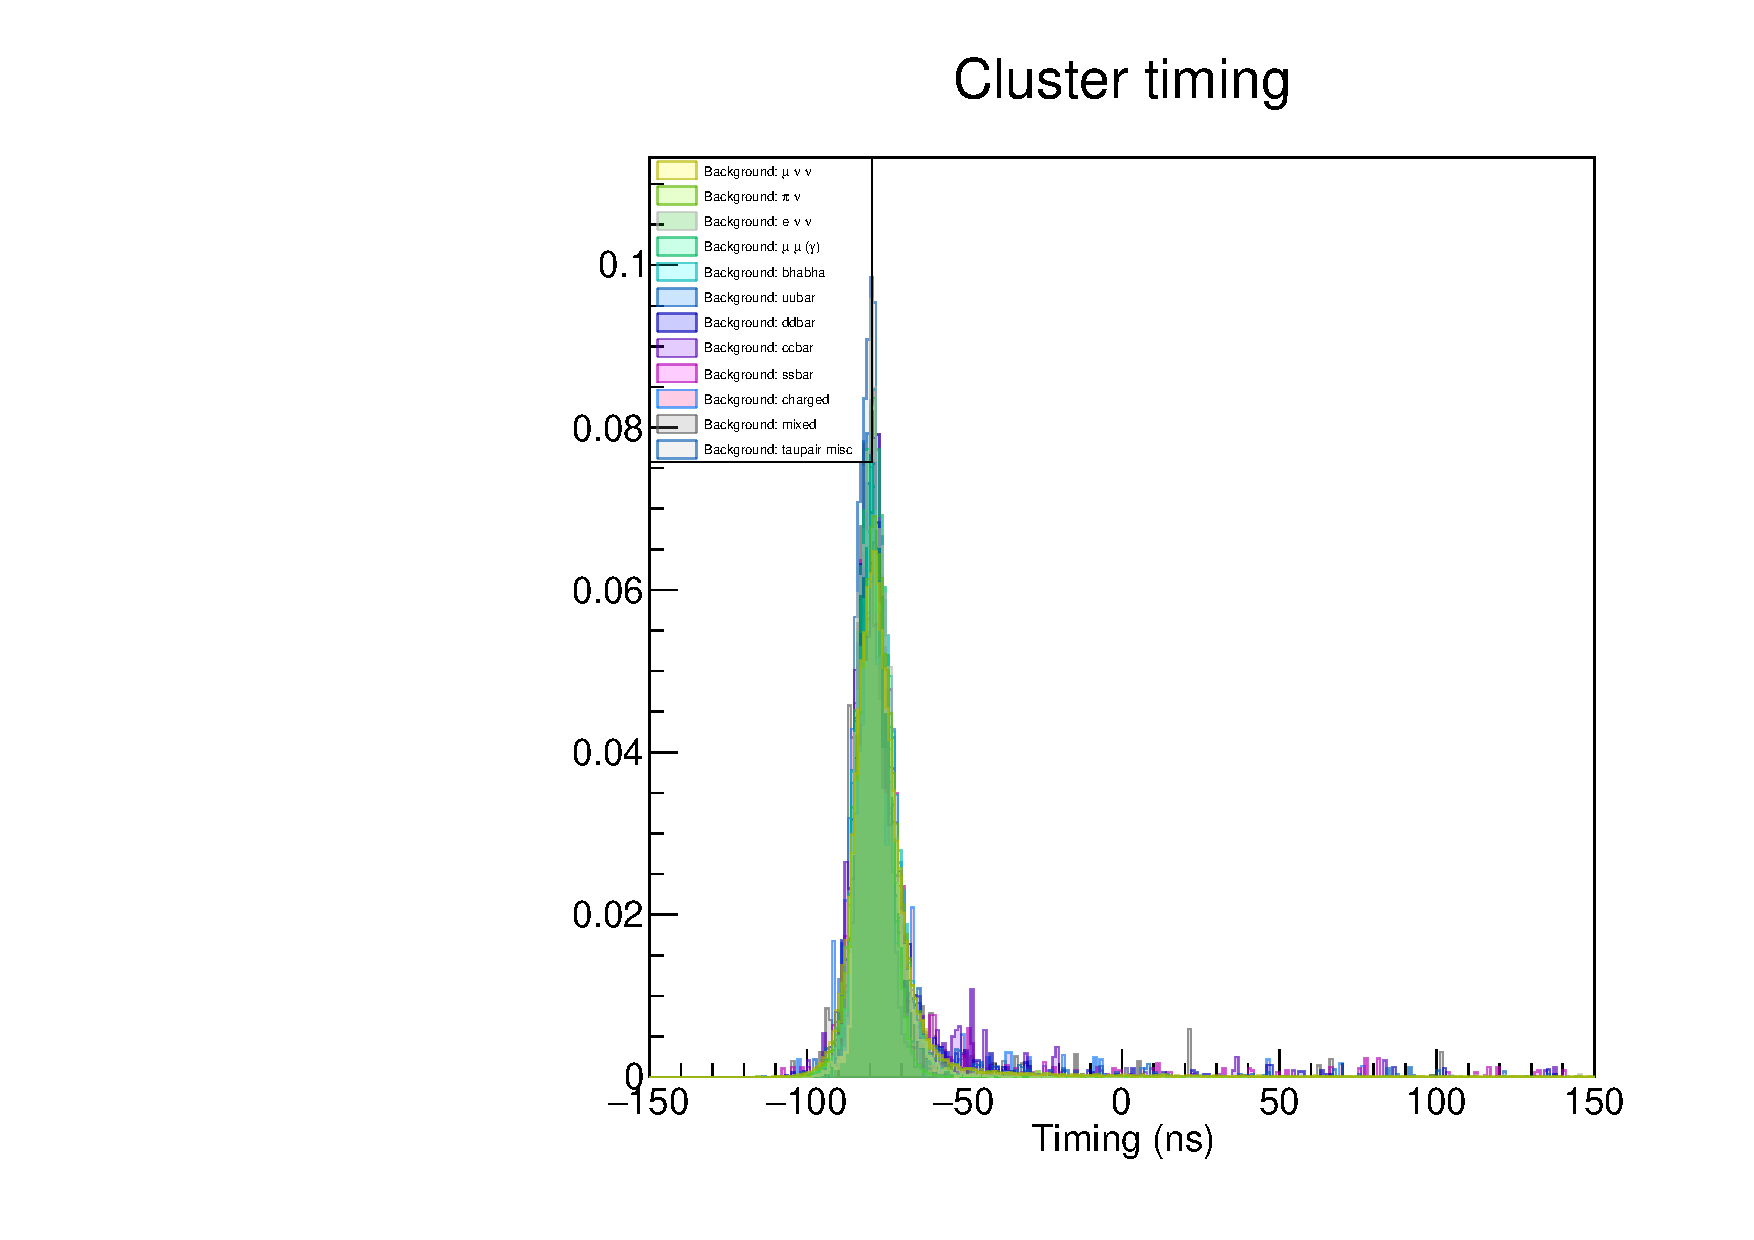
\includegraphics[width=\textwidth]{images/cluster-timing-old.pdf}
            \caption[Network2]%
            {{\small}}    
            \label{fig:mean and std of net14}
        \end{subfigure}
        \hfill
        \begin{subfigure}[b]{0.475\textwidth}  
            \centering 
            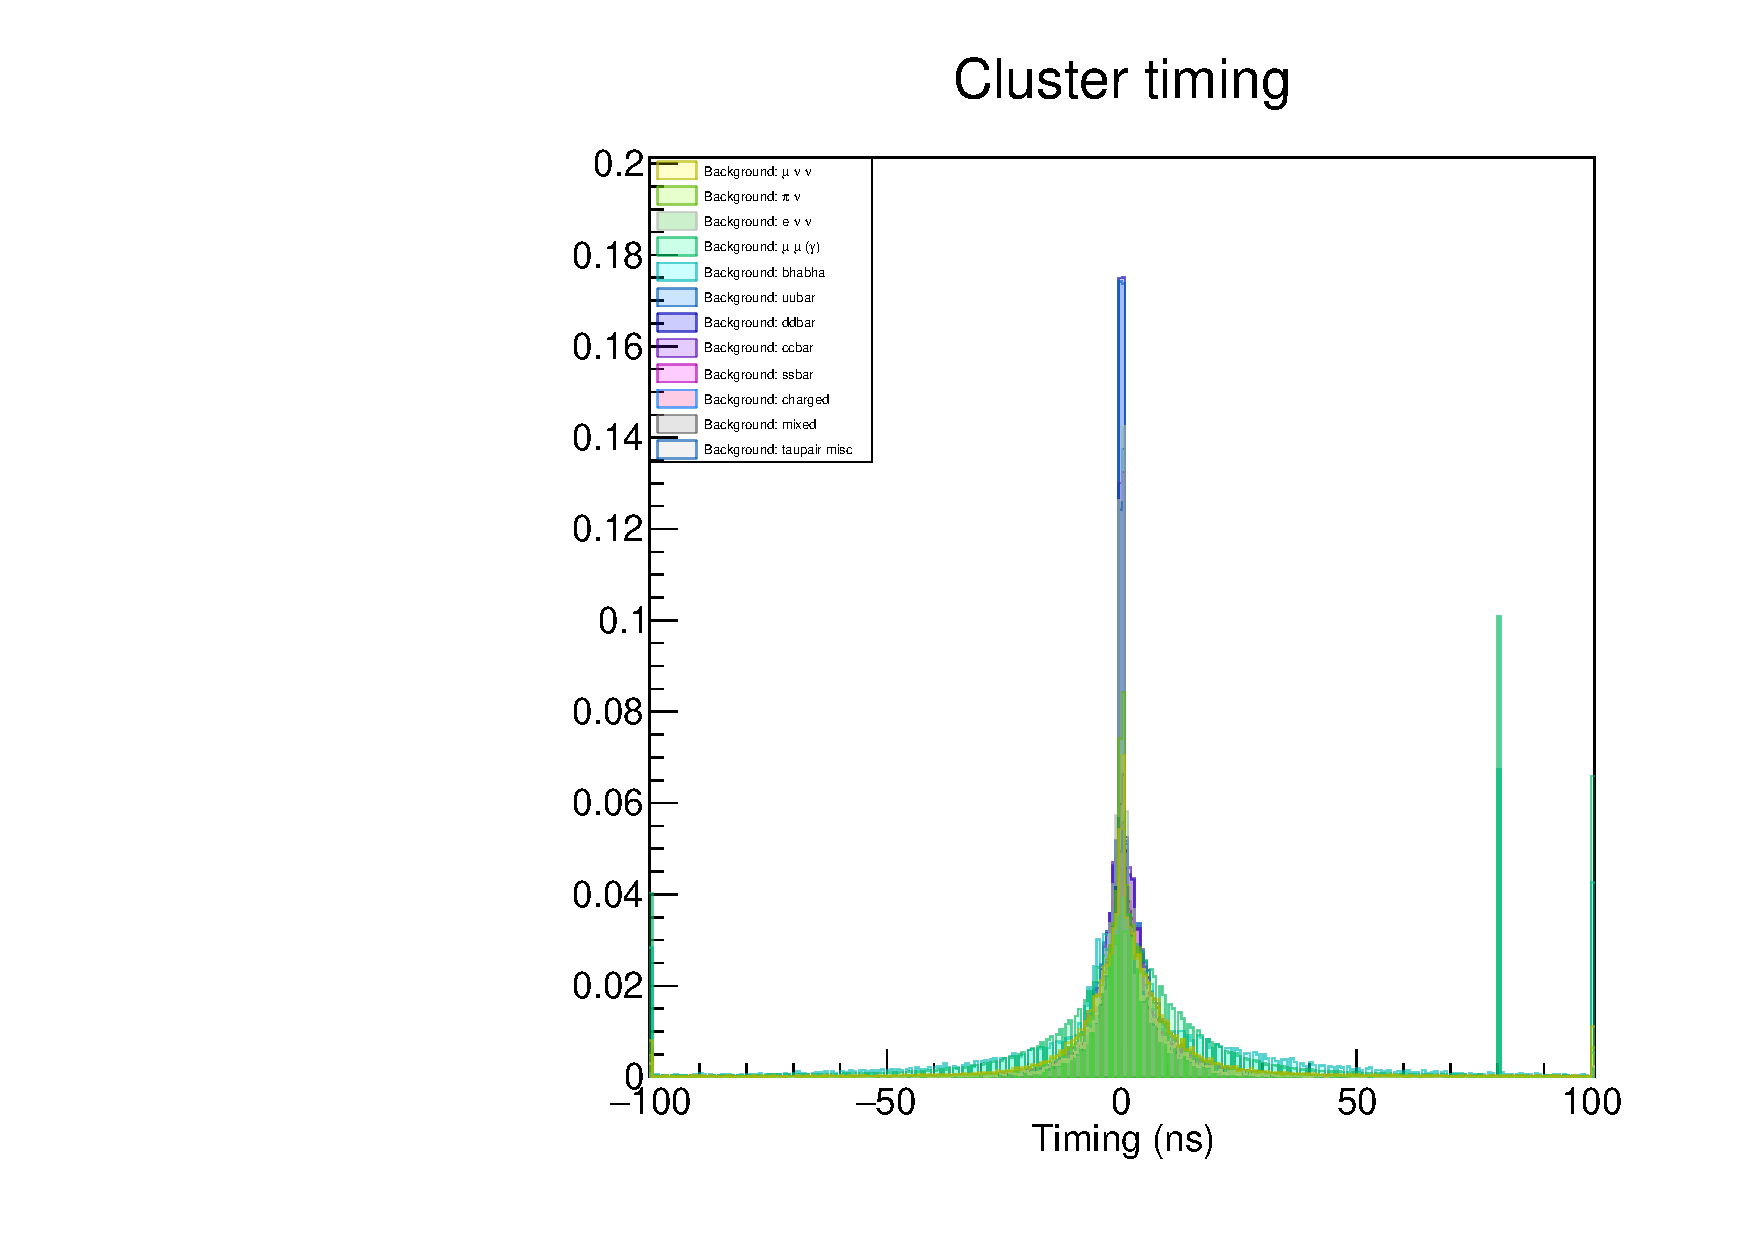
\includegraphics[width=\textwidth]{images/cluster-timing-new.pdf}
            \caption[]%
            {{\small}}    
            \label{fig:mean and std of net24}
        \end{subfigure}
        \caption{Comparisons of cluster timing with background MC (a) prior to ECL timing change and (b) after ECL timing change. Note the shift in peak by 80 units.}
    \end{figure}



\section{Implementation of beam backgrounds}

Signal and background MC was generated with simulated beam background. The most important sources have been generated by a dedicated accelerator group software within the Belle II collaboration. This software simulates particles travelling the detector and records the position and momentum of particles which leave the nominal beam trajectory and collide with the beam pipe or collimator (???). Detector response simulation is then processed for these particles to produce background samples of a given type. Separate backgrounds were made for electron (HER) and positron (LER) beams, due to differences in energies and currents. 

\begin{table}[h]
\centering
\begin{tabular}{lcr}
\hline
\multicolumn{1}{c}{type}      & source & \multicolumn{1}{c}{rate [MHz]} \\ \hline
radiative Bhabha              & HER    & \num{1320}                     \\
radiative Bhabha              & LER    & \num{1294}                     \\
radiative Bhabha (wide angle) & HER    & \num{40}                       \\
radiative Bhabha (wide angle) & LER    & \num{85}                       \\
Touschek scattering           & HER    & \num{31}                       \\
Touschek scattering           & LER    & \num{83}                       \\
beam-gas interactions         & HER    & \num{1}                        \\
beam-gas interactions         & LER    & \num{156}                      \\ \hline
\end{tabular}
\caption{Beam background types simulated at Belle II (REF - Belle II Simulation (Belle II note)). Rate is calculated}
\label{my-label}
\end{table}


Implemented background types are listed in Table XXXX.




For comparison, some samples of MC were generated without beam background. Comparisons between some measureables are shown in figures XXX, XXX, XXX below.

   \begin{figure}[h]
        \centering
        \begin{subfigure}[b]{0.475\textwidth}
            \centering
            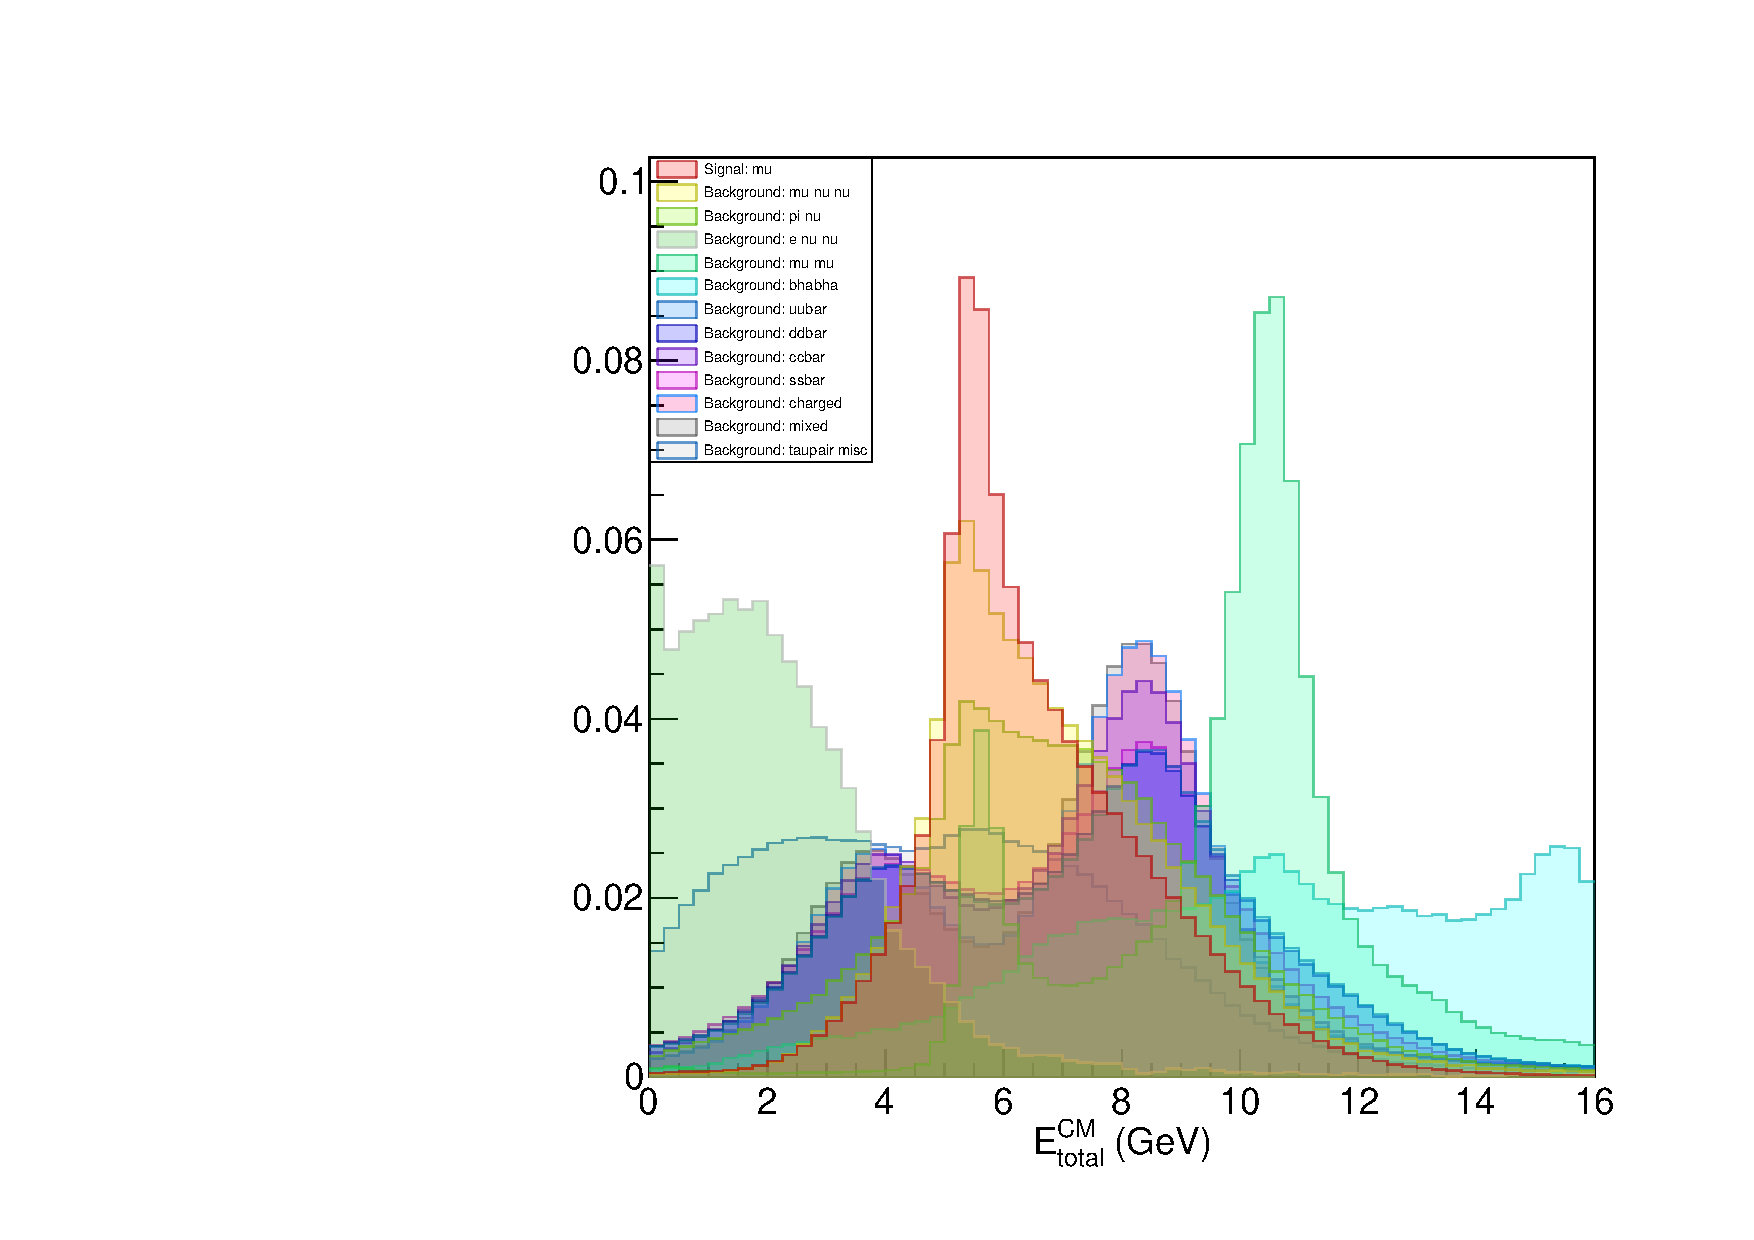
\includegraphics[width=\textwidth]{images/test.pdf}
            \caption[Network2]%
            {{\small Total center-of-mass energies w/o beam background}}    
            \label{fig:mean and std of net14}
        \end{subfigure}
        \hfill
        \begin{subfigure}[b]{0.475\textwidth}  
            \centering 
            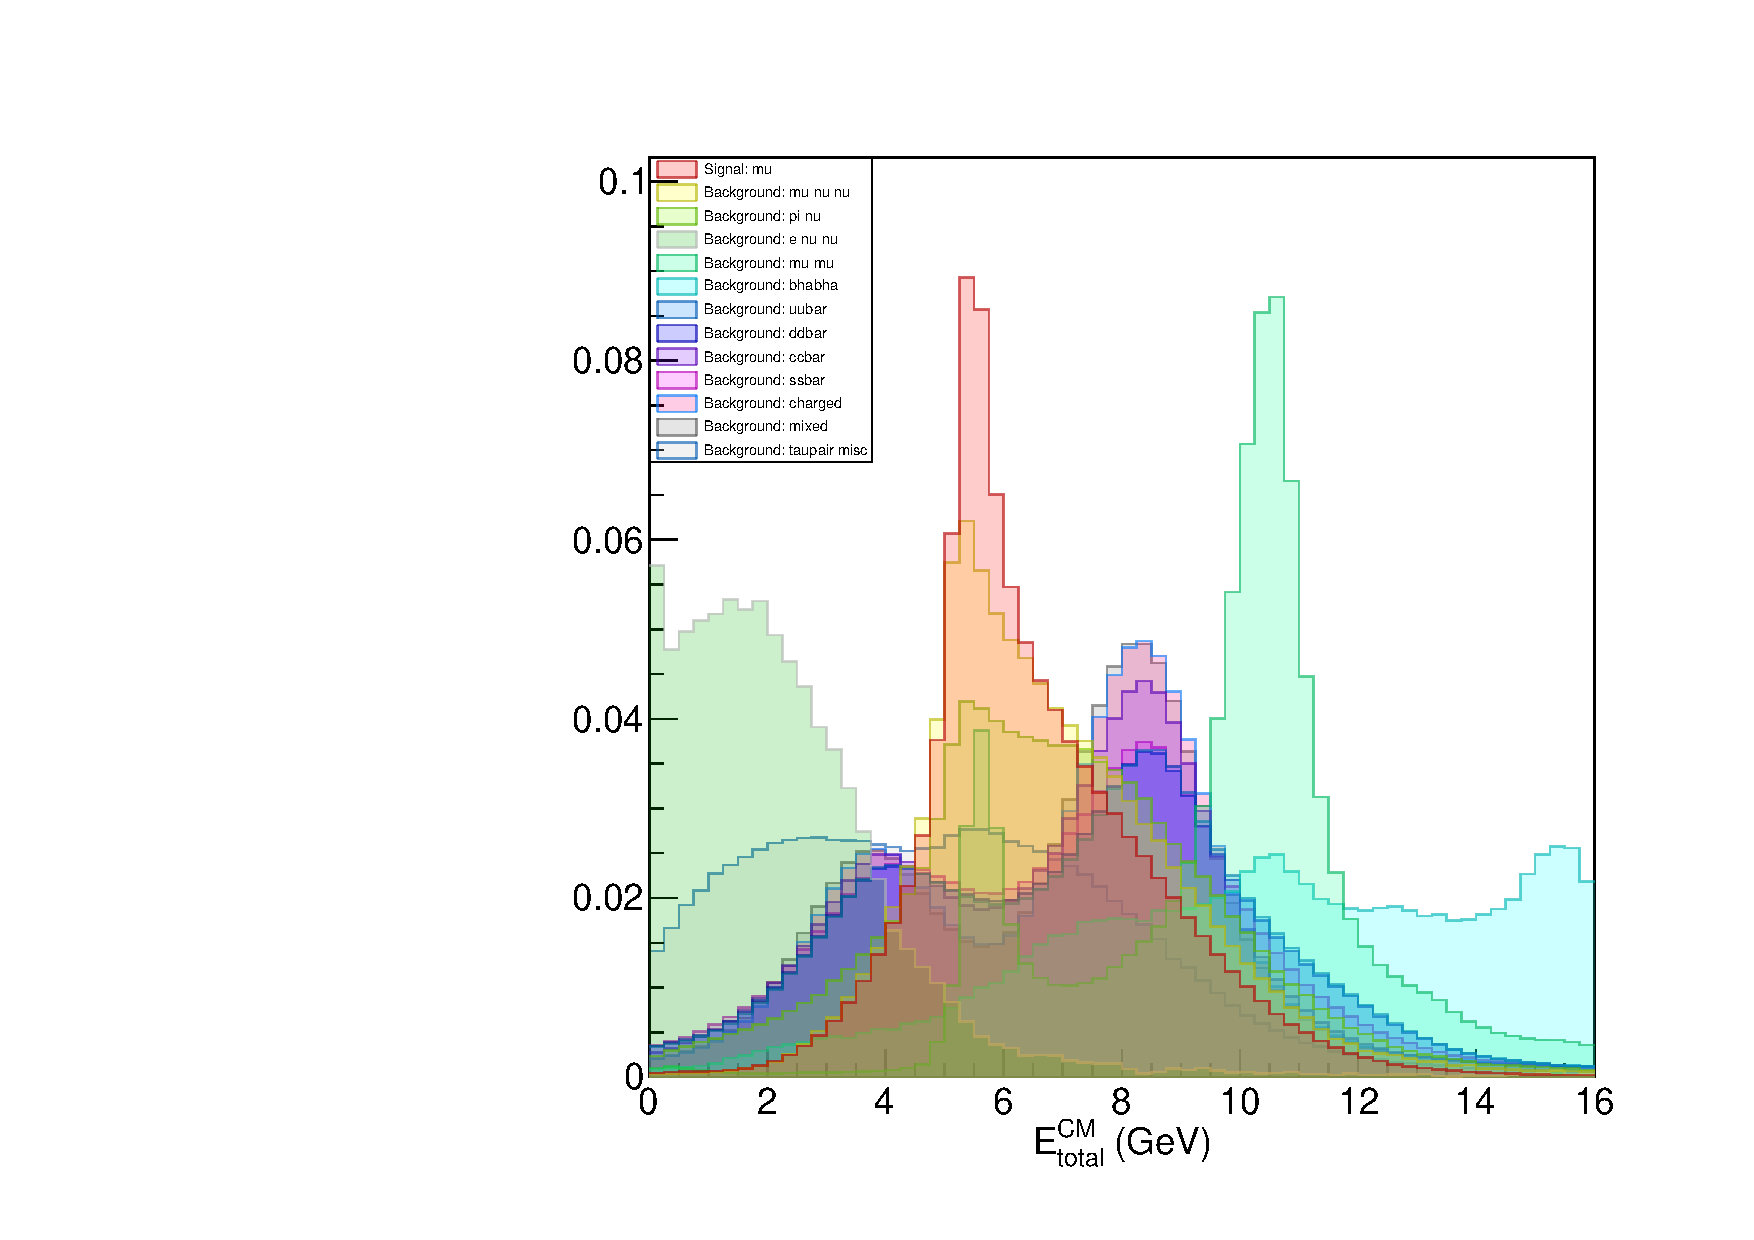
\includegraphics[width=\textwidth]{images/test.pdf}
            \caption[]%
            {{\small Total center-of-mass energies w/ beam background}}    
            \label{fig:mean and std of net24}
        \end{subfigure}
    \end{figure}
    
    
   \begin{figure}[h]
        \centering
        \begin{subfigure}[b]{0.475\textwidth}
            \centering
            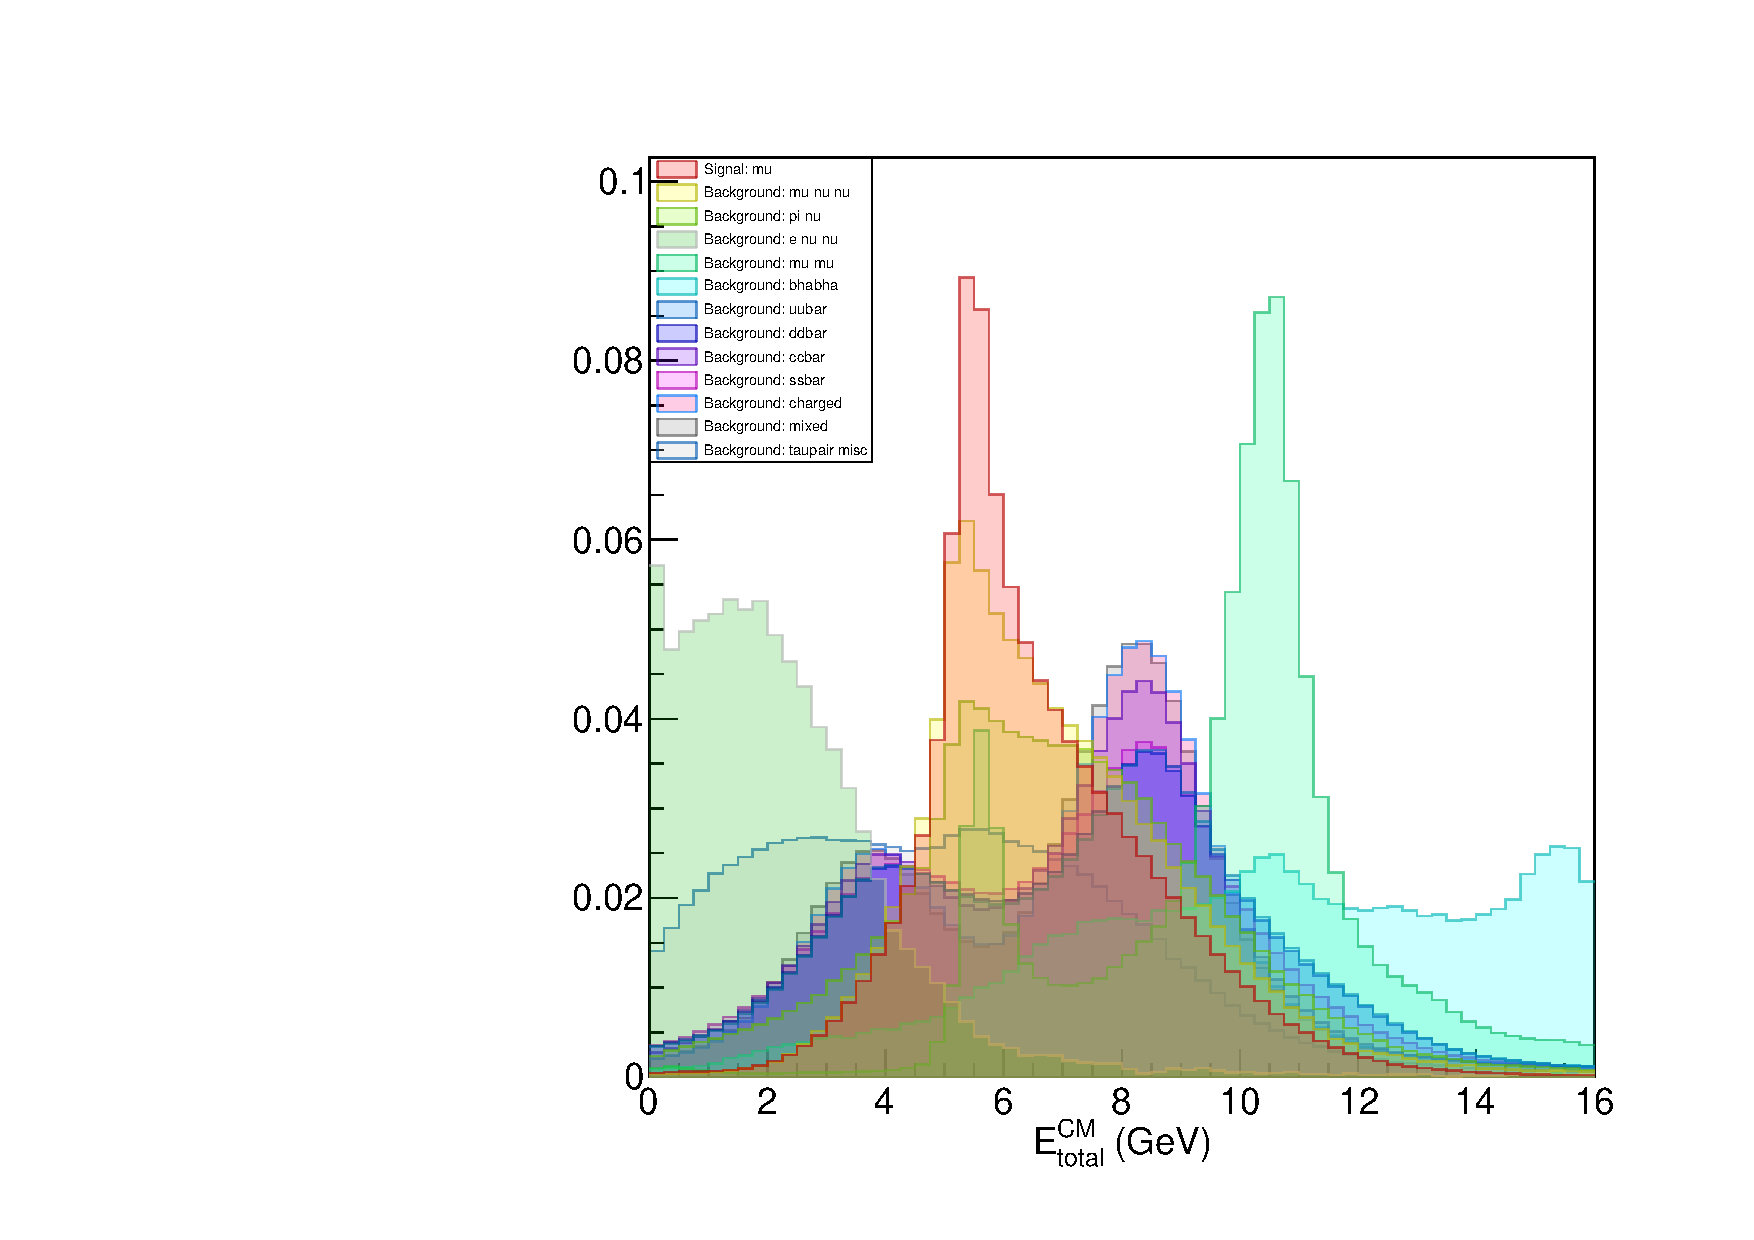
\includegraphics[width=\textwidth]{images/test.pdf}
            \caption[Network2]%
            {{\small Total center-of-mass energies w/o beam background}}    
            \label{fig:mean and std of net14}
        \end{subfigure}
        \hfill
        \begin{subfigure}[b]{0.475\textwidth}  
            \centering 
            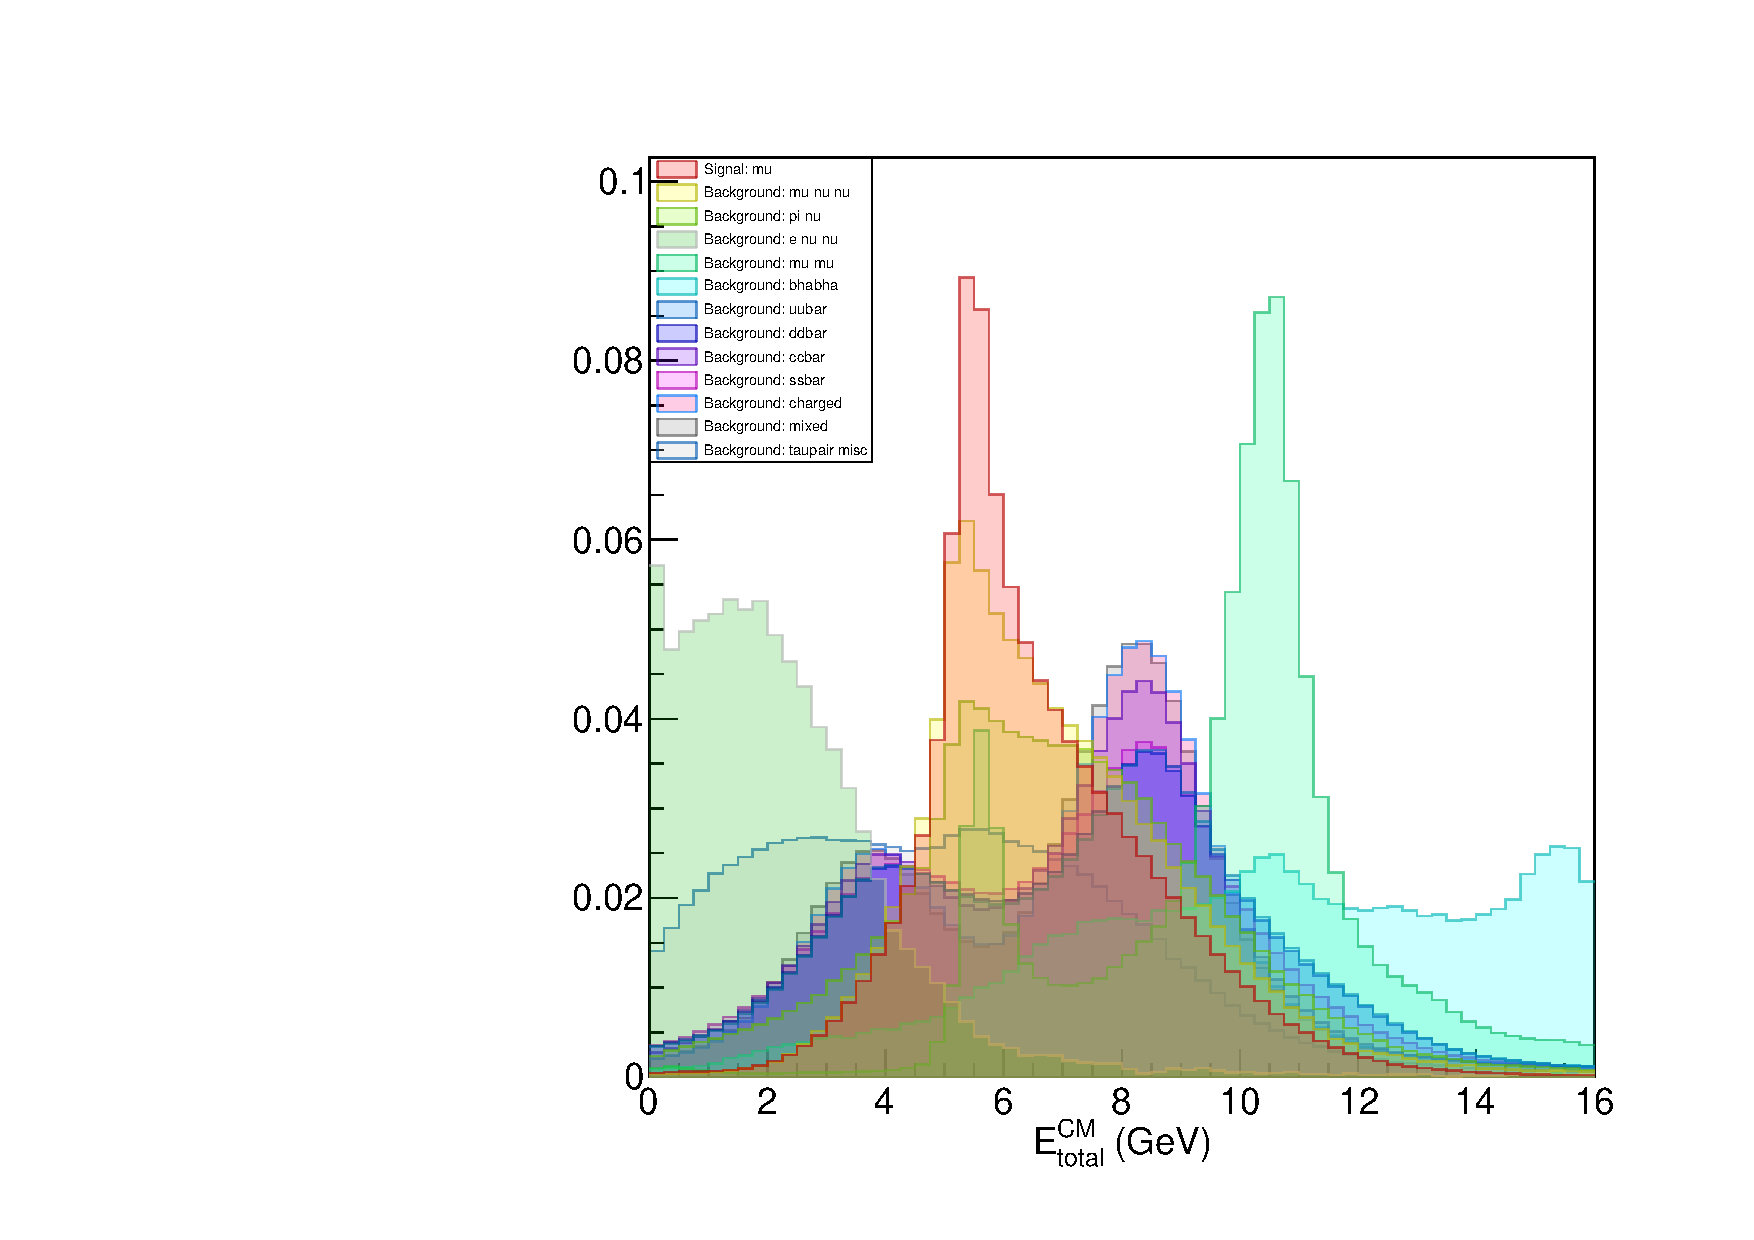
\includegraphics[width=\textwidth]{images/test.pdf}
            \caption[]%
            {{\small Total center-of-mass energies w/ beam background}}    
            \label{fig:mean and std of net24}
        \end{subfigure}
    \end{figure}
    
    
    
    
There are many differences between MC with and without beam background; only a few key points will be discussed here. Most obvious is the number of tracks recorded. Taking, for instance, our signal mode, we would expect for most events 2 or 4 tracks - one signal-side track corresponding to $\mu/e$, and one or three tracks on the tag-side (one- or three-pronged) coming from standard model $\tau$ decays, which are dominantly one- or three-pronged. Beam background particles in the detector produce a number of new tracks (as well as clusters) which are tracked by sub-detector components, then later reconstructed.

Kinematic variables such as energy and momentum are also obviously affected by beam background. We observe an increase in low energy and low momentum tracks; in these cases low energy beam background particles have been misidentified as signal- or tag-side particles originating from tau-pair processes.





\pagebreak
%------------------------------------------------------------------

\chapter{Reconstruction}

Reconstruction of events was performed through \texttt{basf2}. The generated MC consists of information about charged tracks travelling through the detector geometry and interacting with sub-detectors, as well as cluster information relating 
to photons from the ECL, among other information. 


\section{Process}

\textbf{Belle II Note: Belle II Reconstruction Software and Performance}

To reconstruct events, we fill lists of particles by categorising tracks as specific charged particles - muons, electrons or pions, and by associating clusters with photons. These categorisations are performed with loose criteria to remove obvious background events. Tracks with PID values greater than 0.1 (or 0.5?) are considered muons, and similar for electrons and pions; the photon list is populated by clusters passing a ``goodness'' test. 



DISCUSS SIGNAL SIDE/TAG SIDE (+signal track, signal photon).


In the following, the \emph{signal track} describes the reconstructed track associated with the final state electron or muon from $\tau\to\ell\gamma$; similarly the \emph{signal photon} describes the cluster associated with the final state photon. These terms do not necessarily refer to the physical charged track or photon from the signal modes under analysis - 

The signal-side particles do not necessarily refer to the physical charged particle or photon coming from the signal modes under analysis; misidentified particles (such as a pion being identified as a muon during reconstruction) or particles from different decay processes (such as a muon from the tau process $\tau\to\mu\nu\nu$).


We reconstruct the signal side tau as $\tau \to \mu \gamma$ for the muon mode, or $\tau \to e \gamma$ for the electron mode. The tag side tau is reconstructed by requiring at least one muon, electron or charged pion. In addition to PID cuts, we also apply loose cuts to our $\Delta E$ and $M_{\text{inv}}$. We define our signal region variables as
\begin{align}
\Delta E &= E^{\text{CM}}_{\text{signal }\tau} - E_{\text{beam}}/2,\\
M_{\text{inv}} &= \text{invariant mass of reconstructed signal side tau},
\end{align}
where $E^{\text{CM}}_{\text{signal }\tau}$ is the center-of-mass energy of the reconstructed signal-side tau, and $E_{\text{beam}}$ is the total center-of-mass energy of the electron-positron beam system. Nominally we expect signal events to have $\Delta E\sim 0$ and $M_{\text{inv}}\sim m_{\tau}$; signal region selection is further discussed in Section XXXX.

Once background has been sufficiently reduced through use of selection criteria, signal candidates will be chosen from events in the $\Delta E$ vs. $M_{\text{inv}}$ phase space. As such we cut (???) only very loosely on these criteria wherever possible; in reconstruction we require $\SI{-0.4}{GeV} < \Delta E < \SI{0.2}{GeV}$ and $\SI{1.6}{GeV} < M_{\text{inv}} < \SI{1.9}{GeV}$ for the signal side tau. 

The number of events over which reconstruction was performed, as well as the percentage of events after reconstruction/events before reconstruction (which we shall call \emph{reconstruction efficiency} $\epsilon_{\text{recon}}$), is shown in TABLE XXXX below (I WANT TO REWORD THIS).


\section{Reconstruction efficiencies}

\begin{table}[h]
\centering
\begin{tabular}{lrrr}
\textbf{Event type}         & \textbf{events in} & \textbf{events out} & $\mathbf{\epsilon_{\text{recon}}}$ \\ \hline 
\rowcolor[HTML]{EFEFEF} 
$\tau\to\mu\gamma$       & \num{3200000}        & \num{5435660}      & $\SI{169.86}{\percent}$                   \\
\rowcolor[HTML]{EFEFEF} 
$\tau\to e \gamma$      & \num{2550000}       & \num{4155023}       & $\SI{162.94}{\percent}$                            \\
$\tau\to\mu\nu\nu$      & \num{127998320}         & \num{542504}          & $\SI{0.42}{\percent}$           \\
$\tau\to\pi\nu$         & \num{267245200}       & \num{861406}          & $\SI{0.32}{\percent}$            \\
$\tau\to e\nu\nu$       & \num{131086160}        & \num{87848}         & $\SI{0.07}{\percent}$      \\
$\tau\to\text{generic}$  & \num{208870320}       & \num{1843380}          & $\SI{0.88}{\percent}$         \\
$e^+ e^- \to \mu^+ \mu^- (\gamma)$   & \num{148600000}    & \num{5159295}     & $\SI{3.47}{\percent}$   \\
$e^+ e^- \to e^+ e^- (\gamma)$      & \num{15630000}      & \num{370496}       & $\SI{2.37}{\percent}$     \\
$e^+ e^- \to u \bar{u}$       & \num{1268991935}           & \num{52373200}  & $\SI{4.13}{\percent}$ \\
$e^+ e^- \to d \bar{d}$        & \num{317048262}       & \num{12987072}      & $\SI{4.10}{\percent}$       \\
$e^+ e^- \to c \bar{c}$        & \num{1039855756}       & \num{48007101}           & $\SI{4.62}{\percent}$          \\
$e^+ e^- \to s \bar{s}$       & \num{289900586}     & \num{11122646}            & $\SI{3.84}{\percent}$         \\
$e^+ e^- \to B^+ B^-$     & \num{451320000}       & \num{46498047}           & $\SI{10.30}{\percent}$          \\
$e^+ e^- \to B^0 \bar{B}^0$       & \num{427680000}           & \num{46912228}        & $\SI{10.97}{\percent}$              
\end{tabular}
\caption{Reconstruction efficiency (un-scaled events)}
\label{my-label}
\end{table}

\section{Fake rates}


\pagebreak


\chapter{Event signatures}

We discuss expected energies, kinematics and signal-side event topologies with comparison to MC data. Knowledge of event topologies is important in selecting regions in phase space to remove when optimising the ratio of signal-to-background. 

\section{Signal}

This also serves also validation of the signal MC - since it was generated and used by an individual rather than by multiple people within the Belle II Collaboration, the possibility of errors in generation and reconstruction are higher than for background MC. 


\subsection{Muon mode}

The mode $\tau\to\mu\gamma$ has a simple signal side, with only one track and one photon, and no missing energy (in the form of neutrinos). If we assume that on average both $\tau$ particles generated in the $e^+ e^-$ collision share equally the energy generated in the interaction, we expect the mean signal-side center-of-mass frame energy to be $\SI{5.5}{GeV}$. No physical preference is given to the energy distribution between the signal muon and signal photon, so their center-of-mass energies should be normally distributed around $\SI{2.75}{GeV}$. Recalling the relation between energy, momentum and mass,

\begin{equation}
E^2 = p^2 + m^2,
\end{equation}
since the muon energy is much greater than its mass of $\SI{105.66}{MeV/c^2}$ this can simplify to
\begin{equation}
E^2 \approx p^2.
\end{equation}

Note that $p$ is the magnitude of the particle's 3-momentum.

We can predict and compare with MC several topological measureables, such as polar angle (i.e. angle from an axis parallel to the beam trajectory) as well as opening angles between particles; this is done for several key measureables. The average opening angle between the signal muon and signal photon in the center-of-mass frame can be calculated by boosting the expected back-to-back pair from the signal $tau$ frame into the lab frame.

CALCULATIONS.

Similarly for SOME OTHER PAIRING,

CALCULATIONS.

As shown in figures XXXX below, the MC matches the predicted kinematics and topologies for the muon mode.


\begin{figure}[h]
\centering
\begin{minipage}{.5\textwidth}
  \centering
  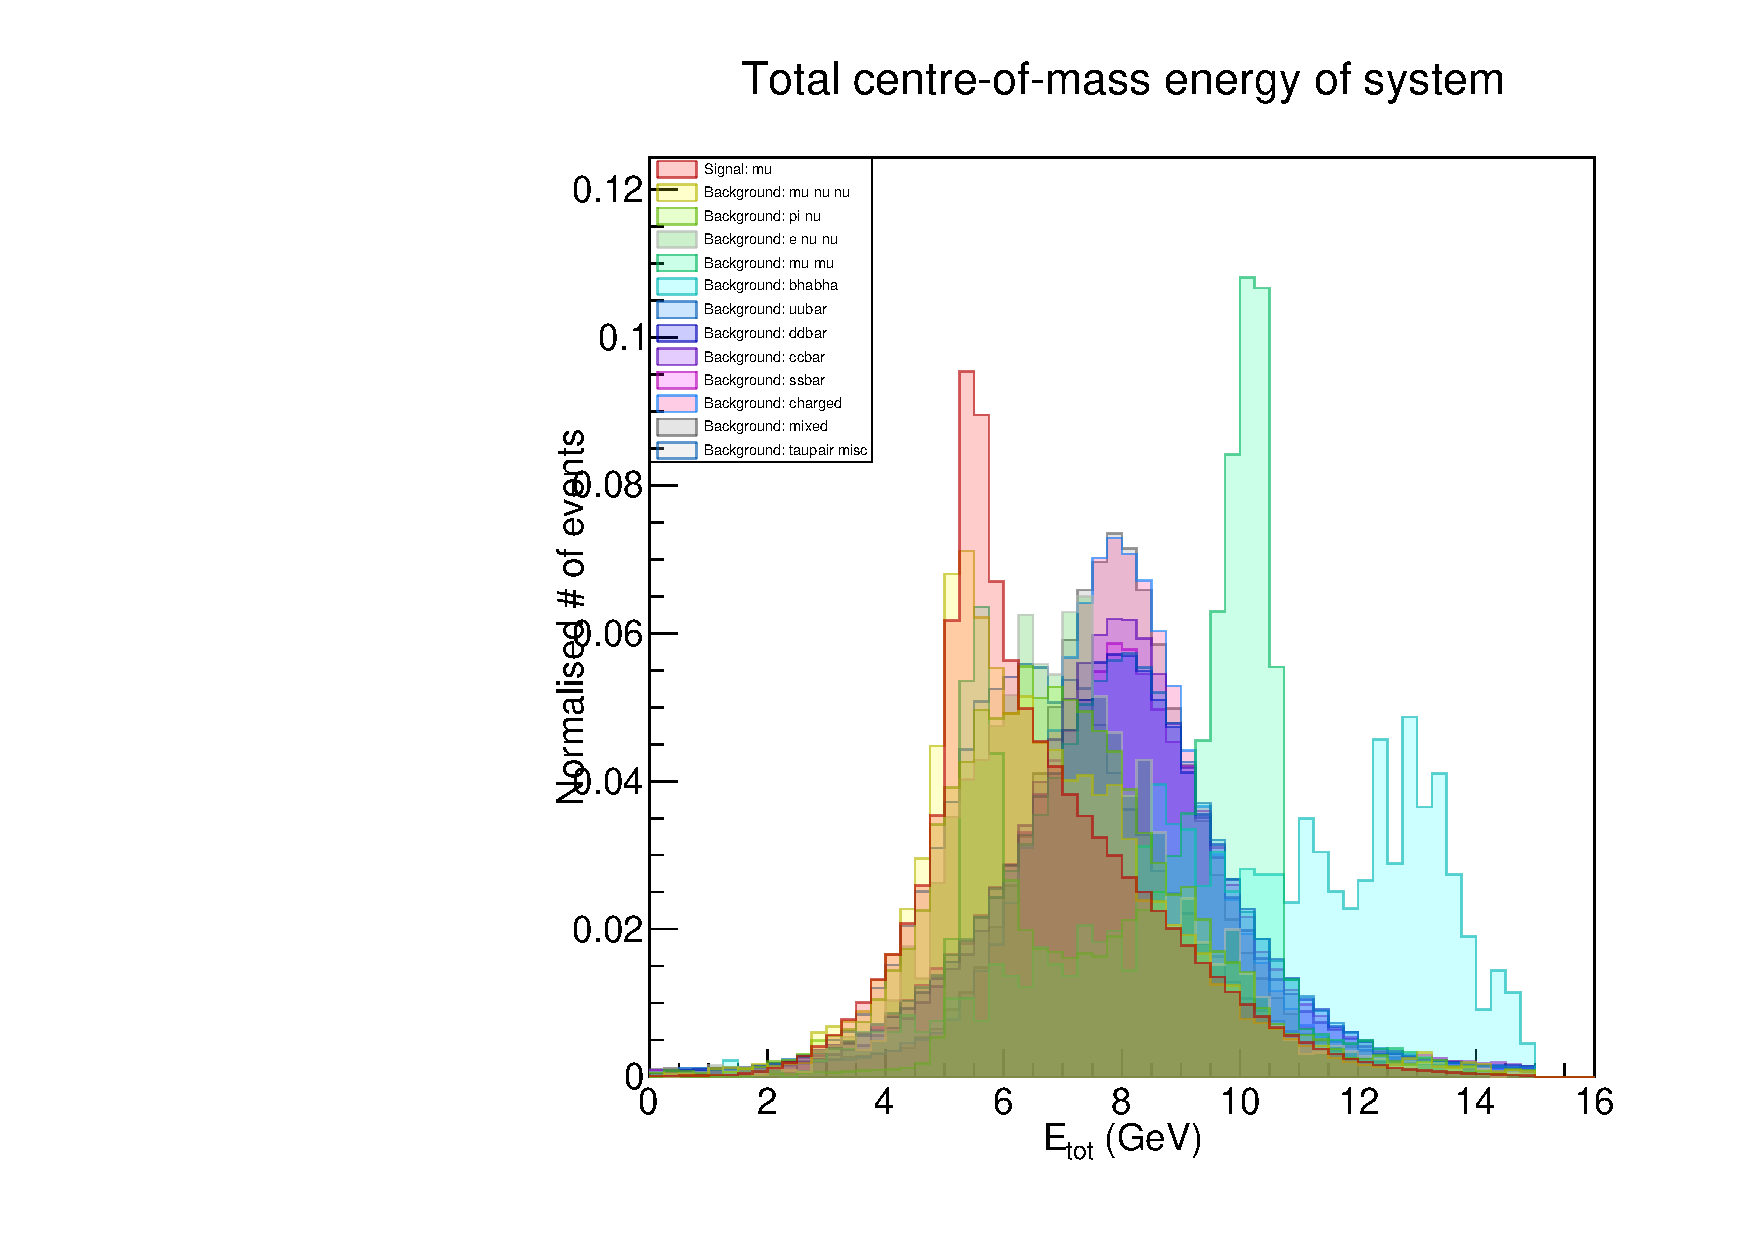
\includegraphics[width=\linewidth]{images/stack/stack_cut6_totalCM_E.pdf}
  \captionof{figure}{A figure}
  \label{fig:test1}
\end{minipage}%
\begin{minipage}{.5\textwidth}
  \centering
  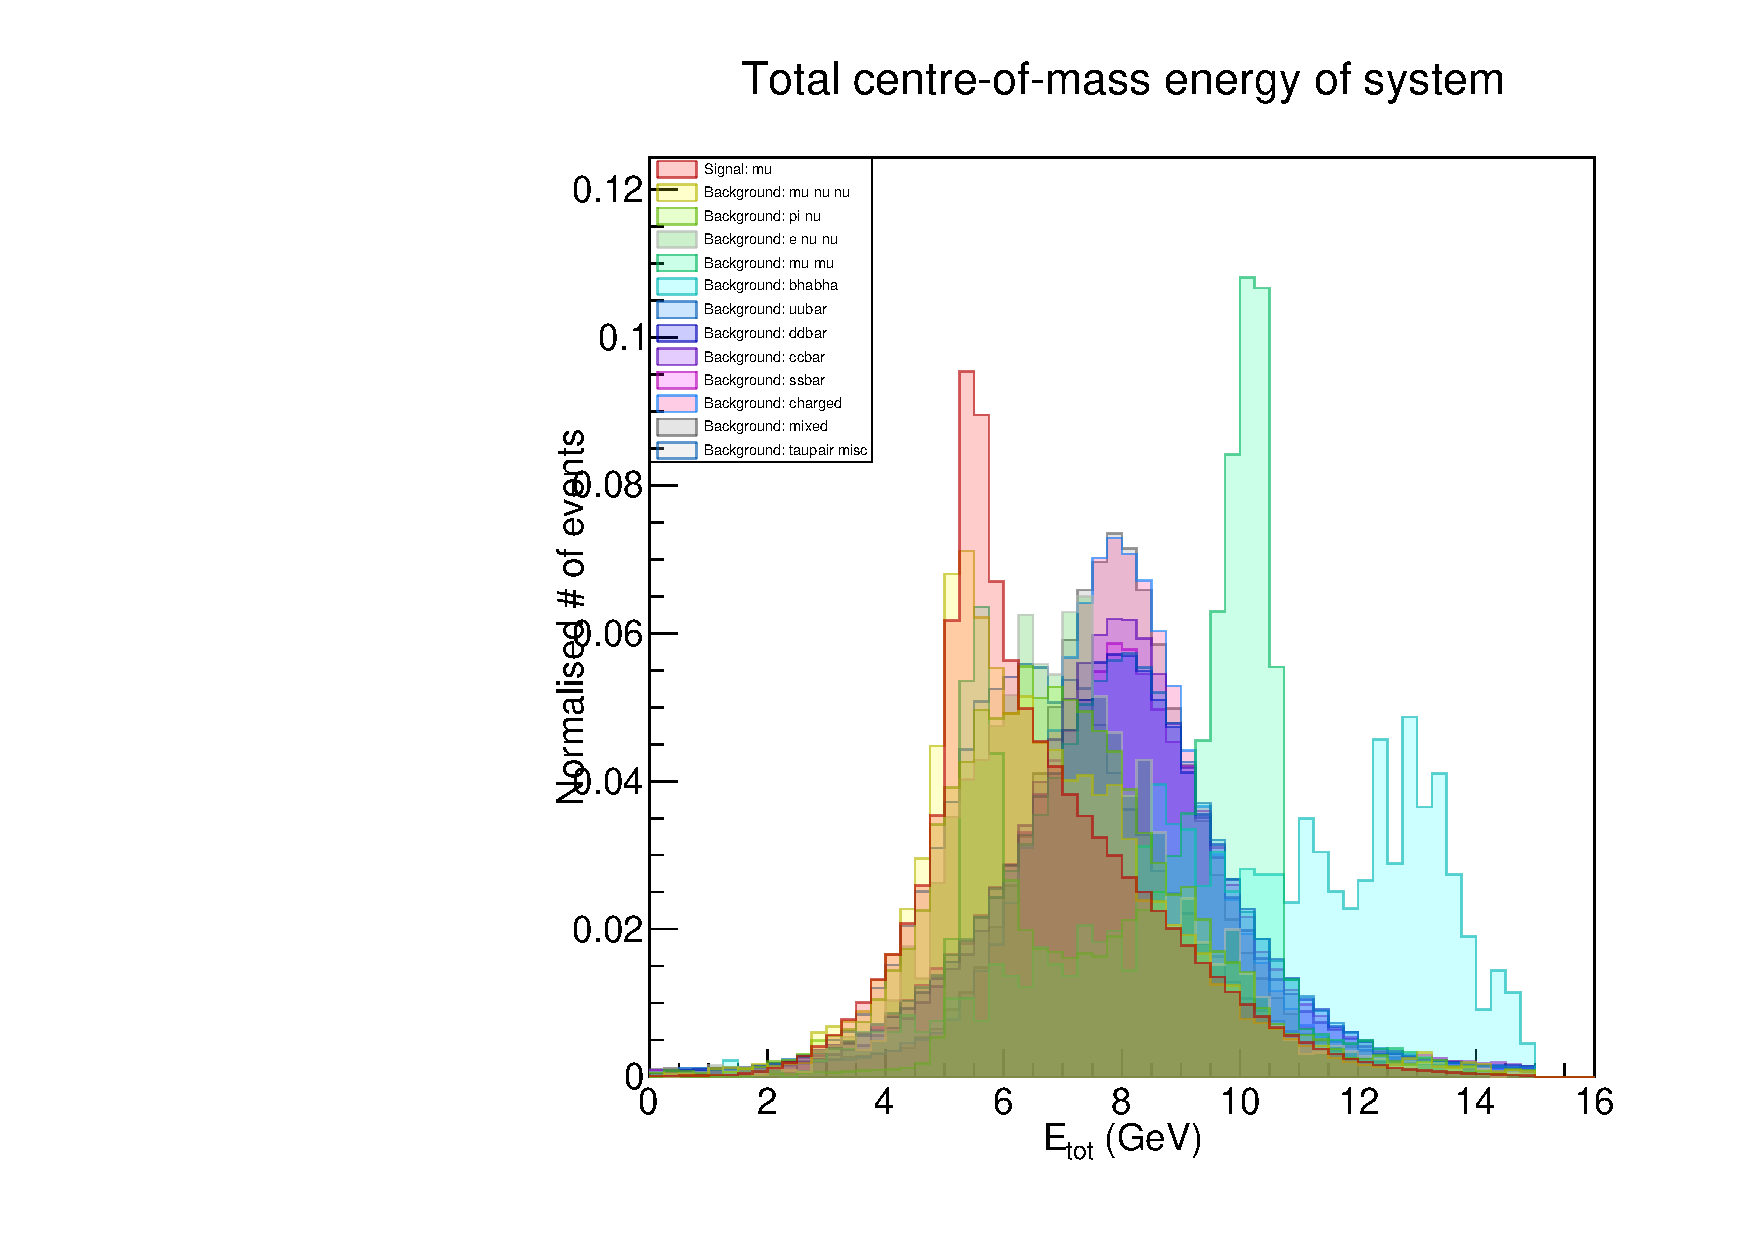
\includegraphics[width=\linewidth]{images/stack/stack_cut6_totalCM_E.pdf}
  \captionof{figure}{Another figure}
  \label{fig:test2}
\end{minipage}
\end{figure}

\begin{figure}[h]
\centering
\begin{minipage}{.5\textwidth}
  \centering
  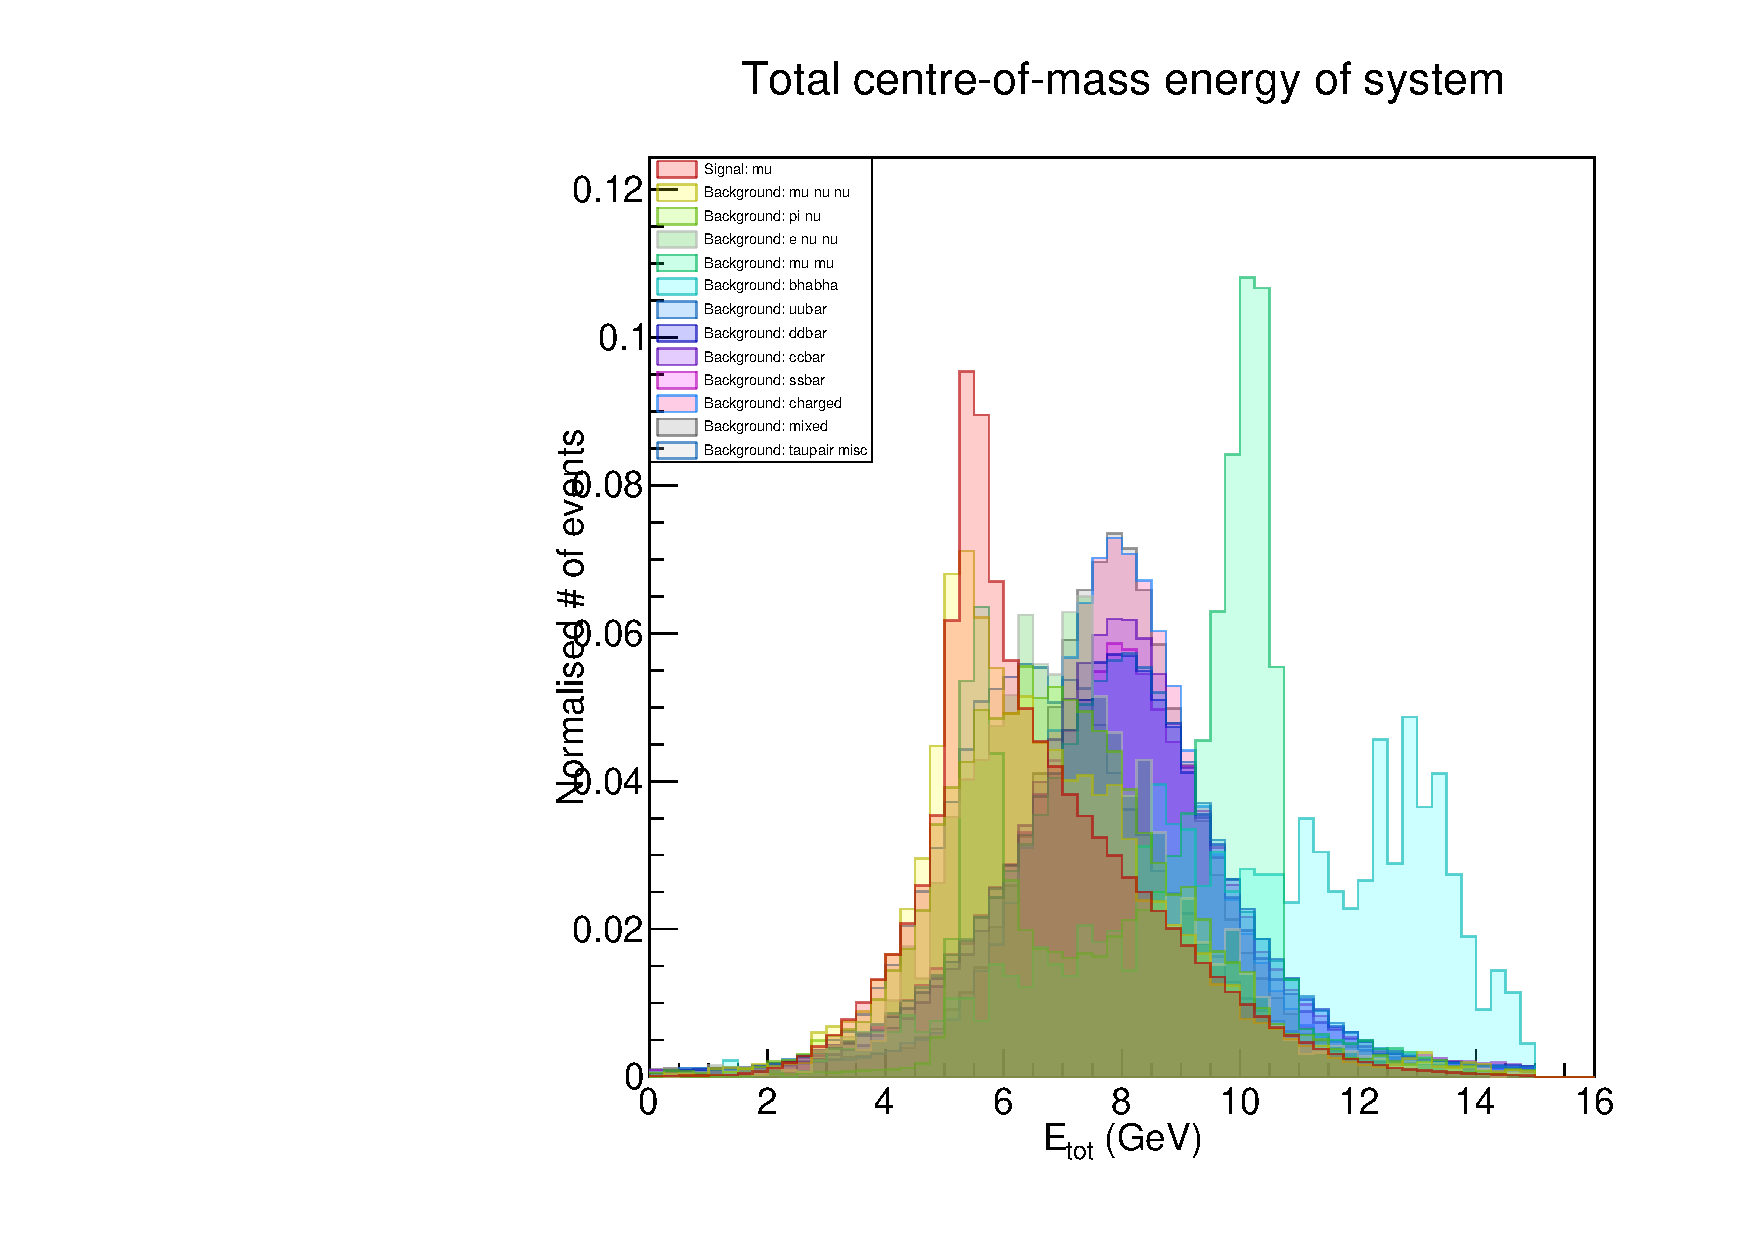
\includegraphics[width=\linewidth]{images/stack/stack_cut6_totalCM_E.pdf}
  \captionof{figure}{A figure}
  \label{fig:test1}
\end{minipage}%
\begin{minipage}{.5\textwidth}
  \centering
  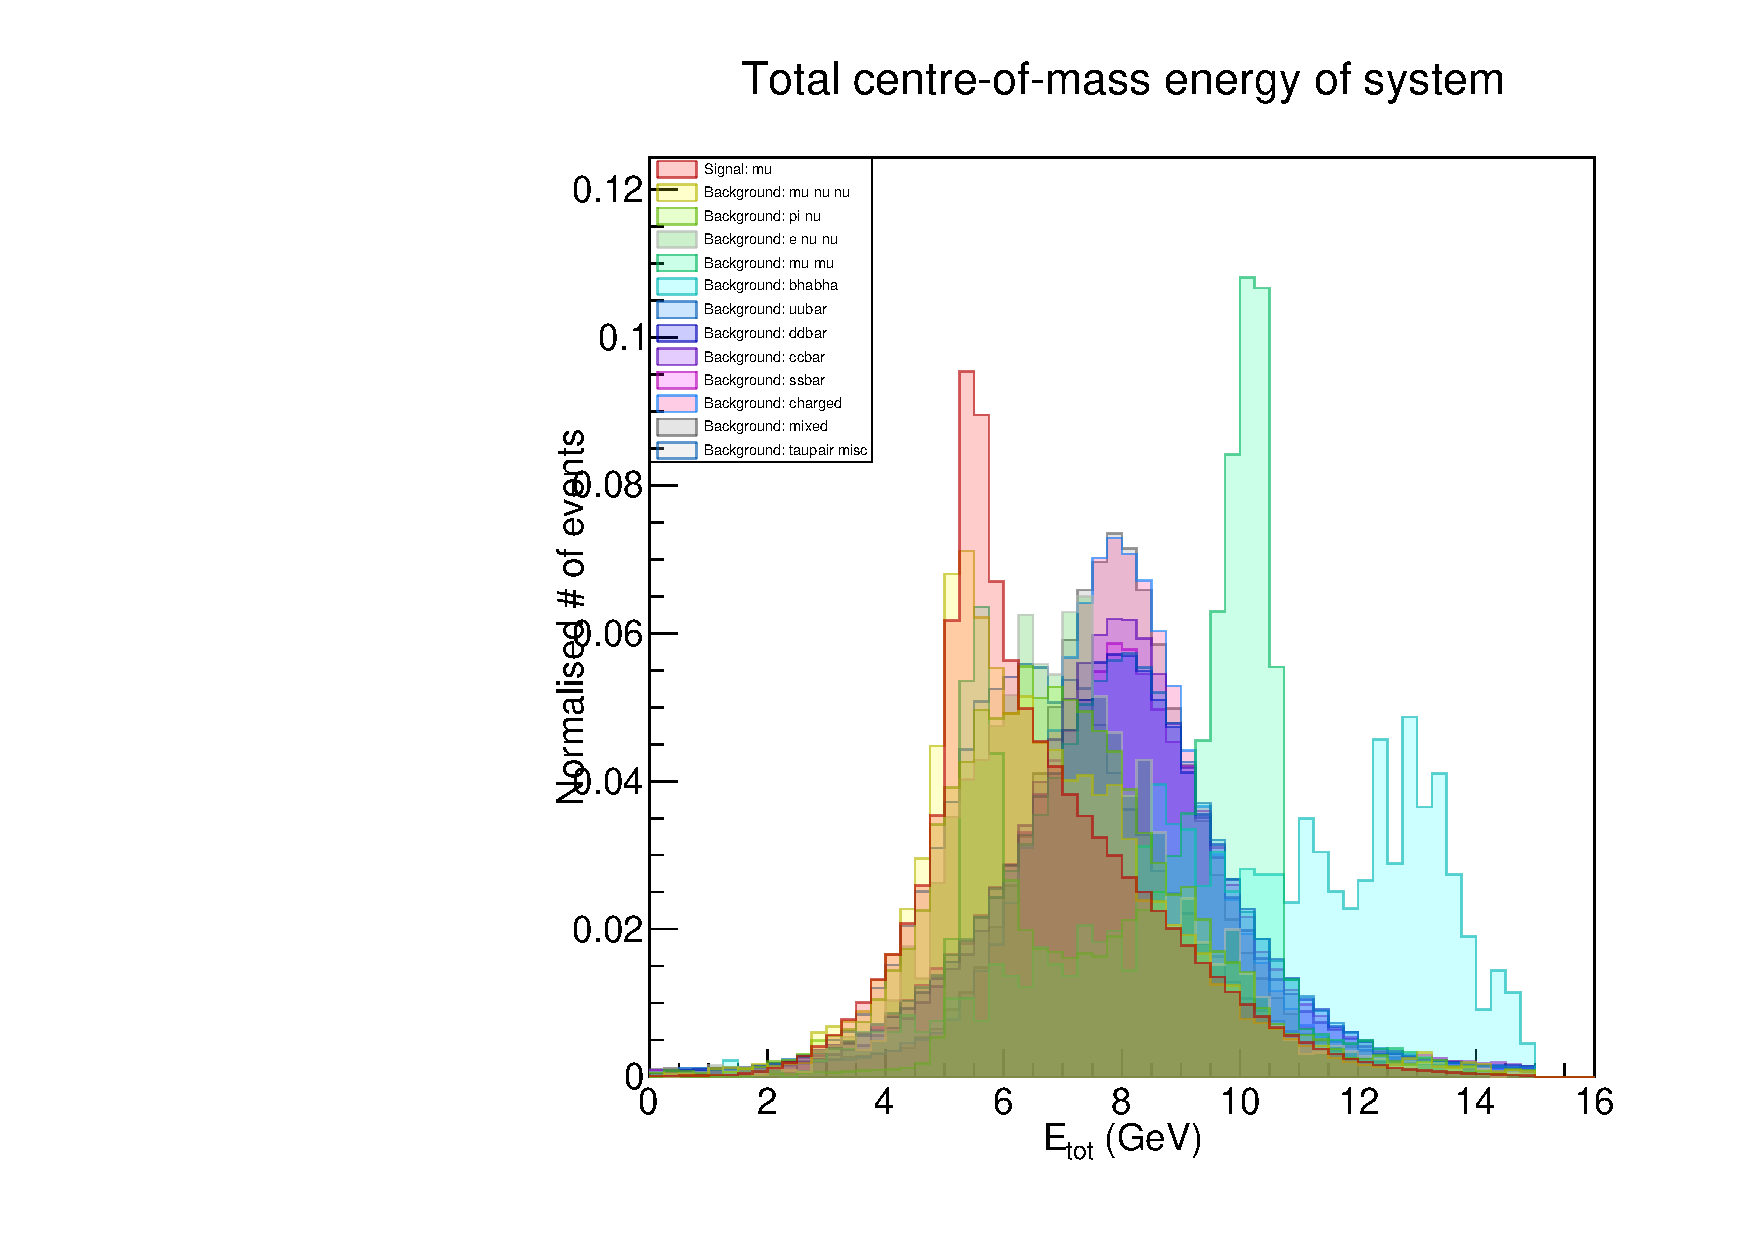
\includegraphics[width=\linewidth]{images/stack/stack_cut6_totalCM_E.pdf}
  \captionof{figure}{Another figure}
  \label{fig:test2}
\end{minipage}
\end{figure}

\subsection{Electron mode}

Much of the kinematics and topologies as described for the signal muon mode also applies to the signal electron mode. However, it is prudent to note the major difference between the two final state charged particles - specifically the difference in mass. Muons have mass $\SI{105.66}{MeV/c^2}$, over 200 times heavier than electrons, with mass of $\SI{0.511}{MeV/c^2}$. Due to their lighter mass, electrons lose far more energy due to bremsstrahlung (braking radiation), as given by

\begin{align}
P &= \text{radiated power} = \frac{e^2a^2 \gamma^4}{6},
\intertext{where}
e &= \text{electron charge},\\
a&= \text{particle acceleration},\\
\lambda &= \text{relativistic factor},\\
\end{align}
and we have of course taken particle physics units $c=\pi=\epsilon_0 = 1$. Since $E=\gamma mc^2$, radiated power from bremsstrahlung goes as $m^{-4}$; electrons lose more energy via bremsstrahlung than muons by factor $\left(m_{\mu}/m_{e}\right)^{4} \sim 200^4$.

This energy in the form of photons is deposited in the ECL clusters; a non-negligible amount of radiation from beam background is also deposited in these clusters, making accurate energy reconstruction of the signal electron difficult (??? is this right, or is it just that the electron has less energy? What is the ``energy/momentum'' variable.... E/P at creation?). Due to this energy loss we see a different energy and momentum 	signature for the signal track compared to the muon mode; peaks for both are located around XXXX GeV, but a large fraction of events have energies much lower.

Accurate reconstruction via \texttt{basf2} is more difficult for these lighter particles, with only a fraction of $\tau\to e\gamma$ events having a reconstructed $\tau$ invariant mass peak anywhere near the $\tau$ mass.


\begin{figure}[h]
\centering
\begin{minipage}{.5\textwidth}
  \centering
  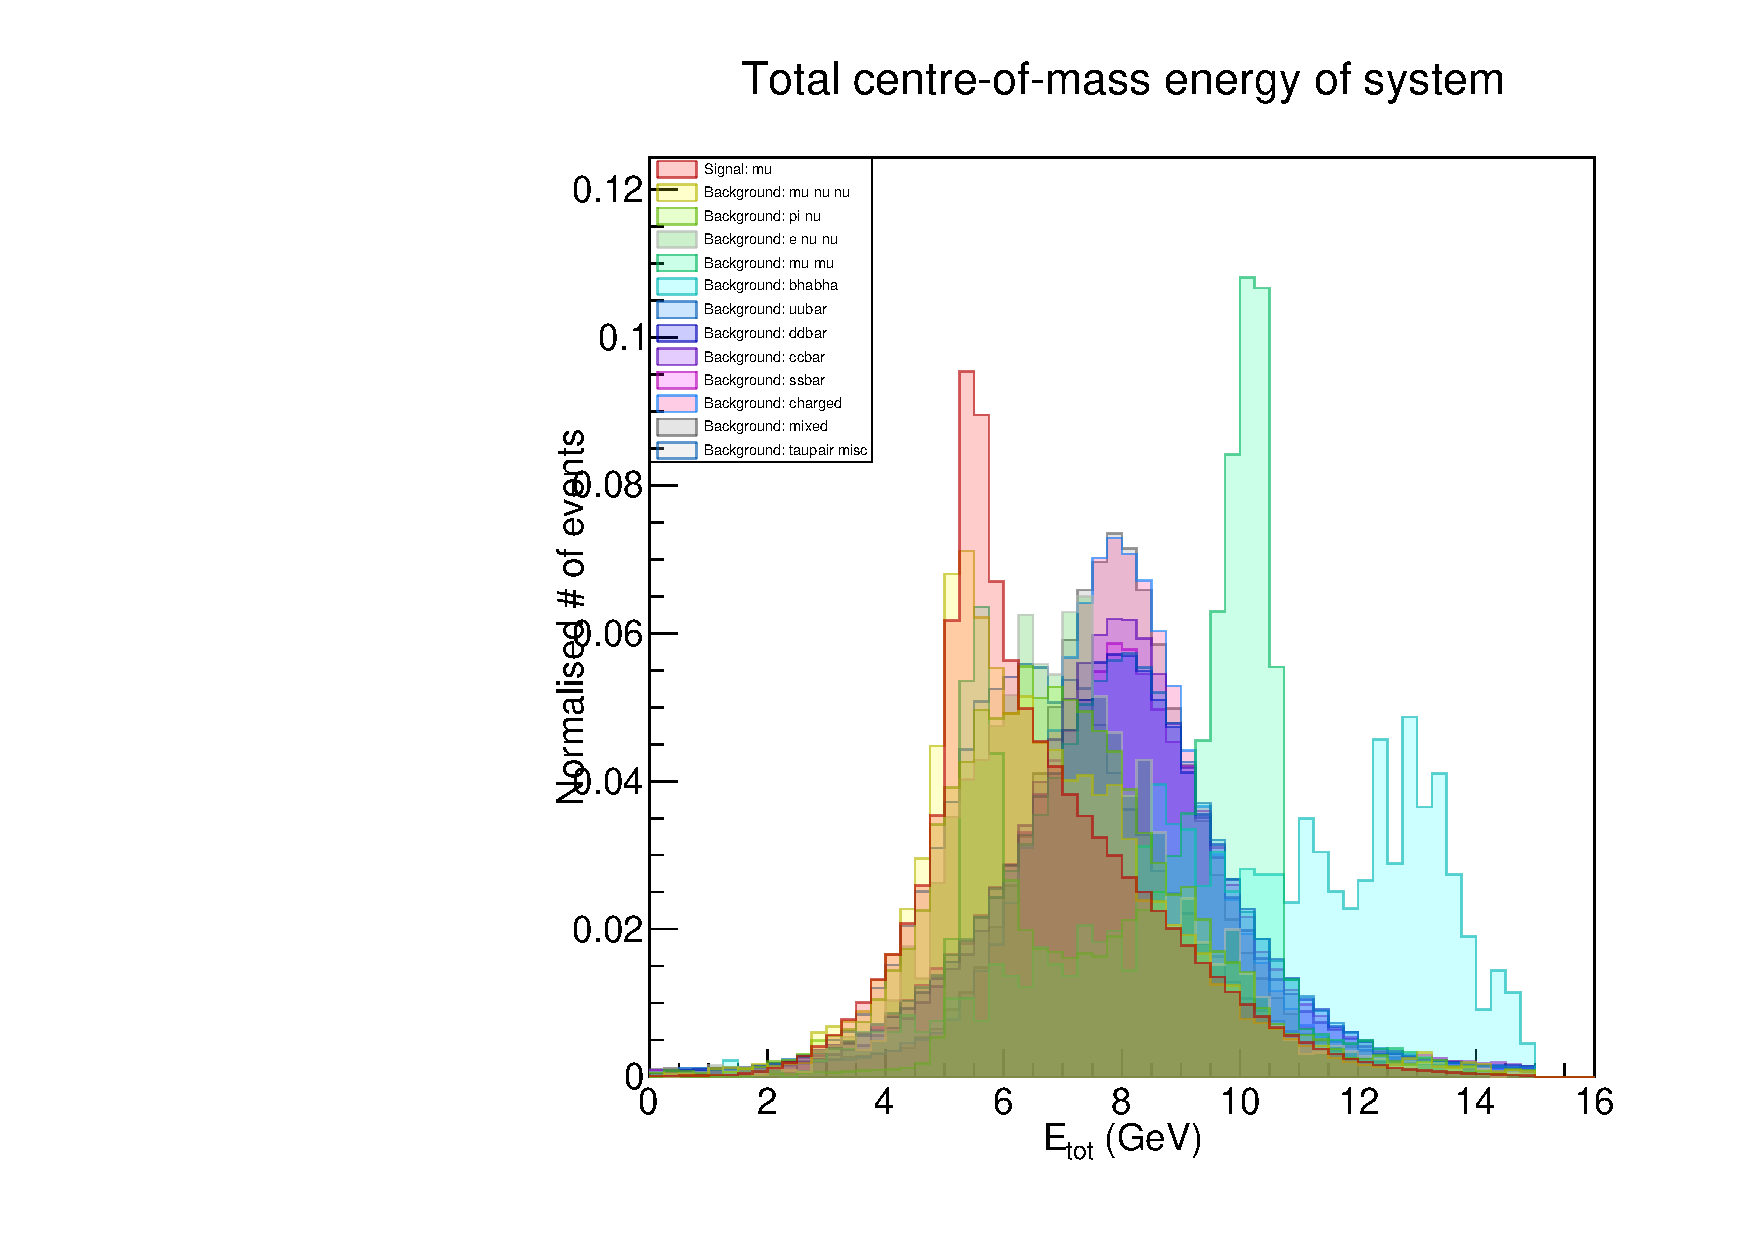
\includegraphics[width=\linewidth]{images/stack/stack_cut6_totalCM_E.pdf}
  \captionof{figure}{A figure}
  \label{fig:test1}
\end{minipage}%
\begin{minipage}{.5\textwidth}
  \centering
  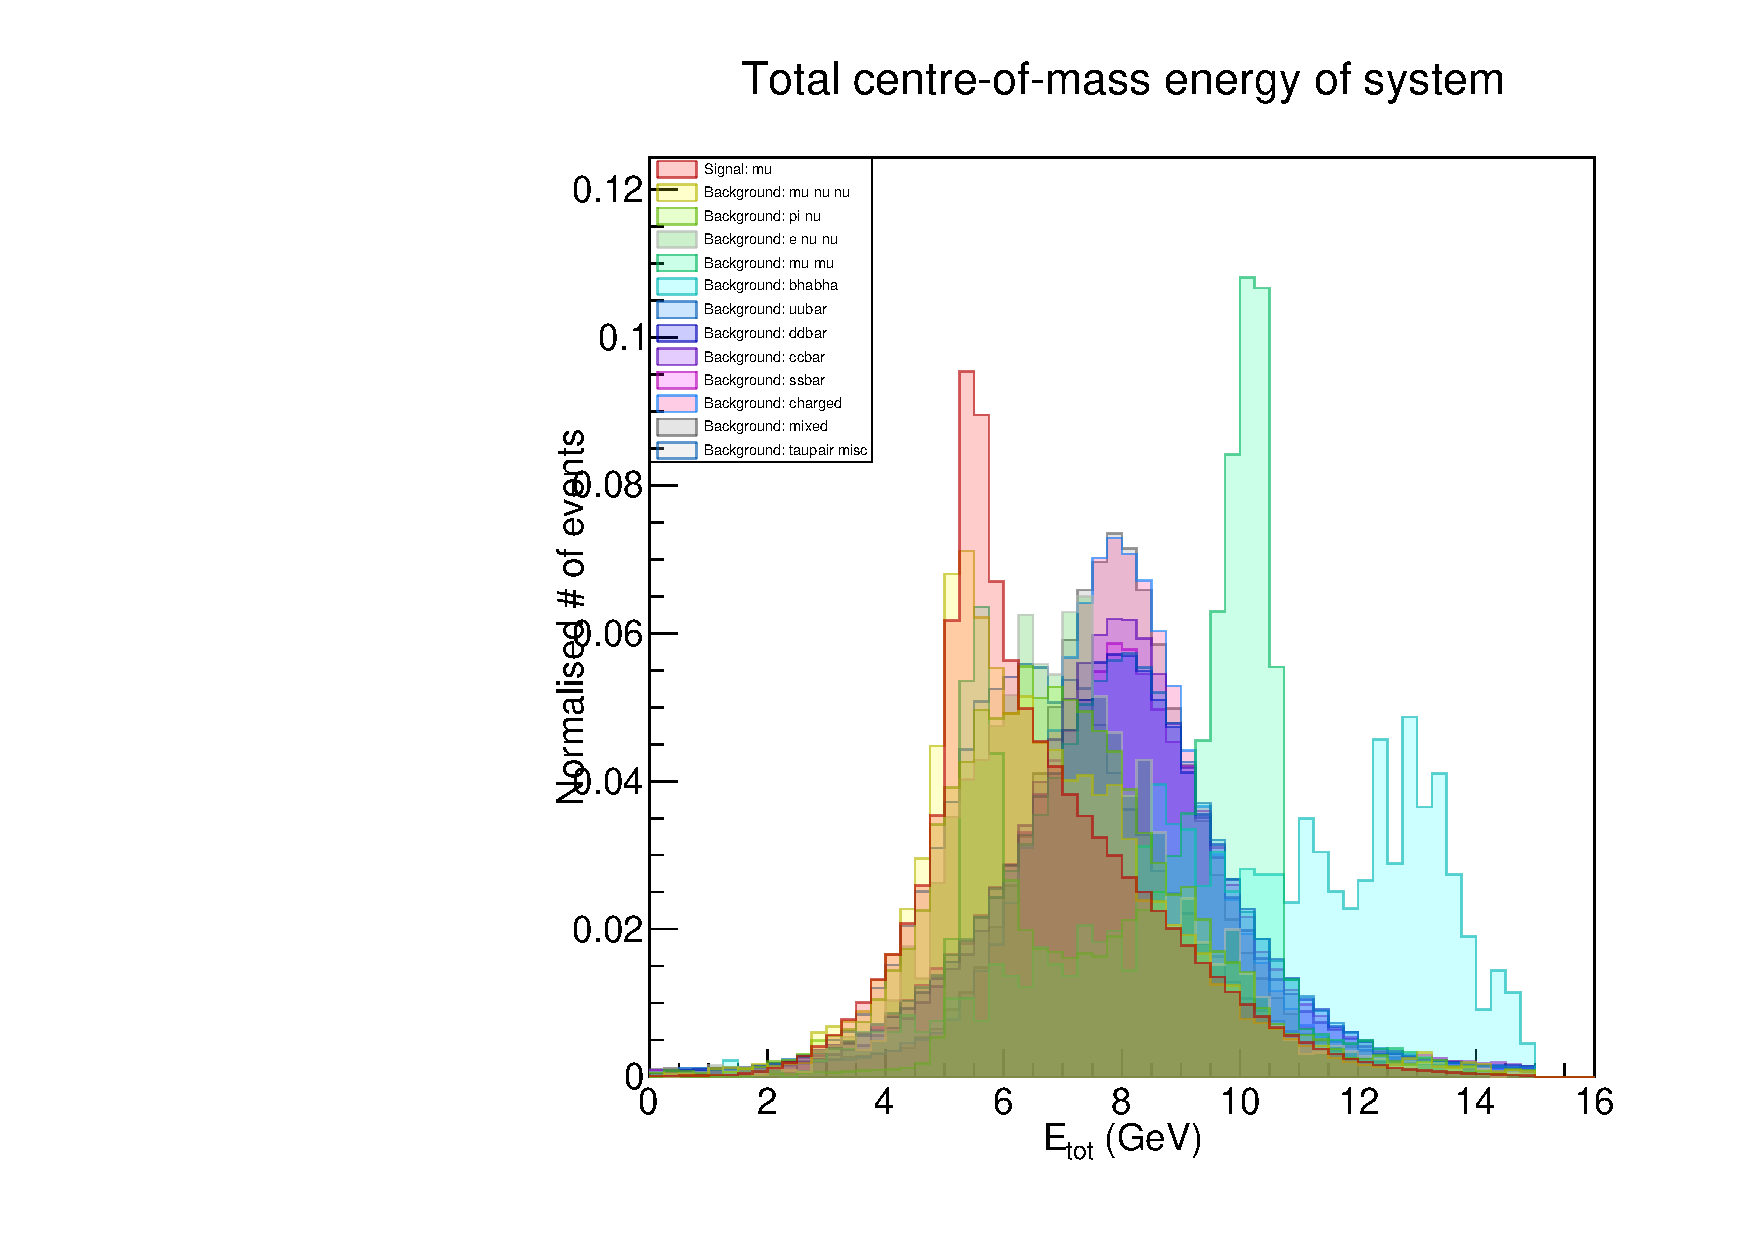
\includegraphics[width=\linewidth]{images/stack/stack_cut6_totalCM_E.pdf}
  \captionof{figure}{Another figure}
  \label{fig:test2}
\end{minipage}
\end{figure}

\begin{figure}[h]
\centering
\begin{minipage}{.5\textwidth}
  \centering
  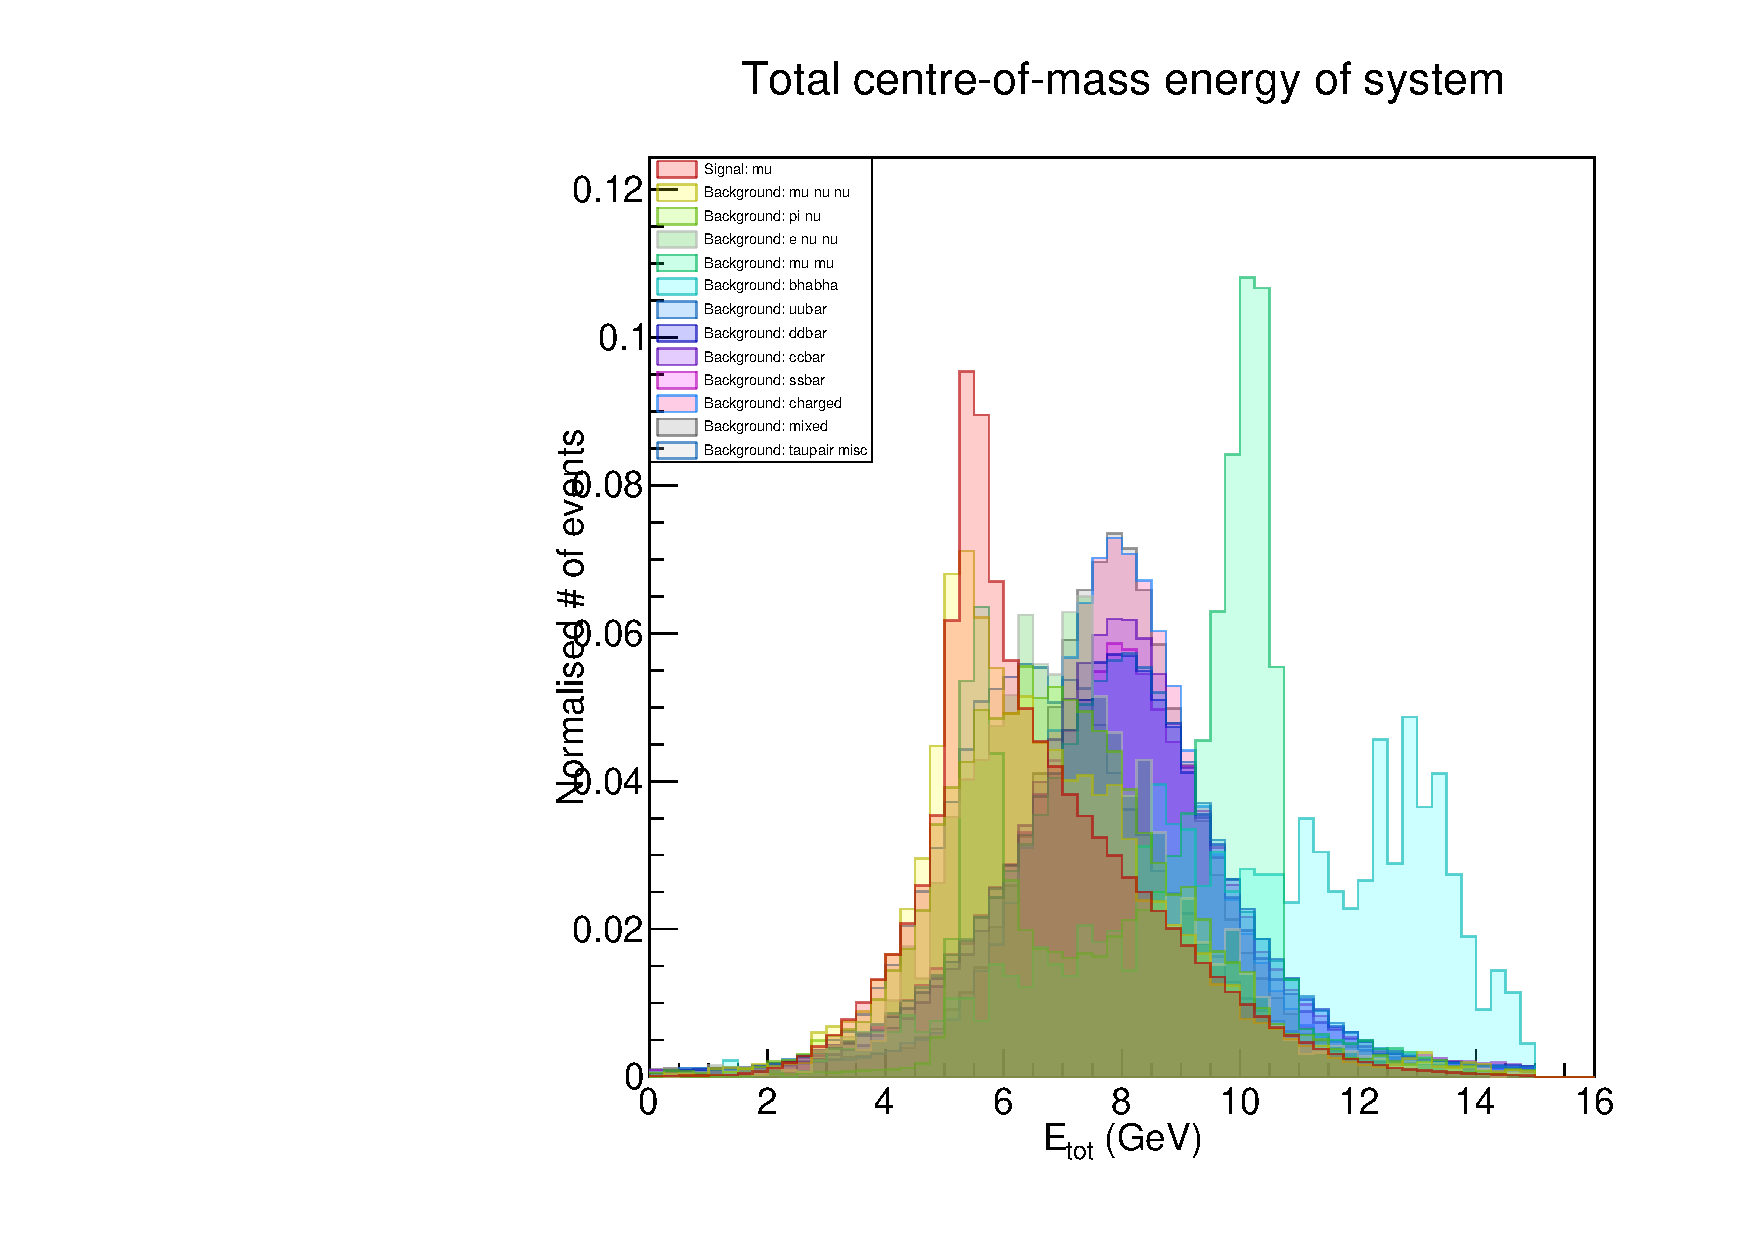
\includegraphics[width=\linewidth]{images/stack/stack_cut6_totalCM_E.pdf}
  \captionof{figure}{A figure}
  \label{fig:test1}
\end{minipage}%
\begin{minipage}{.5\textwidth}
  \centering
  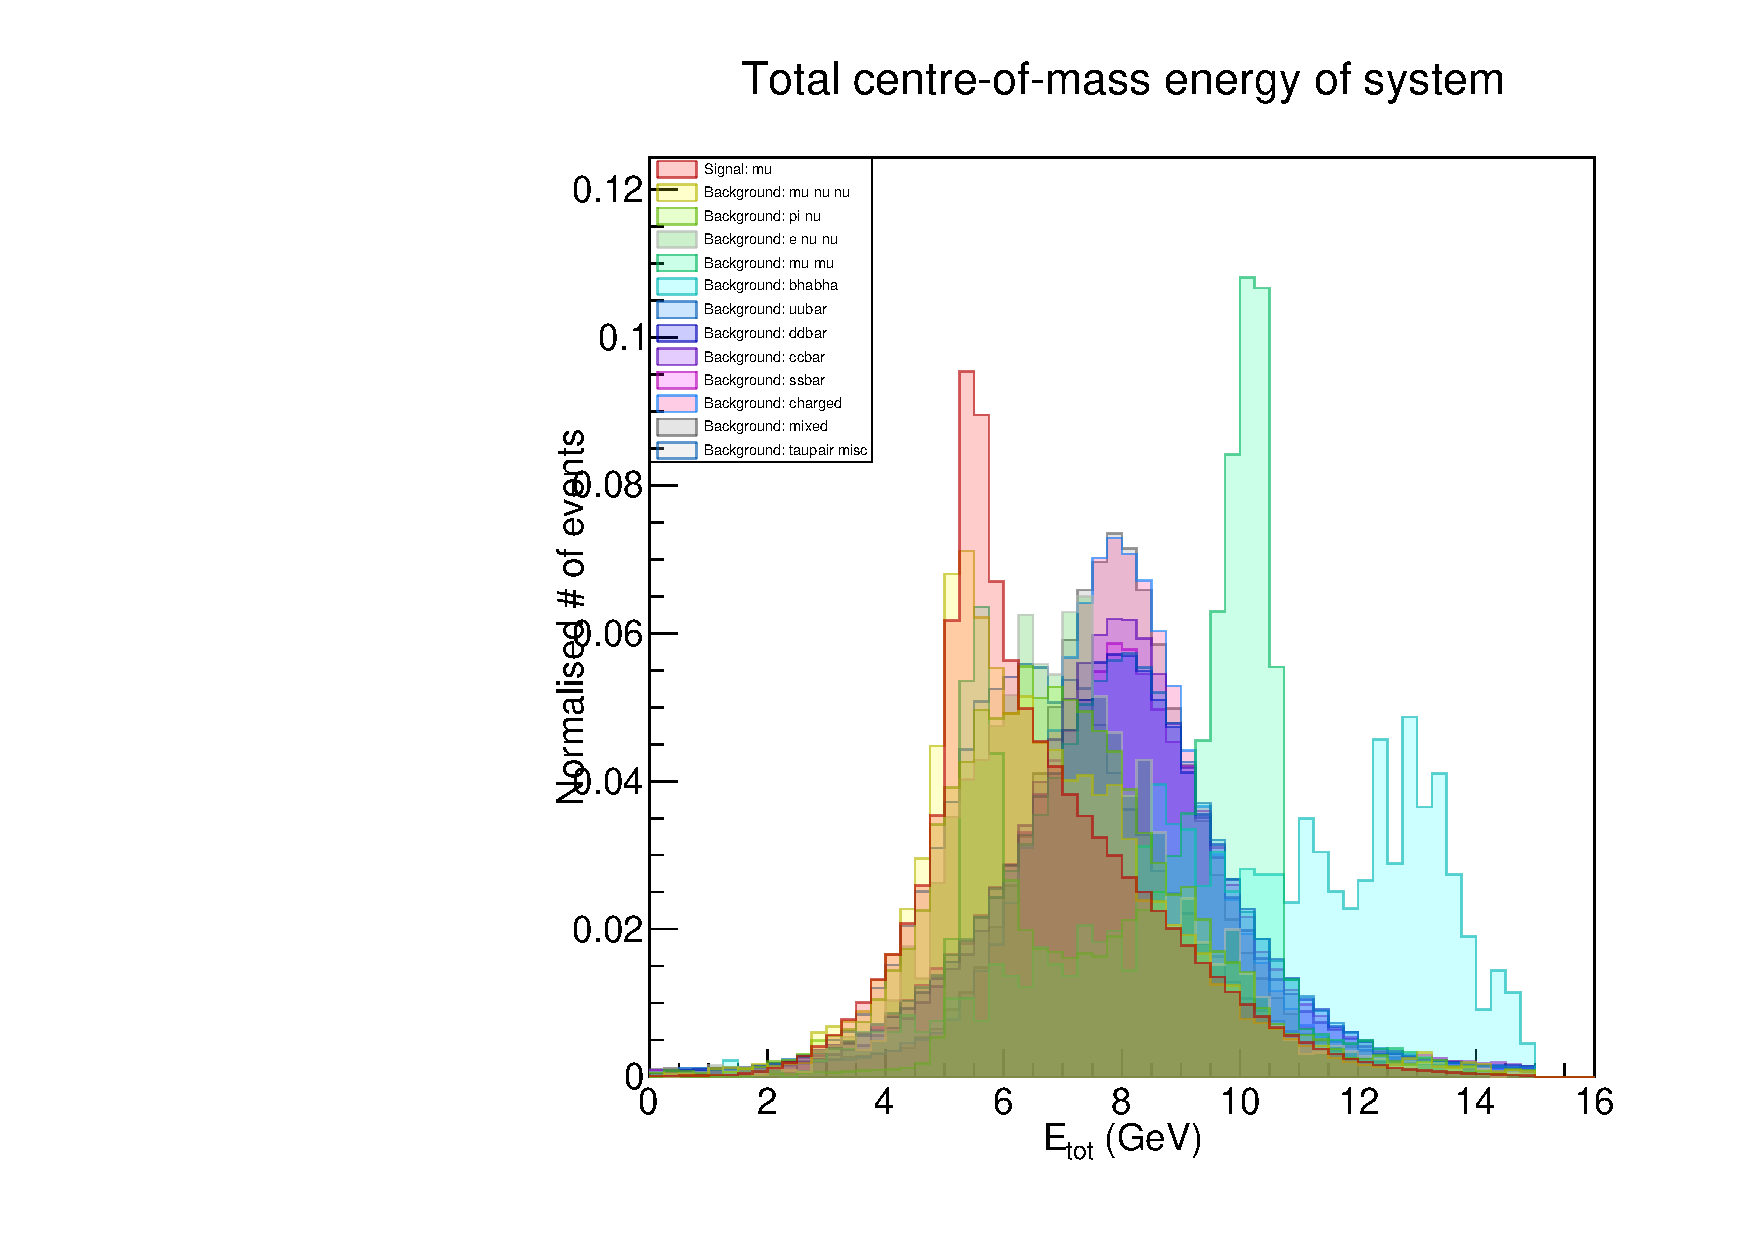
\includegraphics[width=\linewidth]{images/stack/stack_cut6_totalCM_E.pdf}
  \captionof{figure}{Another figure}
  \label{fig:test2}
\end{minipage}
\end{figure}


\pagebreak

\section{Backgrounds}

\subsection{Tau-pair processes}

A key difference between tau-pair backgrounds and the signal modes investigated is the lack of signal-side photon, and the existence of signal-side neutrinos.

We discuss the dominant tau-pair backgrounds $\tau\to e\nu\nu$, $\tau\to\mu\nu\nu$ and $\tau\to\pi\nu$ (where the pion is, of course, charged), with some minor discussion of the remaining modes. In tau-pair processes, the signal-side $\tau$ of energy $\SI{5.5}{GeV}$ decays dominantly into a single charged track and a neutrino (or neutrinos, in the pion modes). Light neutrinos carry away only a fraction of the energy from its mother particle; we expect the signal track to have a peak in energy of $\approx\SI{5.5}{GeV}$. However, the electron will lose a significant fraction of its energy due to bremsstrahlung as it passes through the detector and hence have a lower average energy. Signal track center-of-mass momentum is shown in Figure XXXXX below.

None of the dominant tau decay processes proceed with the final state photon; in most cases the reconstructed signal photon comes from initial state radiation (???? discuss this) or beam backgrounds. Photons produced as beam background are often low energy, especially compared to the average photon energy from signal processes of $\sim \SI{2.25}{GeV}$. Signal photon energy for tau-pair processes is shown in Figure XXXX; we note the peak energy of of $<\SI{1}{GeV}$. 

Since the signal photon does not originate from the signal-side $\tau$, the signal tracks appears ``boosted'' by comparison. This ``boost'' leads to the signal track and signal photon travelling almost back-to-back in the center-of-mass frame, in contrast to the signal mode where these final state particles have only a small opening angle between them.  


Since the signal track originates from the signal-side $\tau$ and is hence boosted in the center-of-mass frame by its mother particle,

Since this signal photon does not originate from the signal-side $\tau$, but instead from beam background or occasionally the tag-side $\tau$.

SOMETHING ABOUT E9E25.


\begin{figure}[h]
\centering
\begin{minipage}{.5\textwidth}
  \centering
  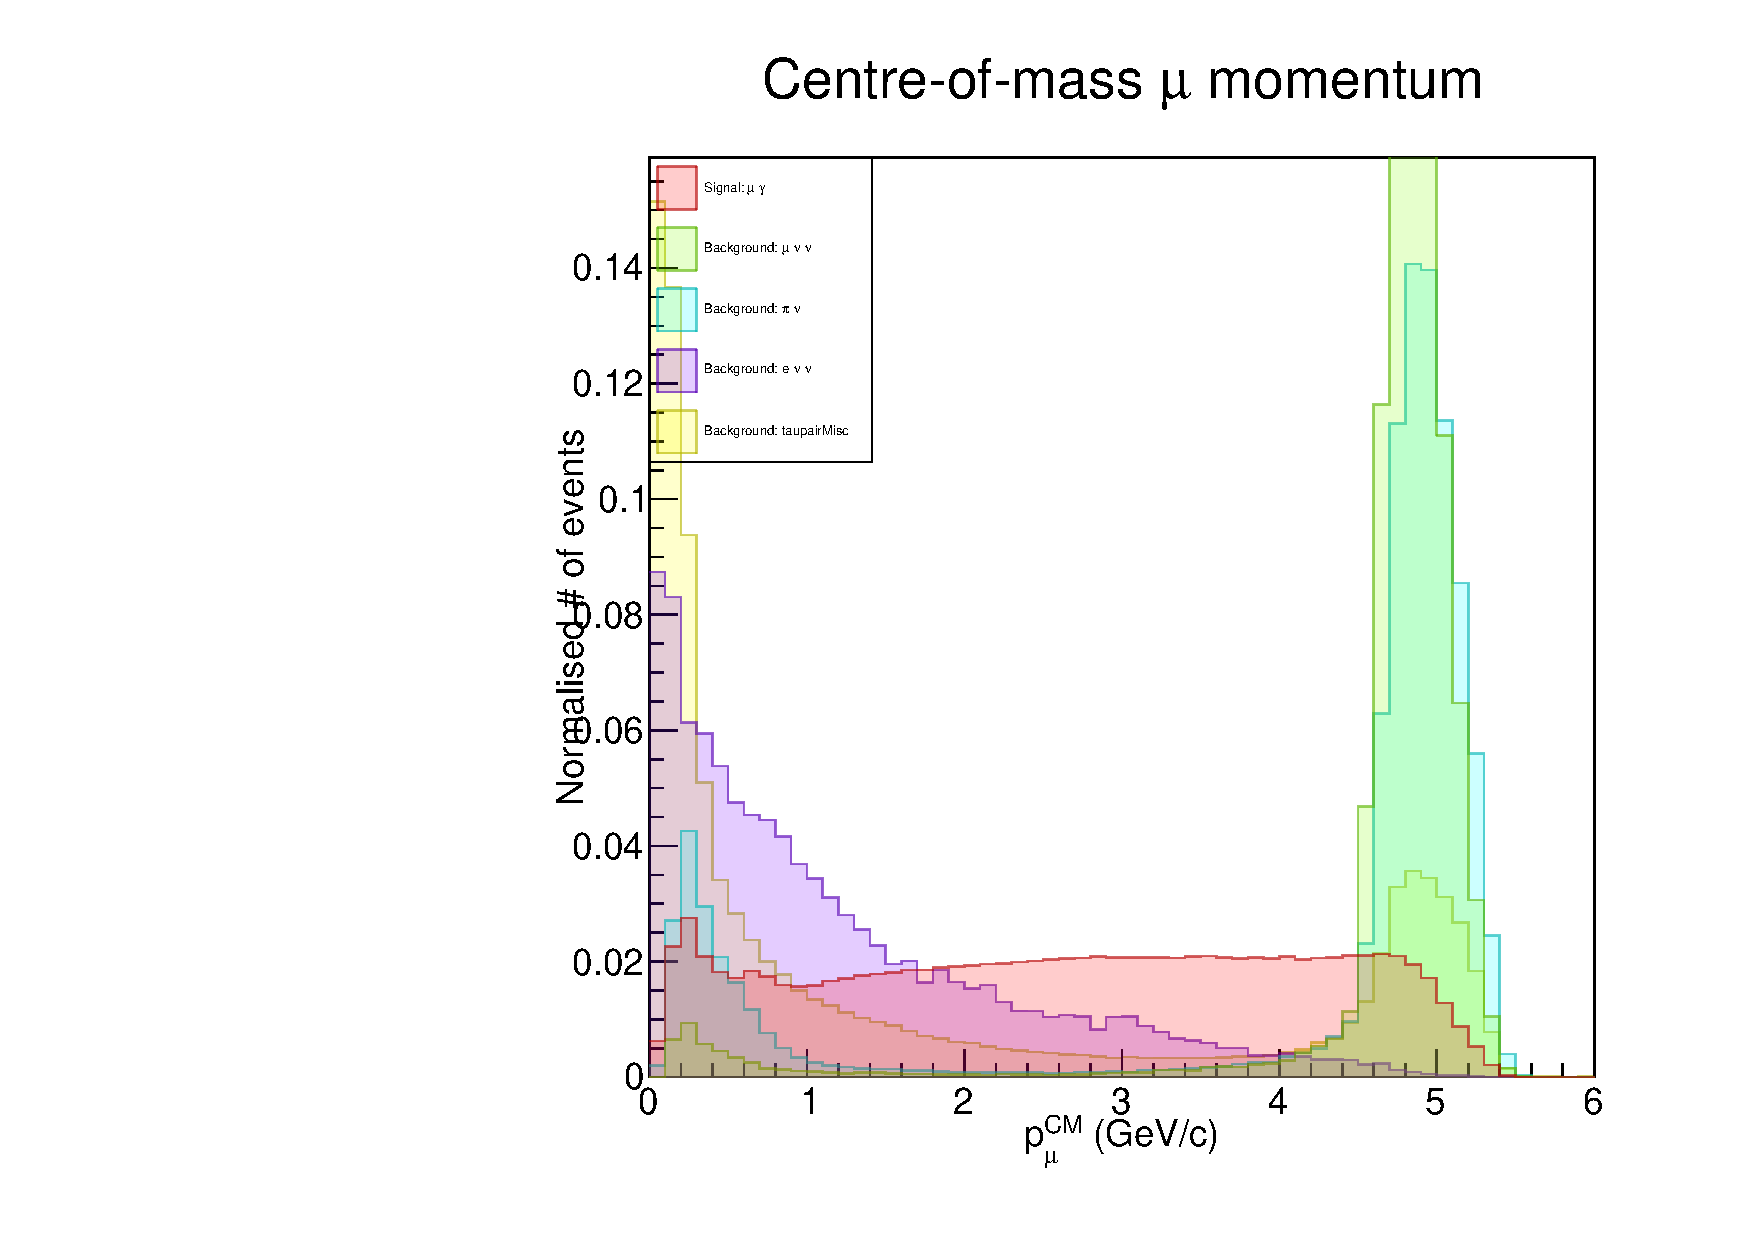
\includegraphics[width=\linewidth]{images/taupair-muCM_P.pdf}
  \captionof{figure}{Taupair - muCM P}
  \label{fig:test1}
\end{minipage}%
\begin{minipage}{.5\textwidth}
  \centering
  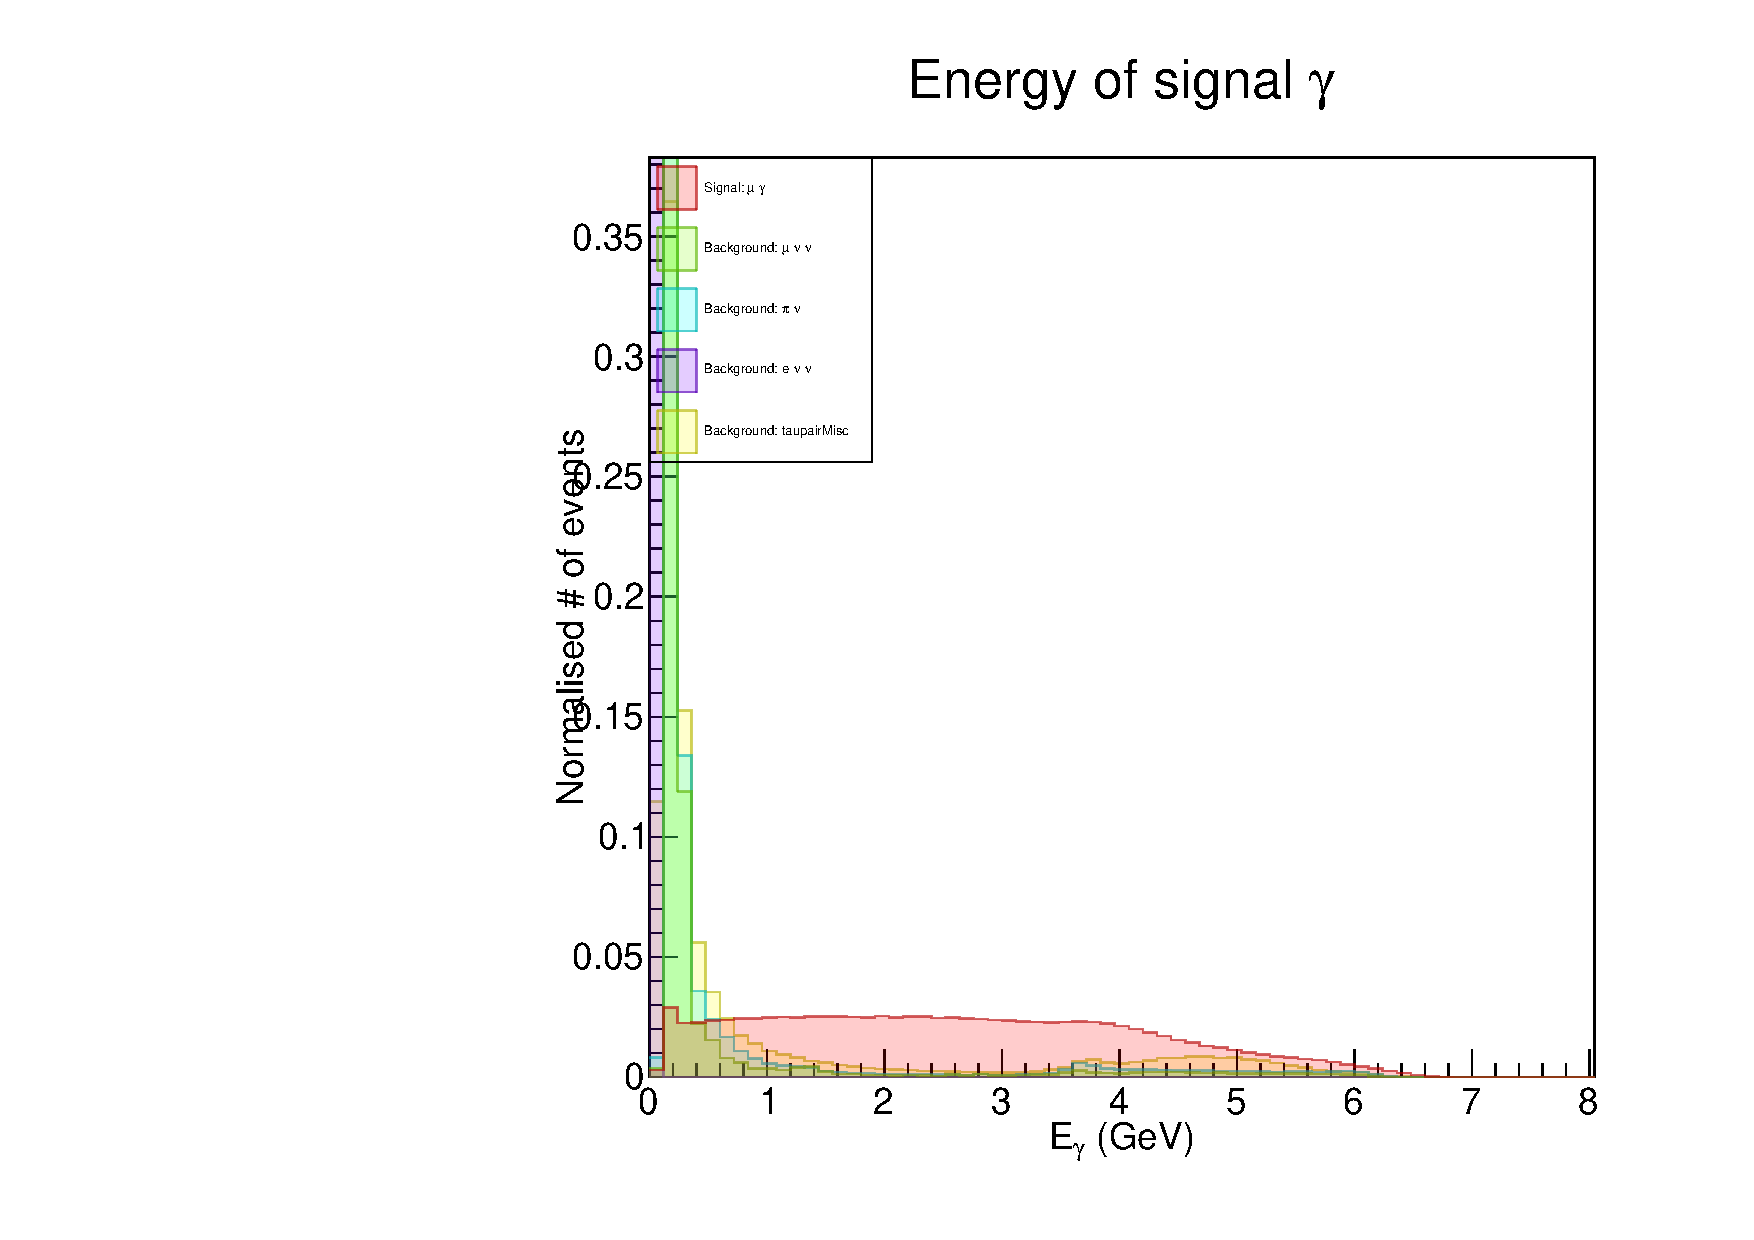
\includegraphics[width=\linewidth]{images/taupair-gamma_E.pdf}
  \captionof{figure}{Taupair - gamma E}
  \label{fig:test2}
\end{minipage}
\end{figure}

\begin{figure}[h]
\centering
\begin{minipage}{.5\textwidth}
  \centering
  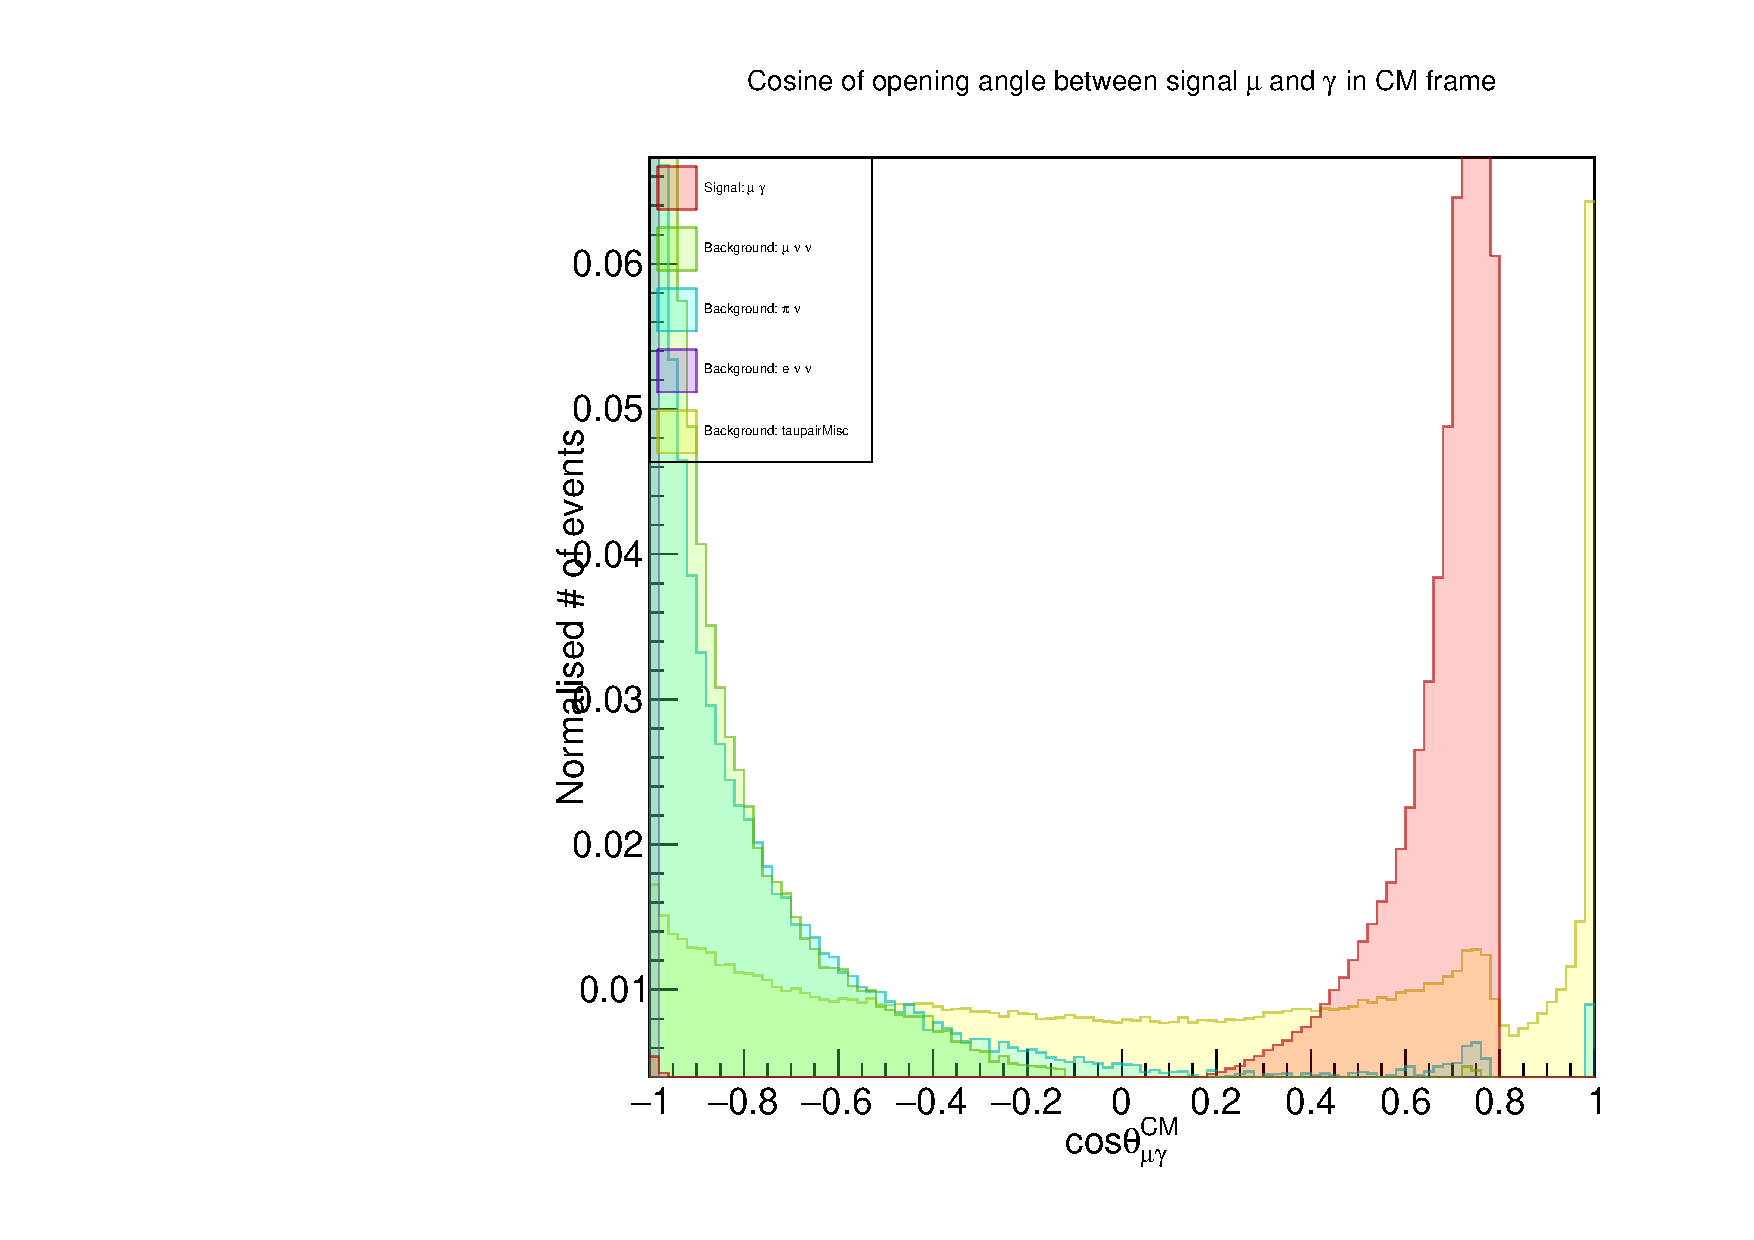
\includegraphics[width=\linewidth]{images/taupair-muGammaOpeningCM.pdf}
  \captionof{figure}{Taupair - muGammaOpeningCosThetaCM}
  \label{fig:test1}
\end{minipage}%
\begin{minipage}{.5\textwidth}
  \centering
  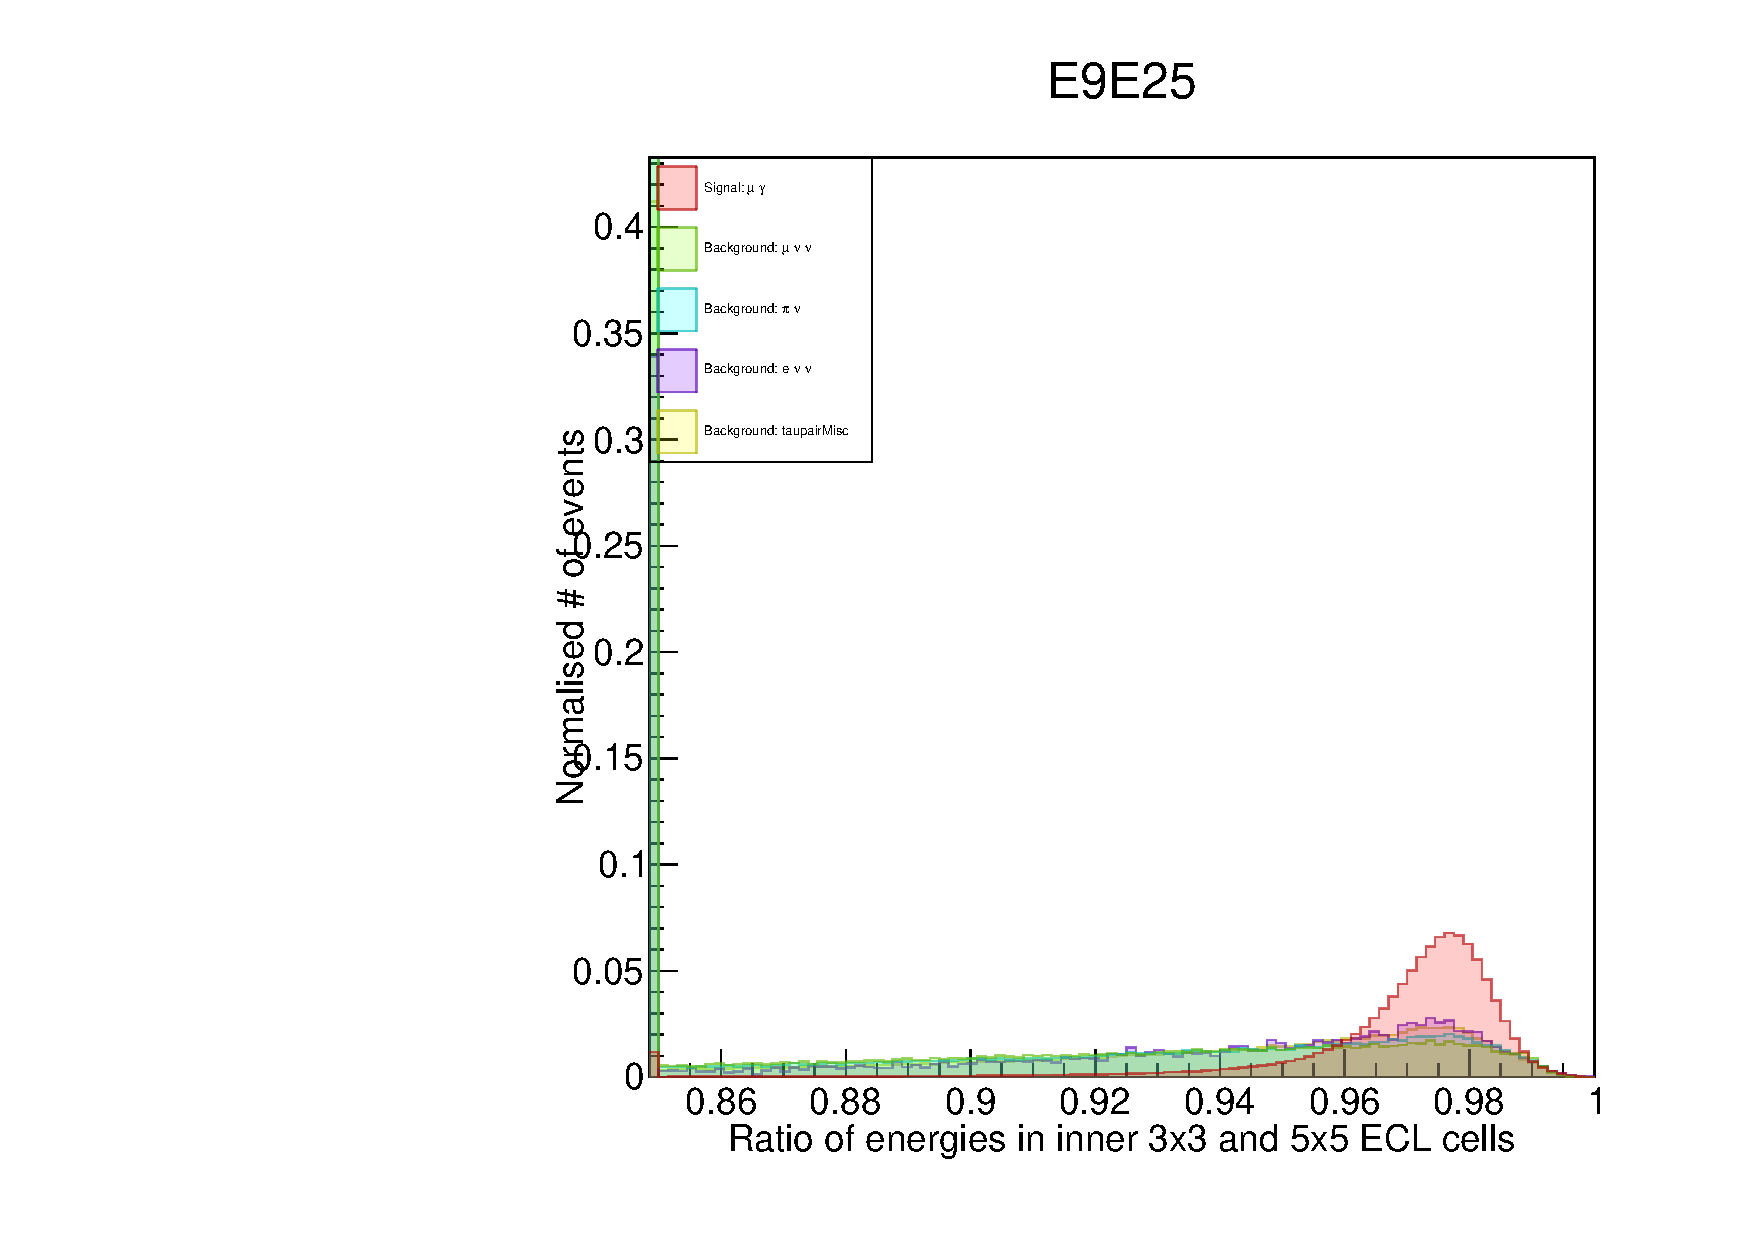
\includegraphics[width=\linewidth]{images/taupair-e9e25.pdf}
  \captionof{figure}{Taupair -E9E25}
  \label{fig:test2}
\end{minipage}
\end{figure}


\subsection{Mu-pair processes}

Muons are very cleanly reconstructed by the detector; they do not lose any significant amount of energy through bremsstrahlung radiation, and they penetrate deeply leaving a distinct signal. Unlike the tau-pair processes or the signal modes discussed above, mu-pair processes $e^+ e^- \to \mu^+ \mu^- (\gamma)$, both signal- and tag-side channels consist of only a single charged track each, sometimes with a final state photon. Hence, mu-pair processes are reconstructed very well. This is evidenced by the majority of events with only two reconstructed tracks (see Figure XXXX); this is is stark comparison to the spread of tracks from two up to fifteen in tau-pair events. Total reconstructed energy peaks around $\SI{10.5}{GeV}$.

By momentum conservation, the signal and tag tracks are generated back-to-back for $\mu\mu$ final states (XXX \% of all mu-pair processes), or with an opening angle similar to the signal mode for $\mu\mu\gamma$ final states (XXXX \% of all mu-pair processes). The signal photon is often reconstructed from low energy beam background photons, as with background tau-pair processes. A similar photon energy spectrum can be seen in Figure XXXX.

MORE TOPOLOGY STUFF?

\begin{figure}[h]
\centering
\begin{minipage}{.5\textwidth}
  \centering
  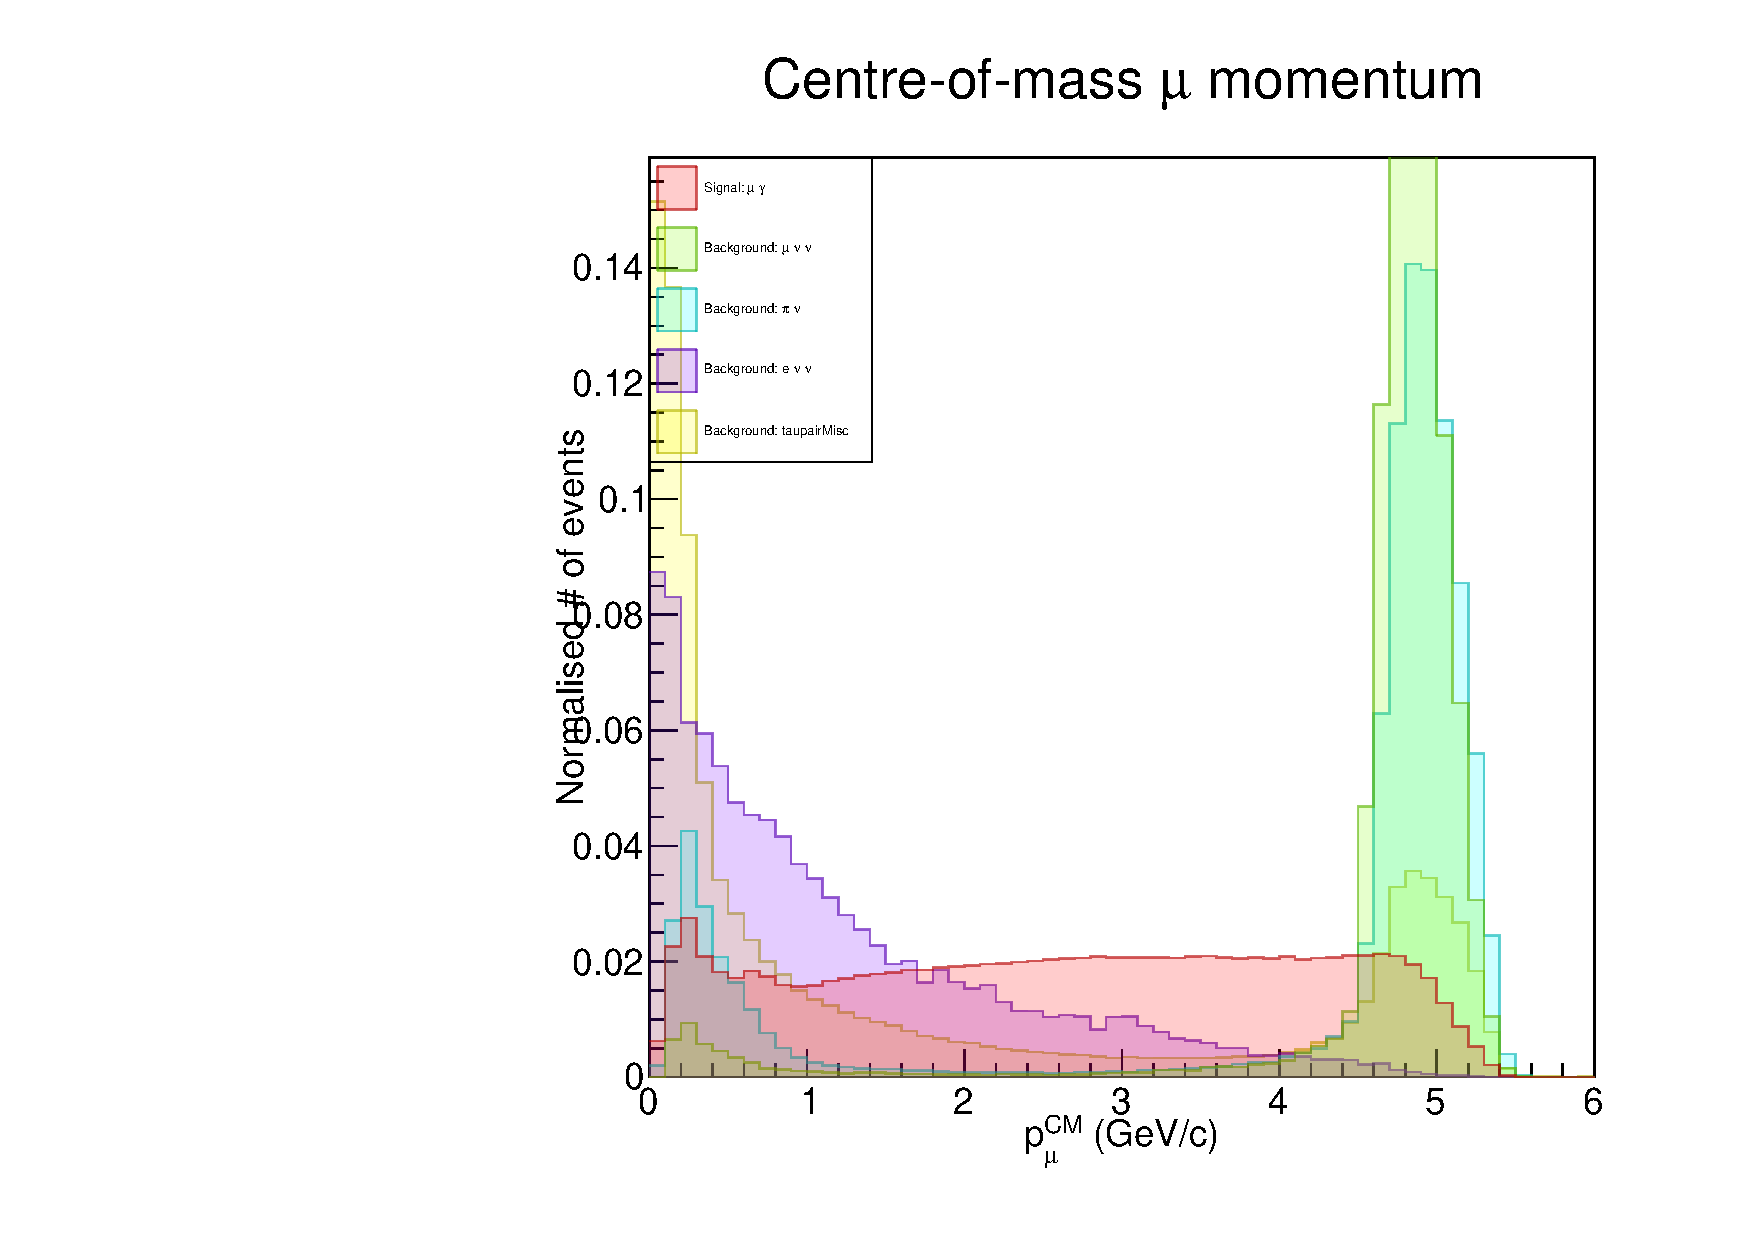
\includegraphics[width=\linewidth]{images/taupair-muCM_P.pdf}
  \captionof{figure}{Taupair - muCM P}
  \label{fig:test1}
\end{minipage}%
\begin{minipage}{.5\textwidth}
  \centering
  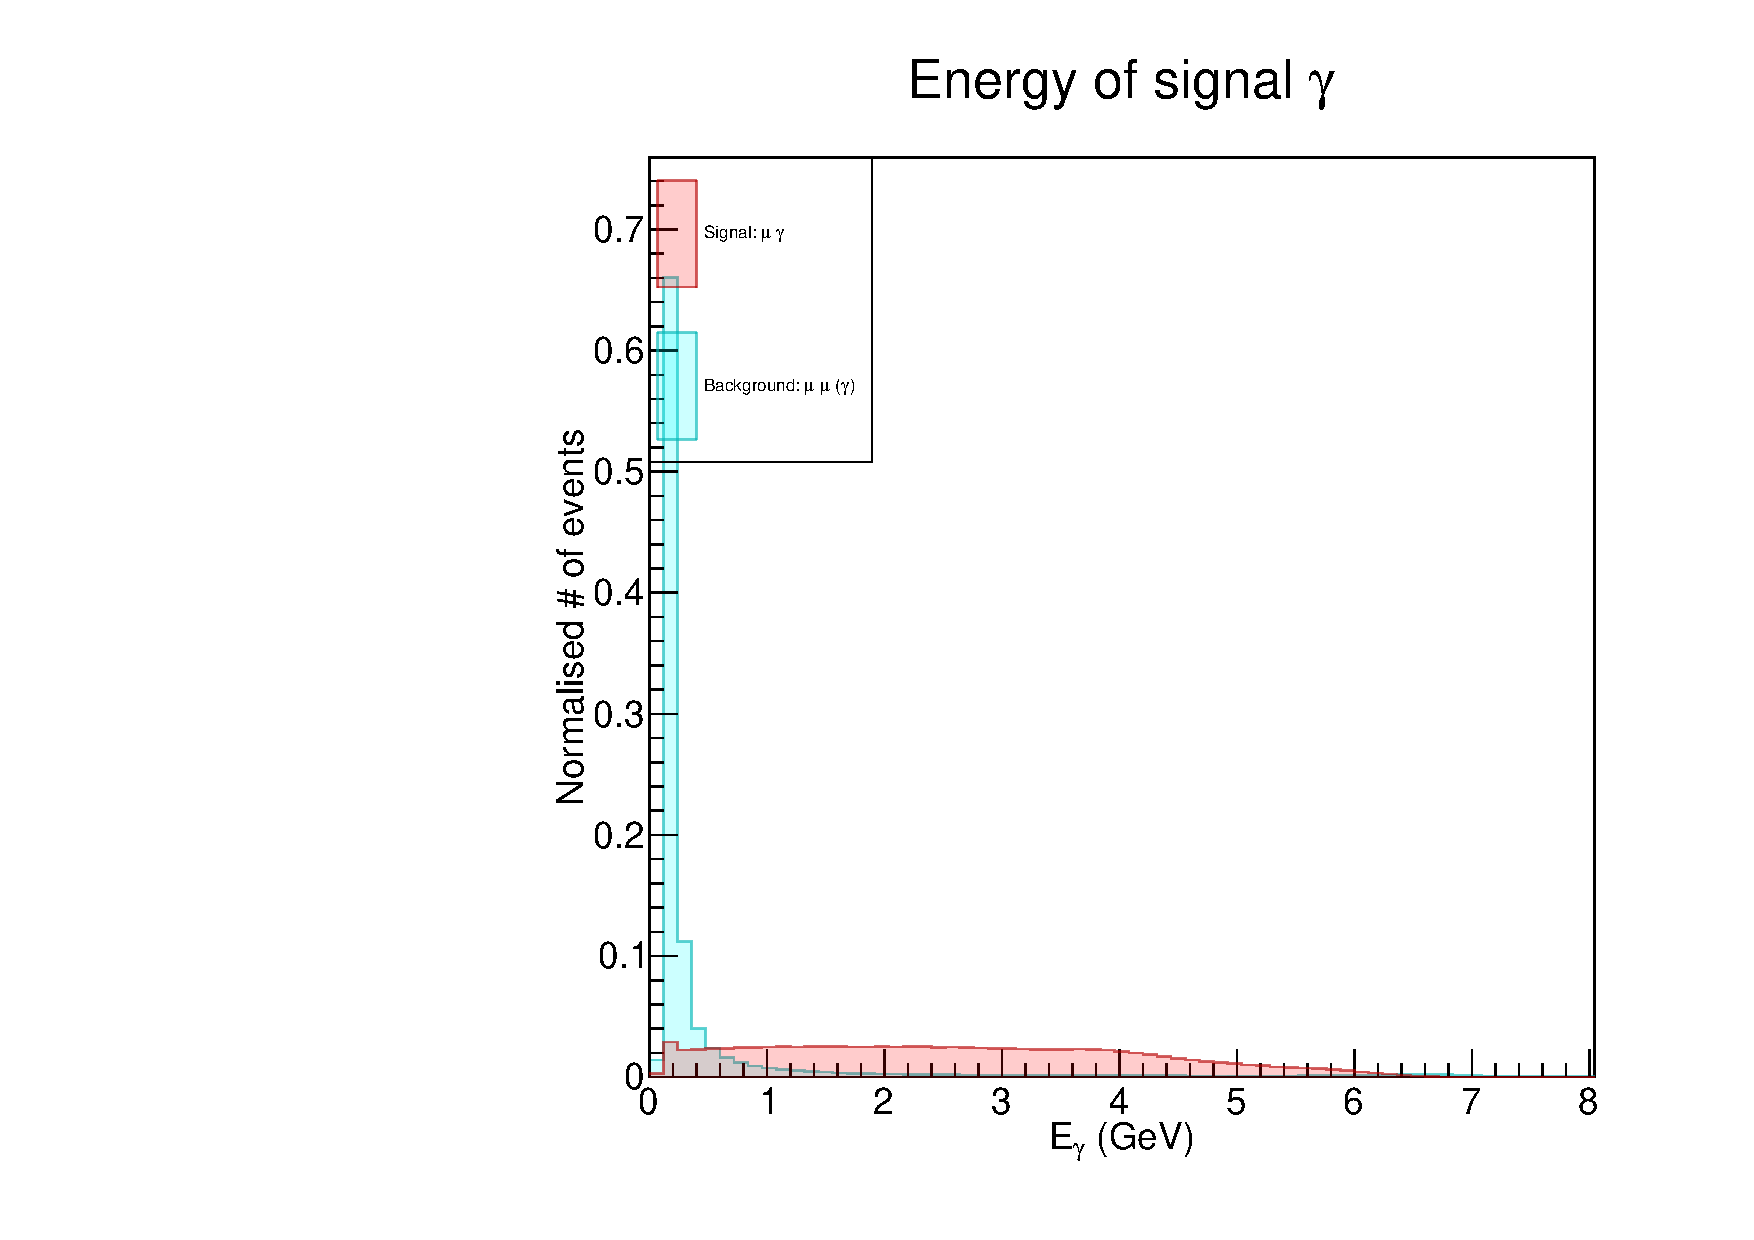
\includegraphics[width=\linewidth]{images/mupair-gamma_E.pdf}
  \captionof{figure}{Mu-pair: gamma E}
  \label{fig:test2}
\end{minipage}
\end{figure}

\begin{figure}[h]
\centering
\begin{minipage}{.5\textwidth}
  \centering
  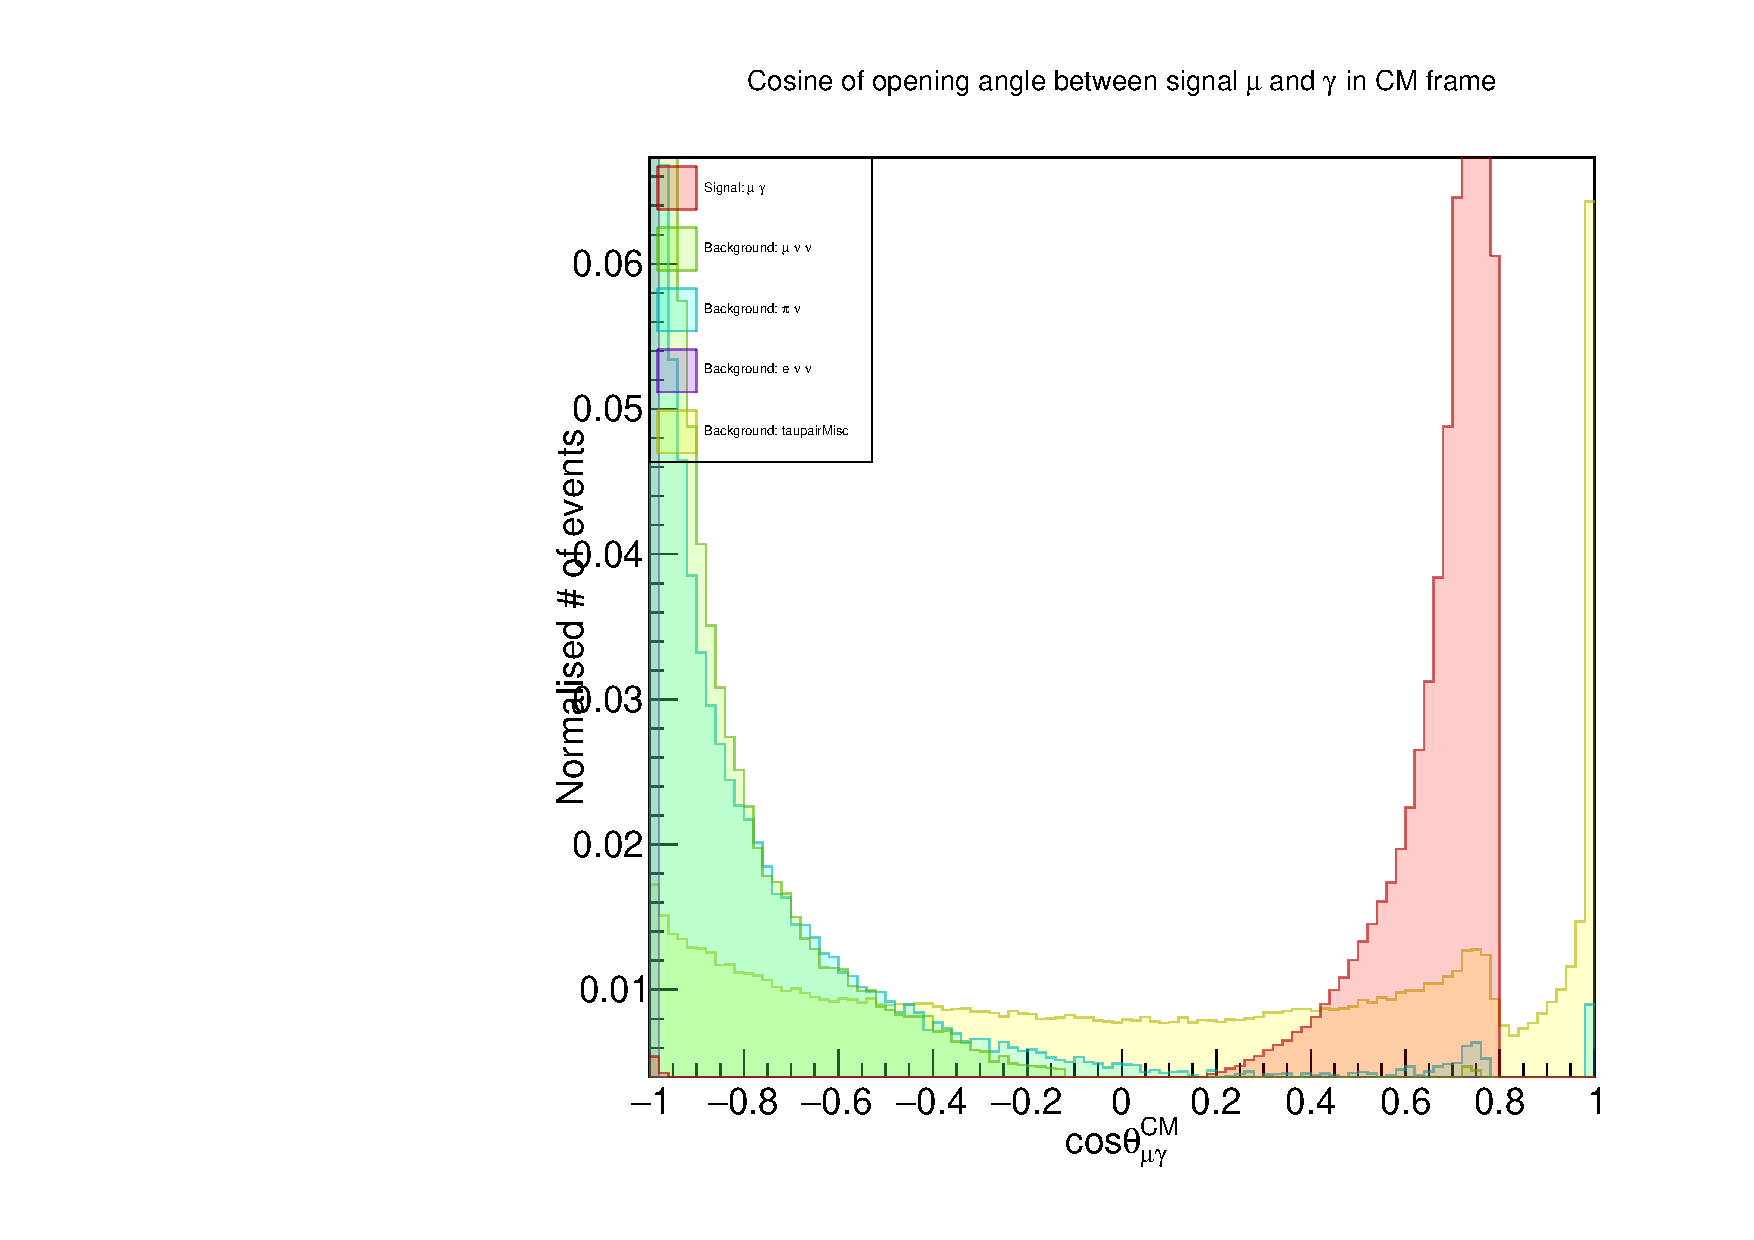
\includegraphics[width=\linewidth]{images/taupair-muGammaOpeningCM.pdf}
  \captionof{figure}{Taupair - muGammaOpeningCosThetaCM}
  \label{fig:test1}
\end{minipage}%
\begin{minipage}{.5\textwidth}
  \centering
  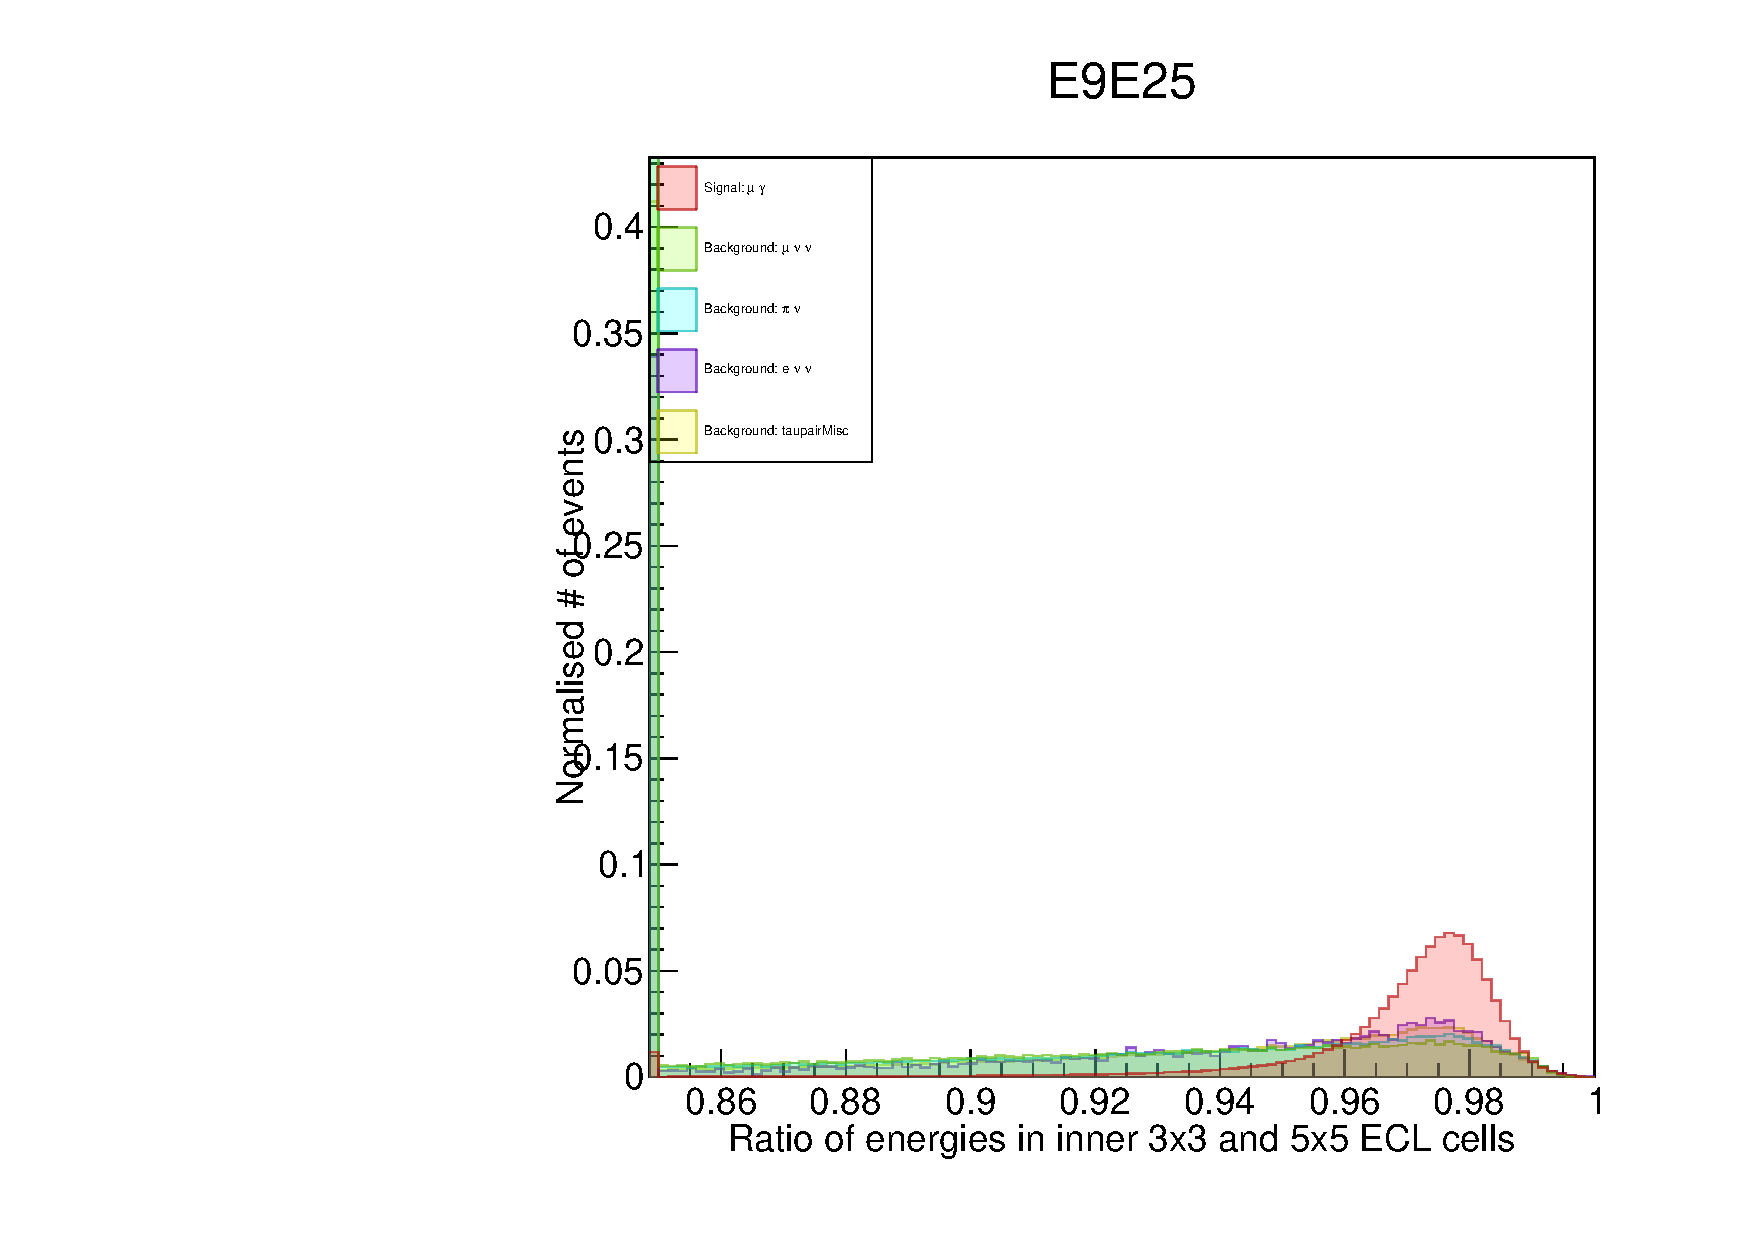
\includegraphics[width=\linewidth]{images/taupair-e9e25.pdf}
  \captionof{figure}{Taupair -E9E25}
  \label{fig:test2}
\end{minipage}
\end{figure}



\subsection{Bhabha}

Bhabha events $e^+ e^- \to e^+ e^- (\gamma)$ have event signatures (???) very similar to mu-pair processes $e^+ e^- \to \mu^+ \mu^- (\gamma)$, for obvious reasons. However, as is case with electrons in the detector, both signal and tag track particles lose a significant portion of their energy to bremsstrahlung and are not reconstructed as cleanly as muons. 

Smearing of energies and momenta occurs for bhabha event reconstruction, with measureables not peaking as strongly as for mu-pair events and instead spreading across a values. These features are shown in Figures XXX and XXX below, comparing distributions for mu-pair events to bhabha events. Much of the event topology is still common between these processes, however.

\begin{figure}[h]
\centering
\begin{minipage}{.5\textwidth}
  \centering
  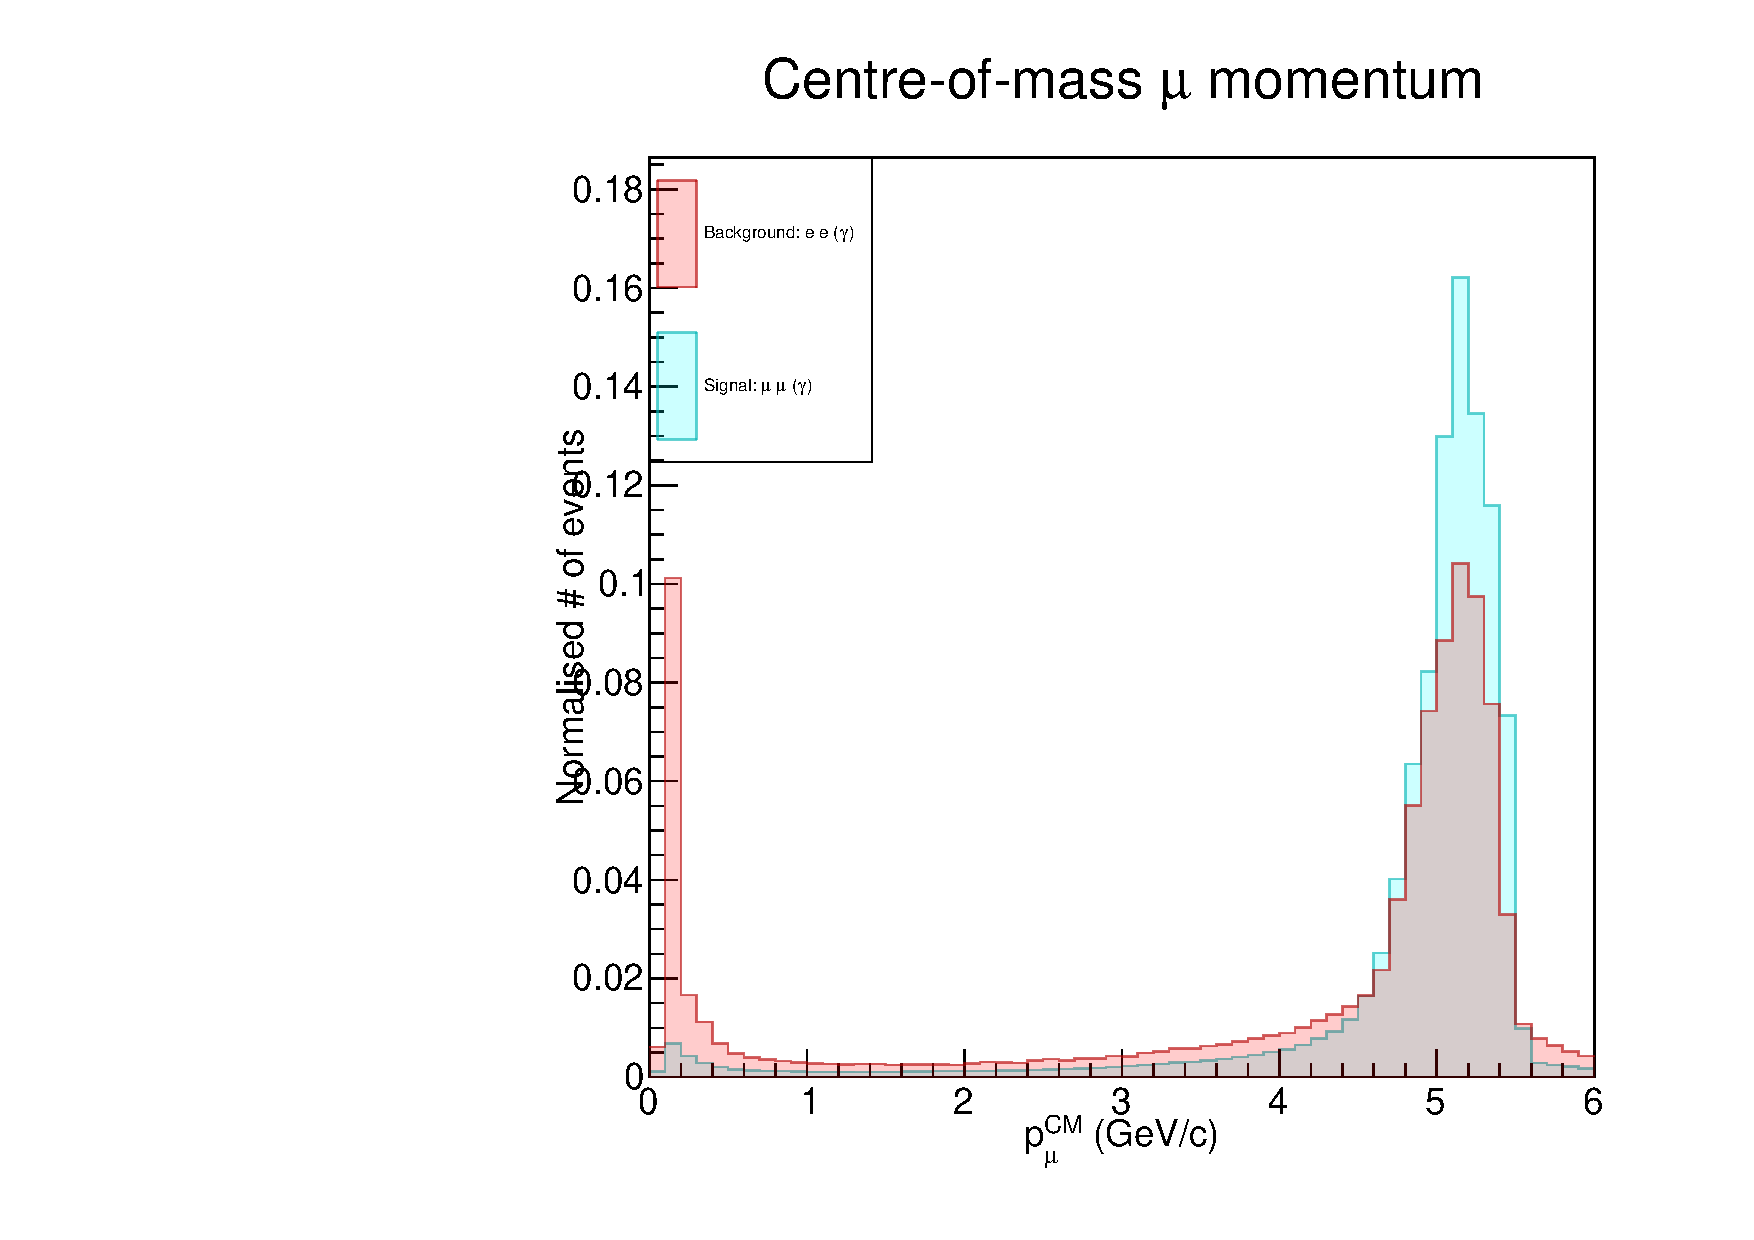
\includegraphics[width=\linewidth]{images/bhabha-mupair-muCM_P.pdf}
  \captionof{figure}{Bhabha: muCM P}
  \label{fig:test1}
\end{minipage}%
\begin{minipage}{.5\textwidth}
  \centering
  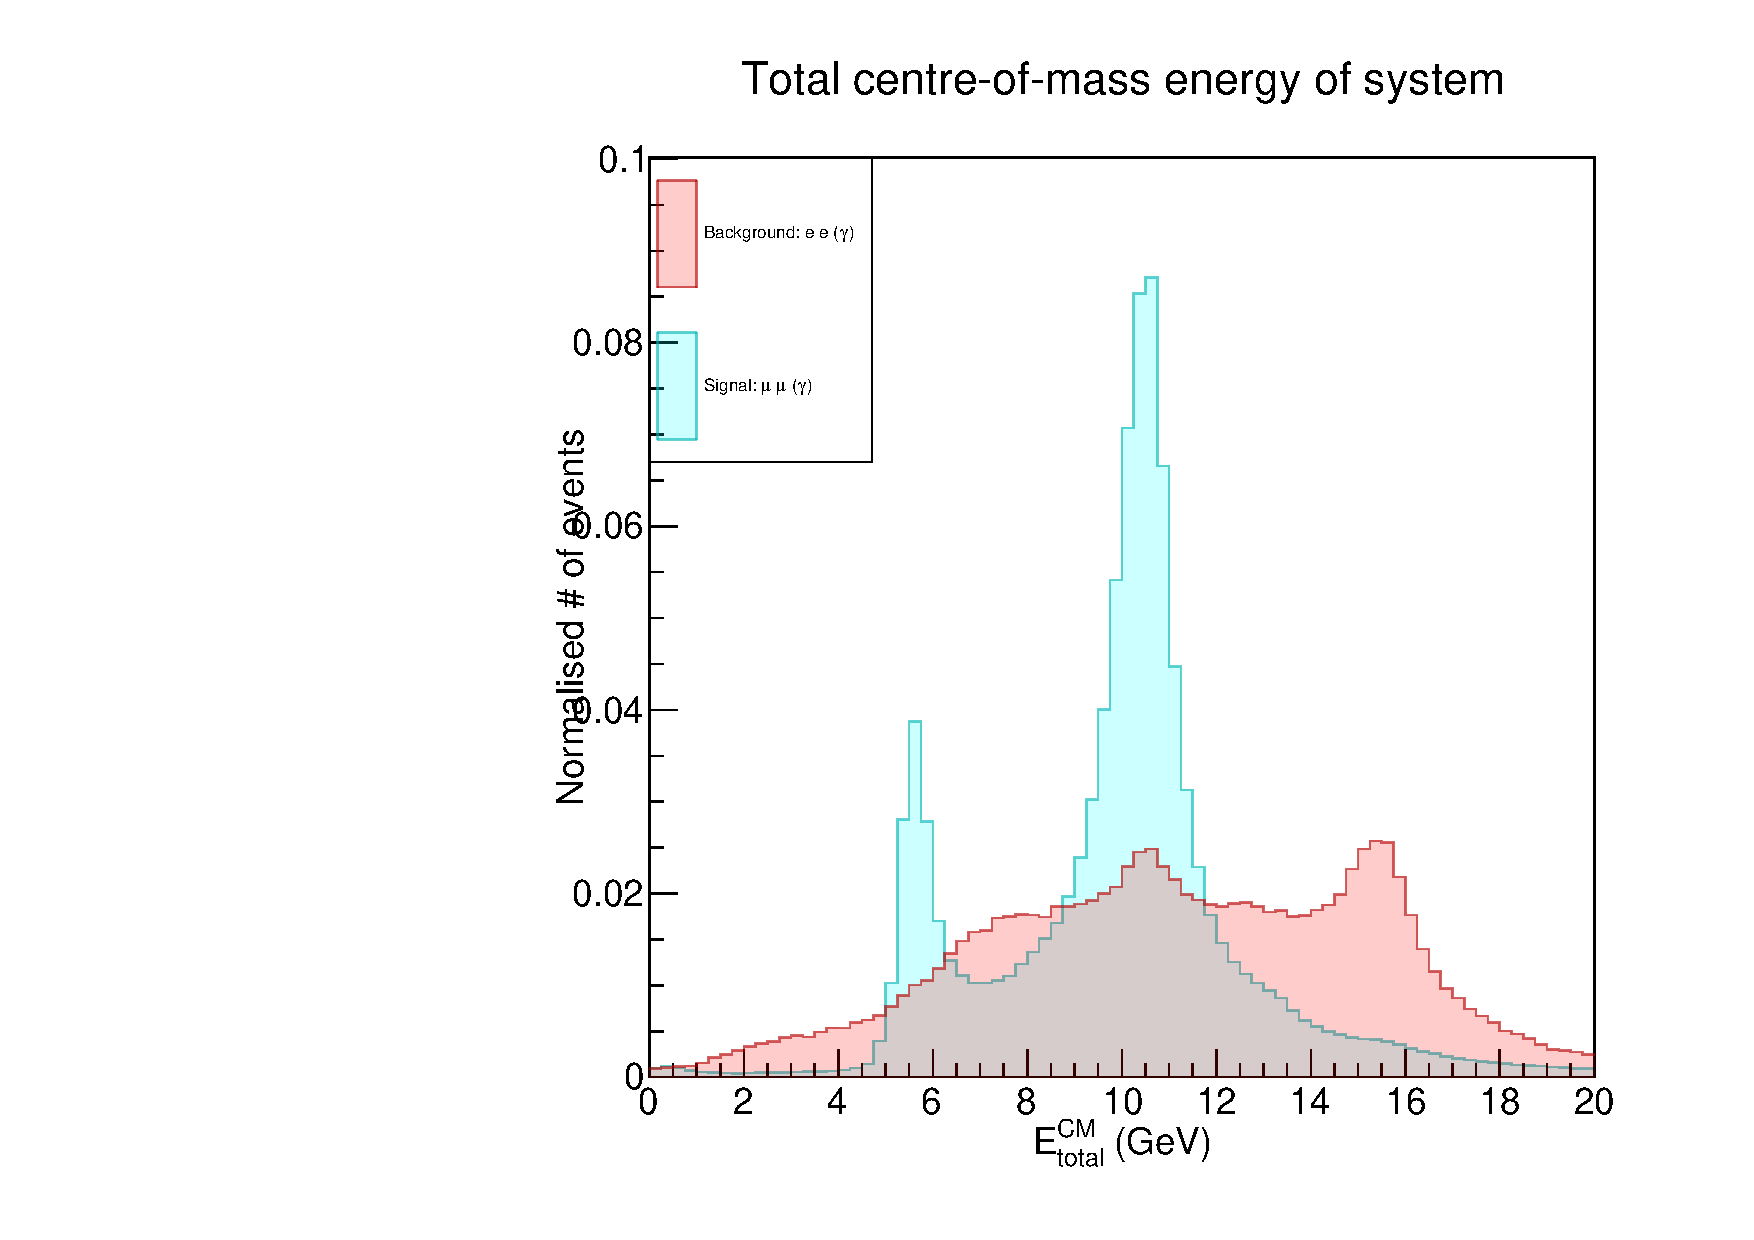
\includegraphics[width=\linewidth]{images/bhabha-mupair-totalCM_E.pdf}
  \captionof{figure}{Bhabha: totalCM E}
  \label{fig:test2}
\end{minipage}
\end{figure}


\subsection{Continuum and $B\bar{B}$}

NOT SURE HOW TO DESCRIBE TOPOLOGIES FOR THESE EVENTS


\begin{figure}[h]
\centering
\begin{minipage}{.5\textwidth}
  \centering
  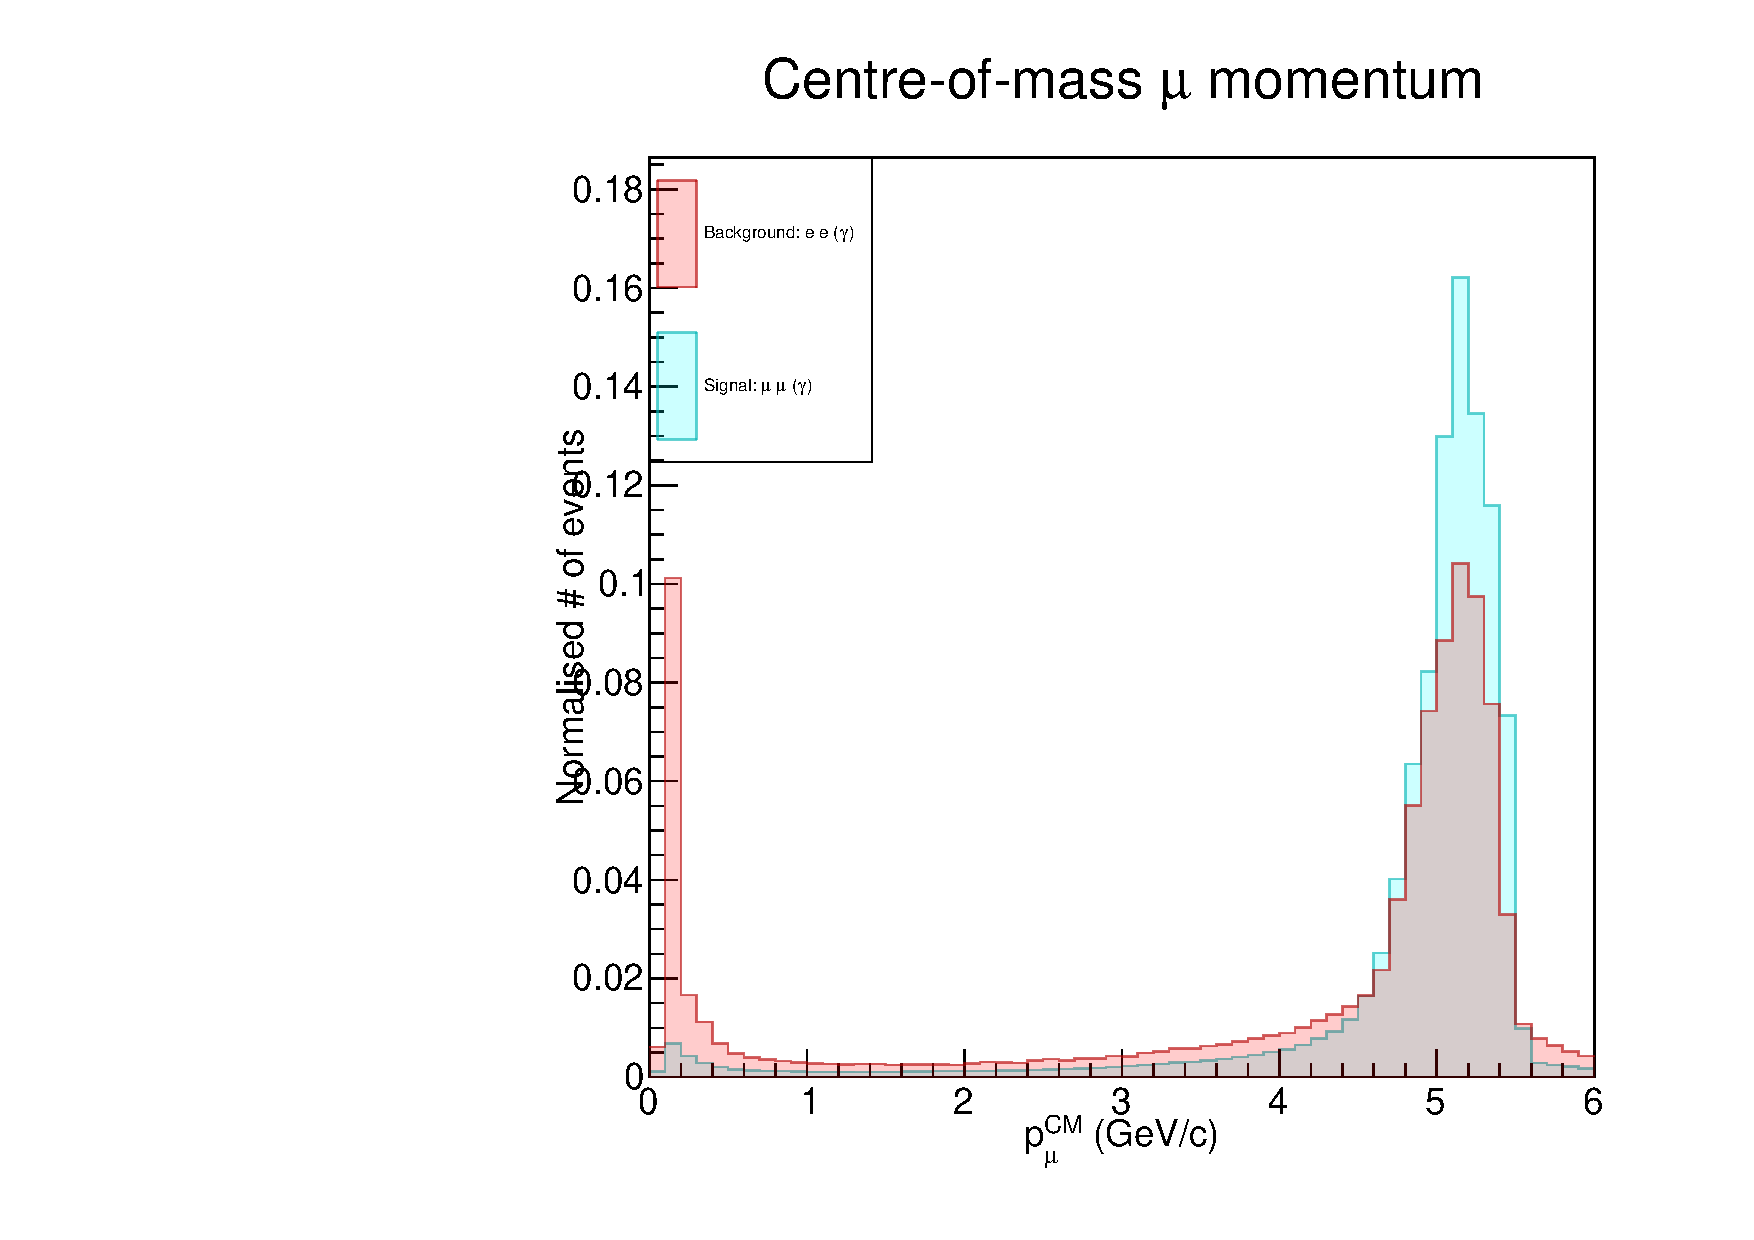
\includegraphics[width=\linewidth]{images/bhabha-mupair-muCM_P.pdf}
  \captionof{figure}{Bhabha: muCM P}
  \label{fig:test1}
\end{minipage}%
\begin{minipage}{.5\textwidth}
  \centering
  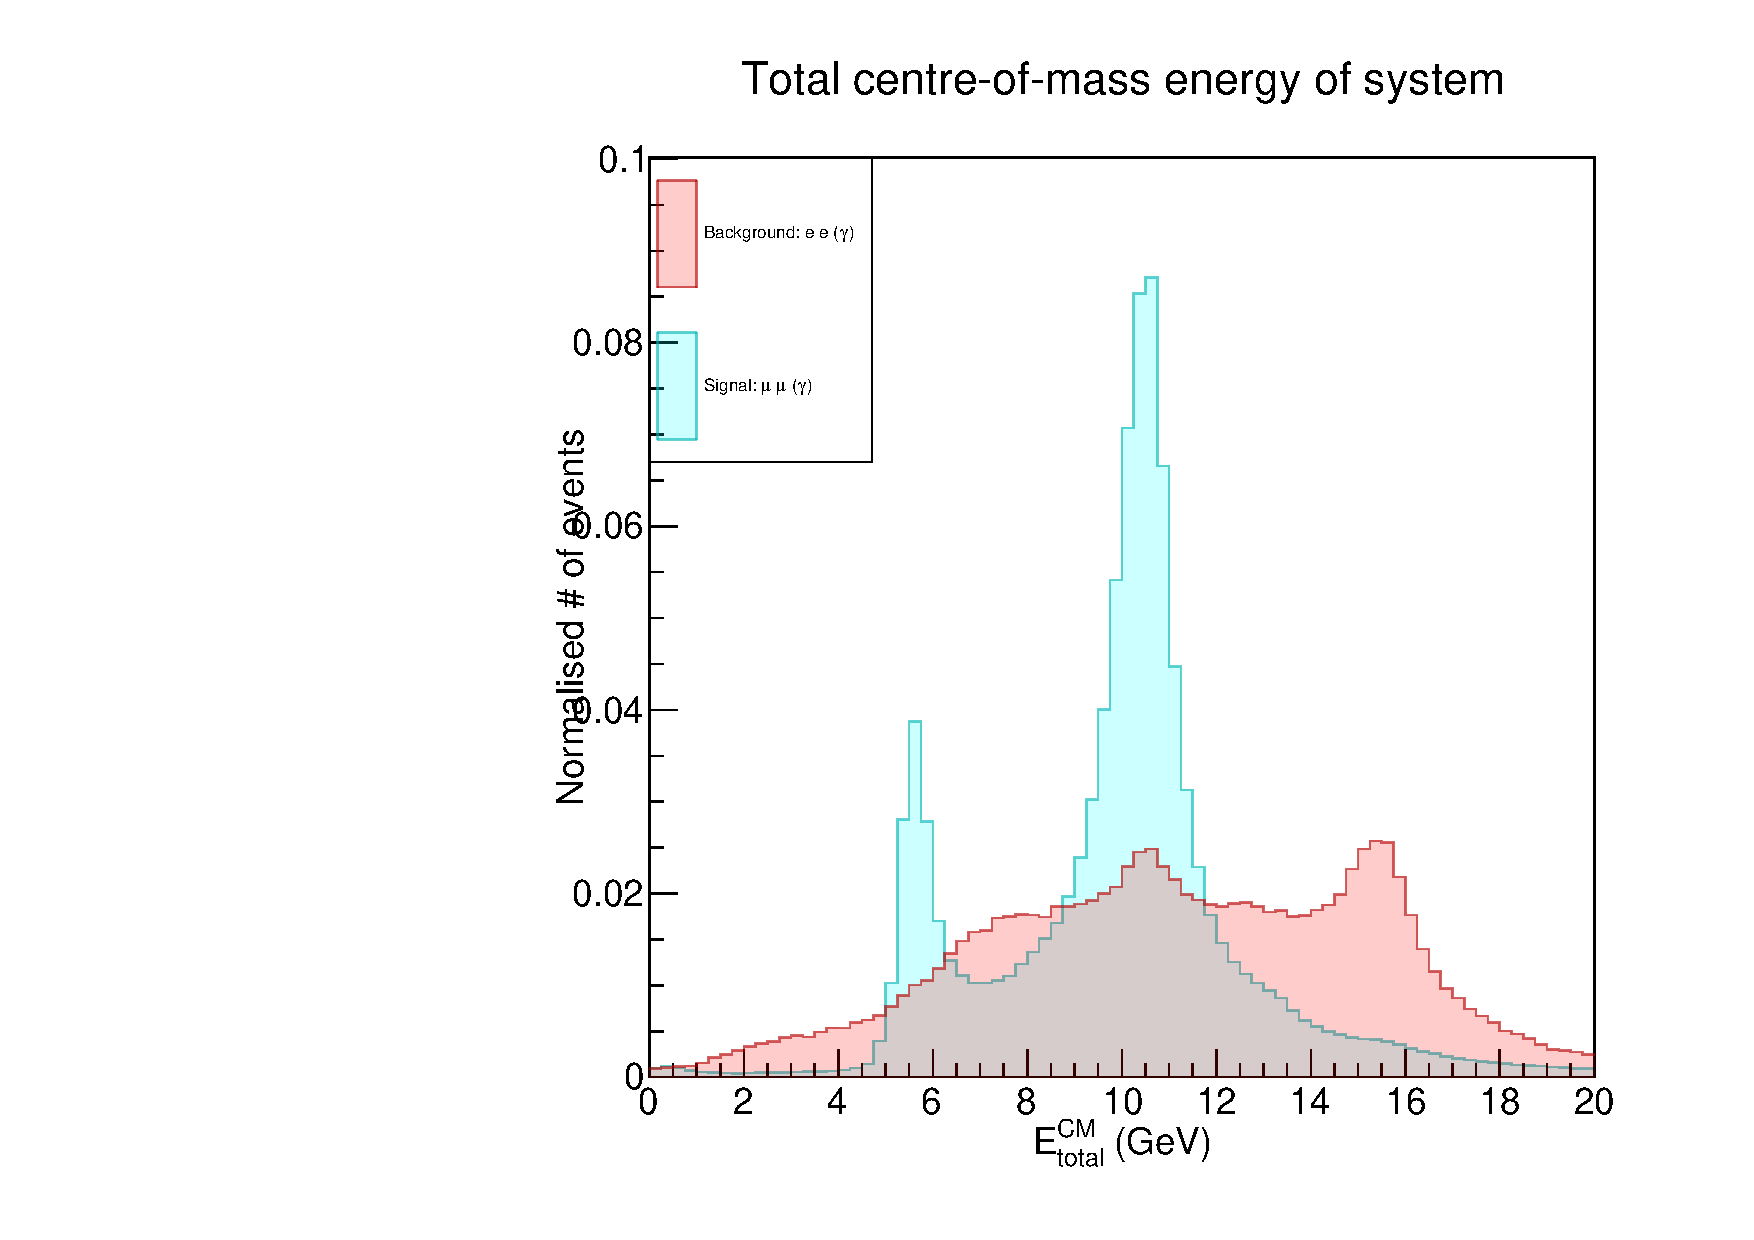
\includegraphics[width=\linewidth]{images/bhabha-mupair-totalCM_E.pdf}
  \captionof{figure}{Bhabha: totalCM E}
  \label{fig:test2}
\end{minipage}
\end{figure}



\pagebreak

%-------------------------------------------------------------------

\chapter{Preselection}

Following reconstruction, preselection criteria were applied to the reconstructed events. Preselection criteria are defined as distinct from selection criteria in that they remove a minimal amount of signal while removing the more obvious background components; in choosing selection criteria we seek to maximise $S/\sqrt{S+B}$, which may necessarily involve ``cutting out'' some non-neglible amount of signal.

The preselection criteria were selected by inspection of plots of various topology and energy based variables. Different preselection and selection criteria are chosen for each final state mode, due to the different event signatures. A total of 5 variables where chosen for preselection.

\section{Muon mode}

Figures xxx - xxx below show the variables on which preselection criteria were applied, with the specific values for preselection listed in Table xxx. Signal and background efficiencies after preselection are shown in Table XXXX.

98.06\% of reconstructed $\tau\to\mu\gamma$ signal events pass the preselection criteria; around 1,000,000,000 background events out of 2,000,000,000 are removed through this process. Most notably affected by preselecton are the continuum events of which only XXXX\% remain. This reduction is greatly attributed to the clear separation between signal and continuum background in the $E^{\text{CM}}_{\text{total}}$.

\begin{table}[h]
\centering
\begin{tabular}{llll}
\textbf{symbolic} & \textbf{description} & \textbf{lower} & \textbf{upper} \\ \hline
$p_{\text{tag}}^{\text{CM}}$  & CM momentum of tag track & --- & $\SI{5.2}{GeV}$ \\
$\cos\theta_{\text{signal}}$ & Cosine of polar angle of signal track & $-0.9$ & --- \\
$E_{\text{total}}^{\text{CM}}$ & Center-of-mass energy of total system  & --- & $\SI{15}{GeV}$ \\
$\lvert\text{thrust}\rvert$ & Magnitude of signal thrust vector* & 0.92 & --- \\
$E_{\text{sum}}^{\text{CM}}$ & Center-of-mass energy of photons and tracks & $\SI{4.5}{GeV}$ & ---
\end{tabular}
\caption{Preselection cuts (muon mode)}
\label{my-label}
\end{table}



    \begin{figure}
        \centering
        \begin{subfigure}[b]{0.475\textwidth}
            \centering
            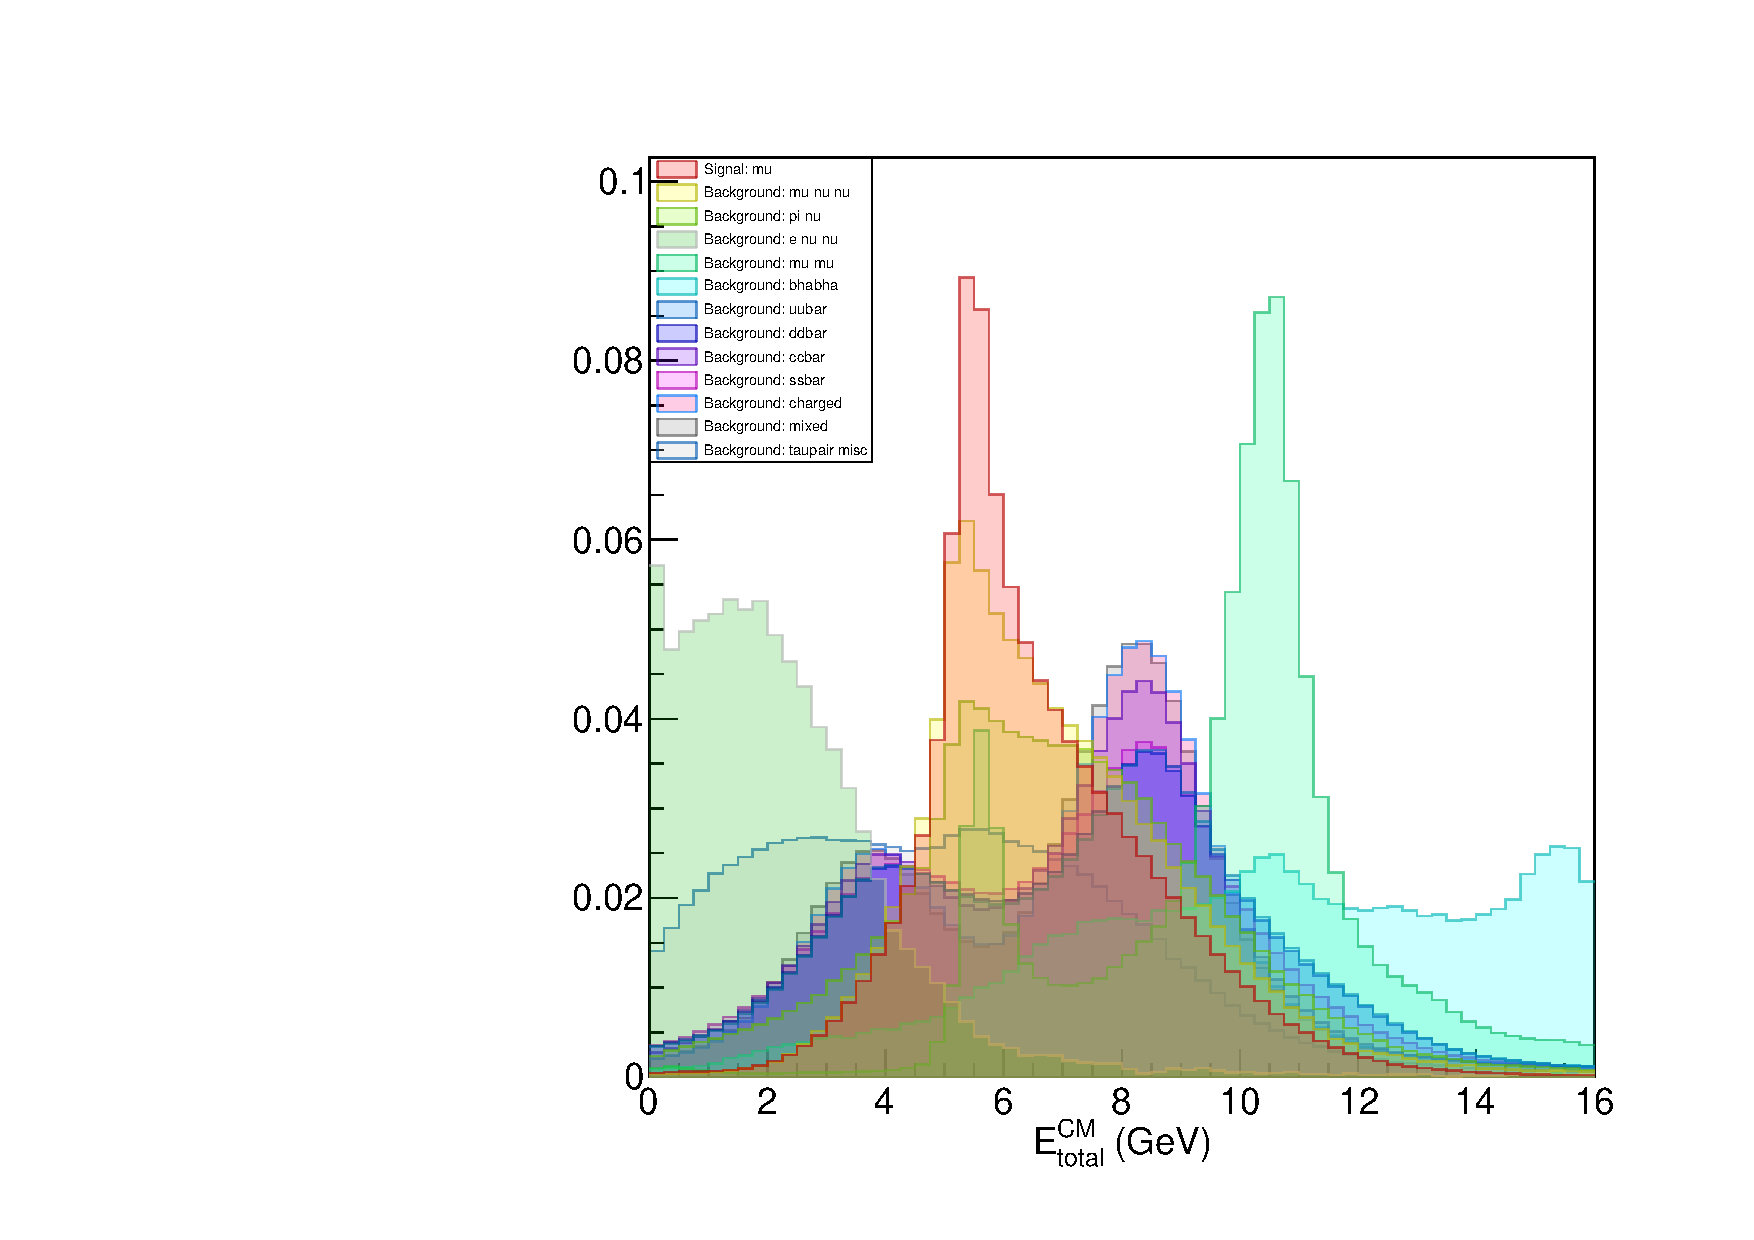
\includegraphics[width=\textwidth]{images/test.pdf}
            \caption[Network2]%
            {{\small Network 1}}    
            \label{fig:mean and std of net14}
        \end{subfigure}
        \hfill
        \begin{subfigure}[b]{0.475\textwidth}  
            \centering 
            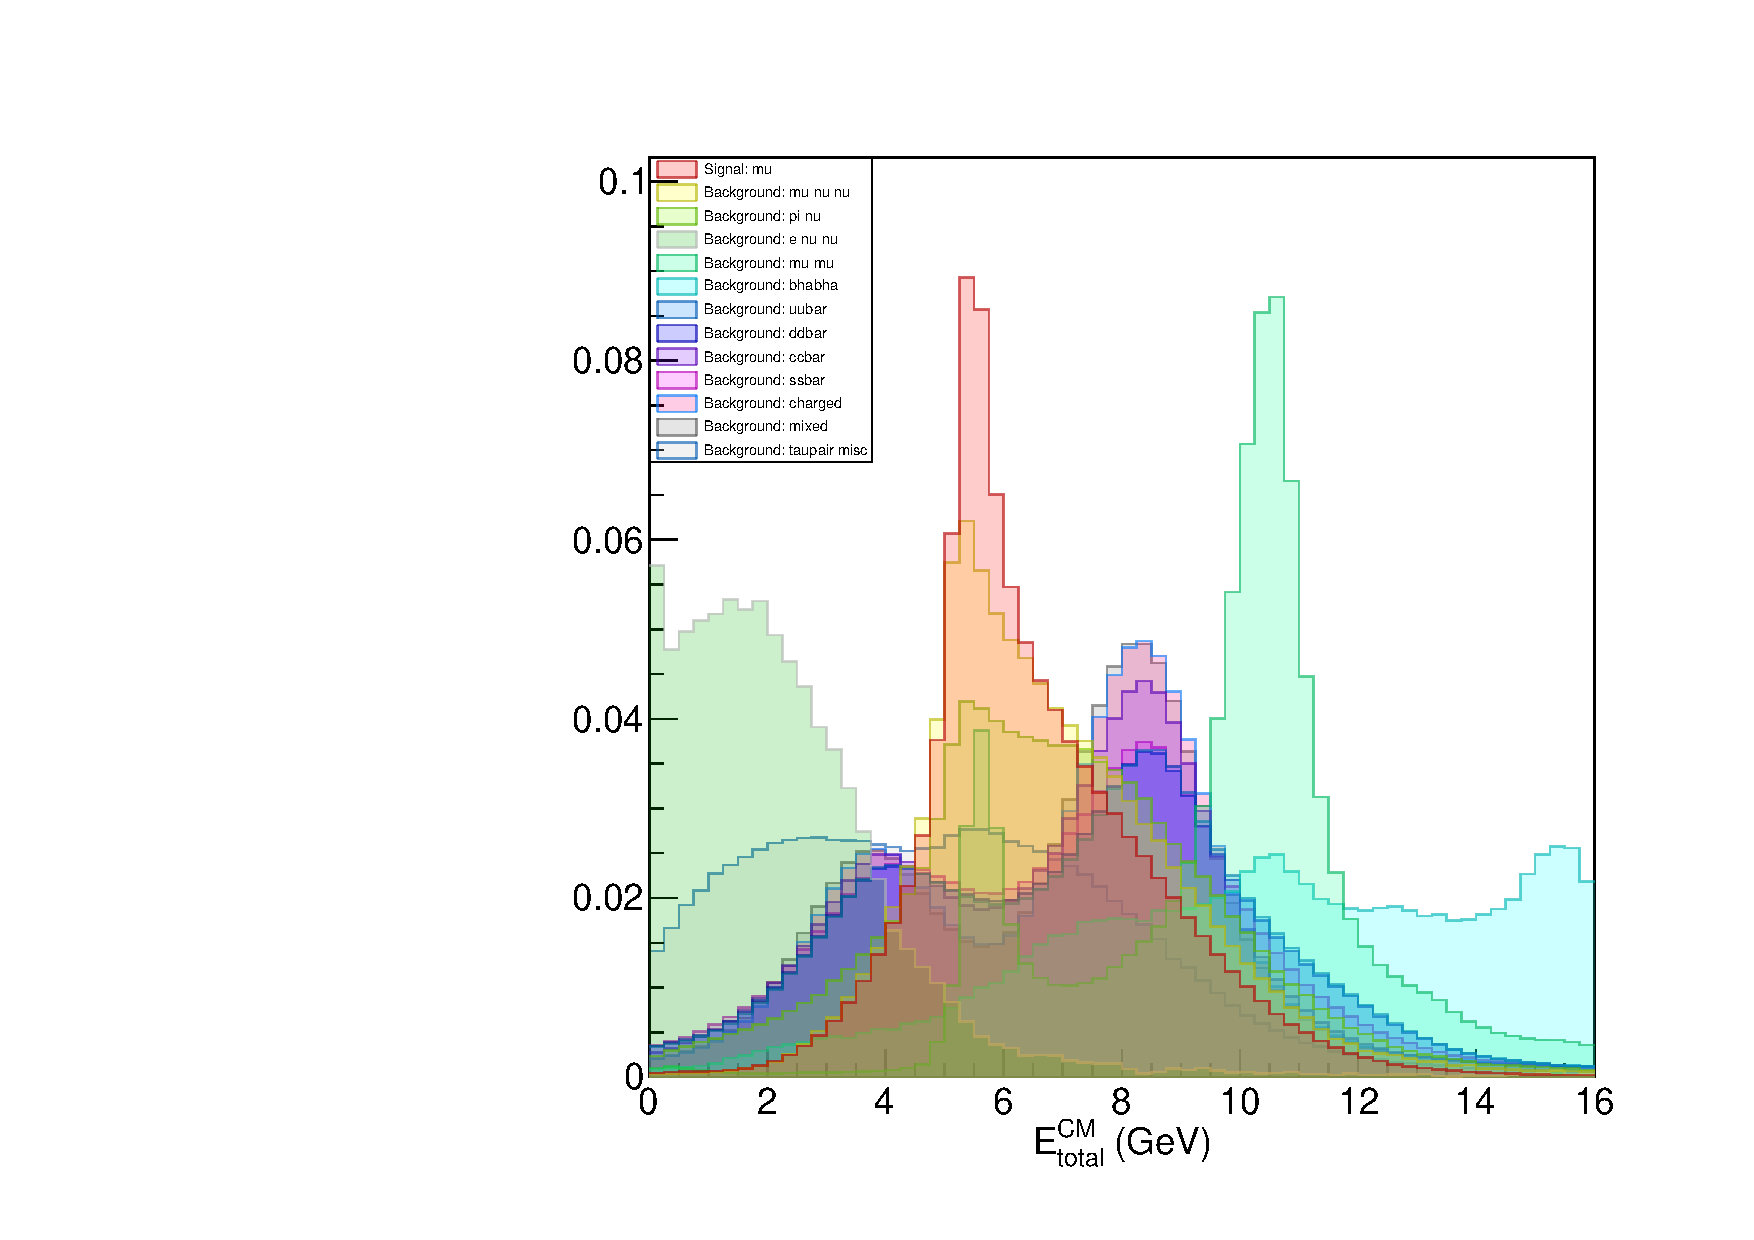
\includegraphics[width=\textwidth]{images/test.pdf}
            \caption[]%
            {{\small Network 2}}    
            \label{fig:mean and std of net24}
        \end{subfigure}
        \vskip\baselineskip
        \begin{subfigure}[b]{0.475\textwidth}   
            \centering 
            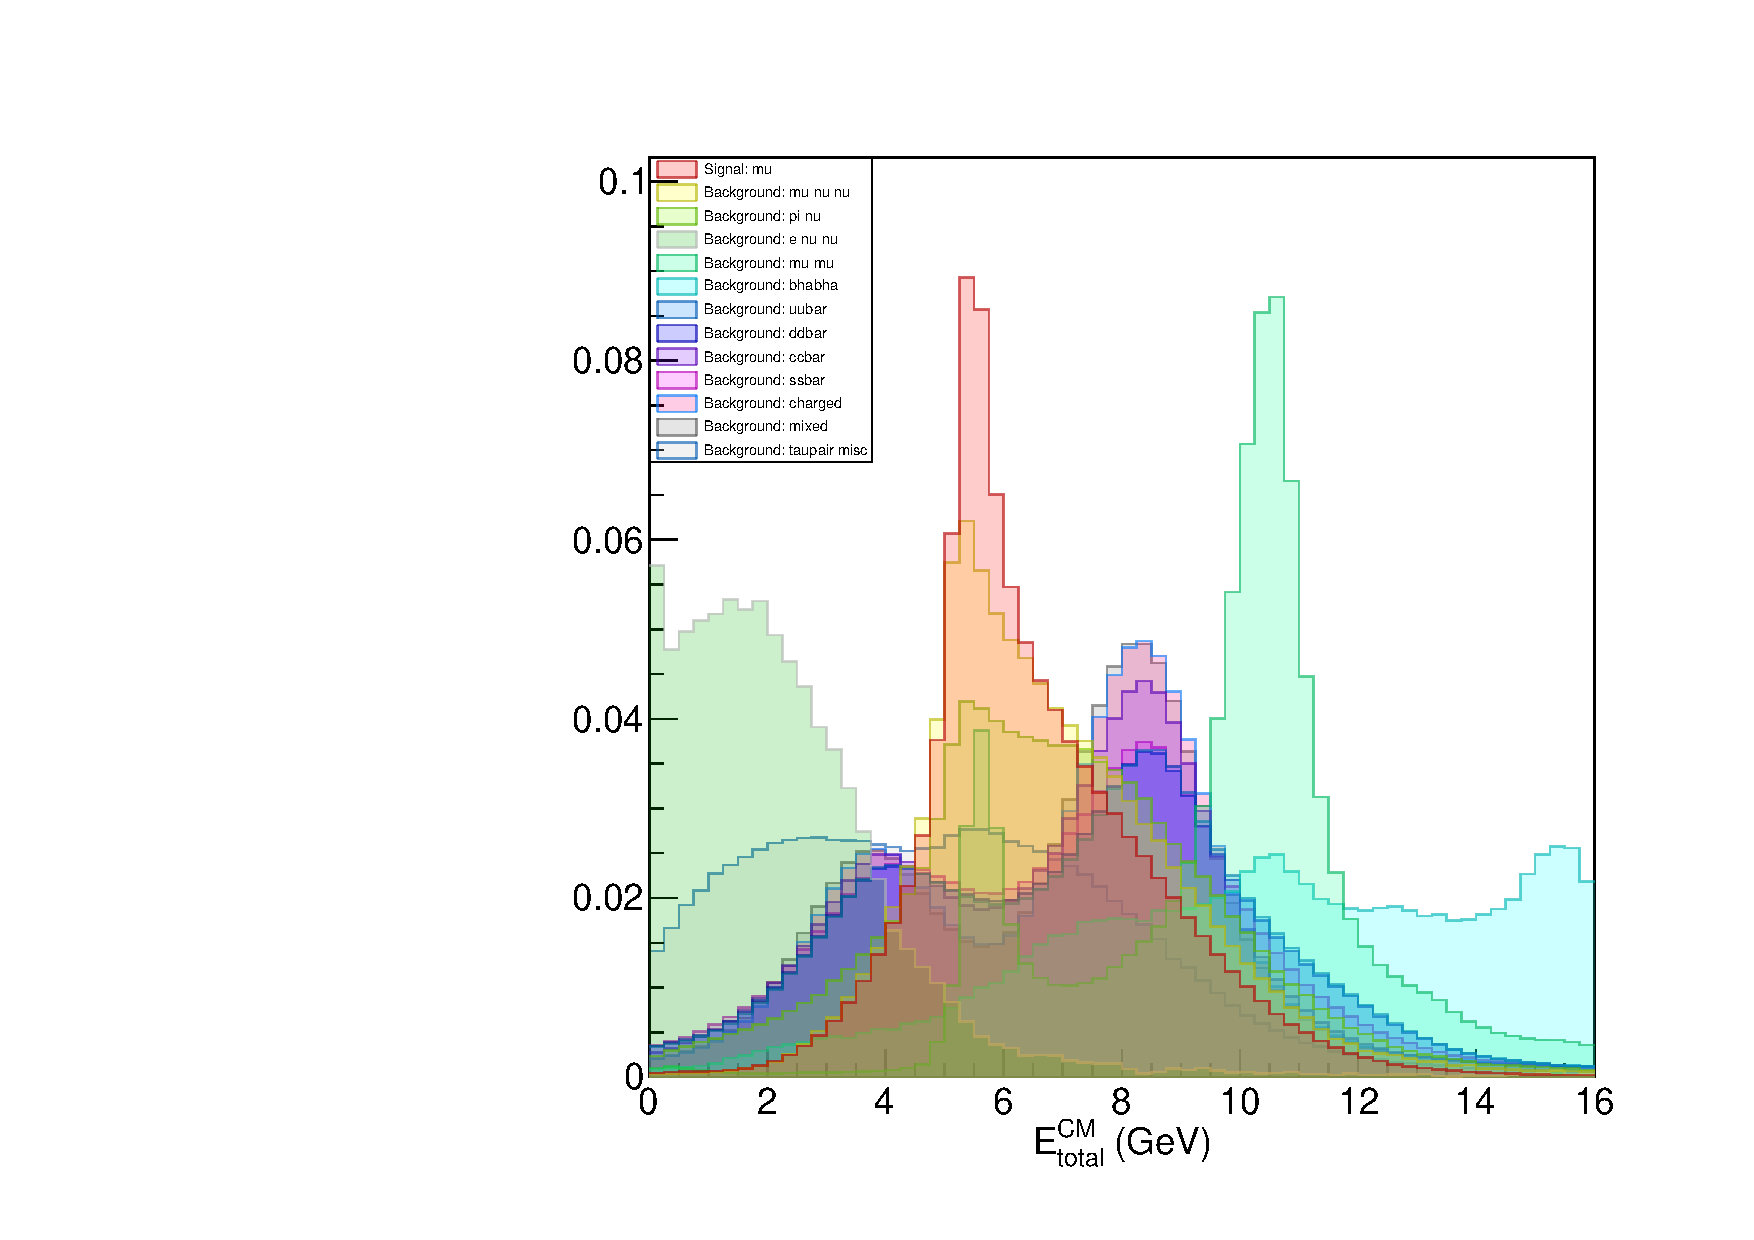
\includegraphics[width=\textwidth]{images/test.pdf}
            \caption[]%
            {{\small Network 3}}    
            \label{fig:mean and std of net34}
        \end{subfigure}
        \quad
        \begin{subfigure}[b]{0.475\textwidth}   
            \centering 
            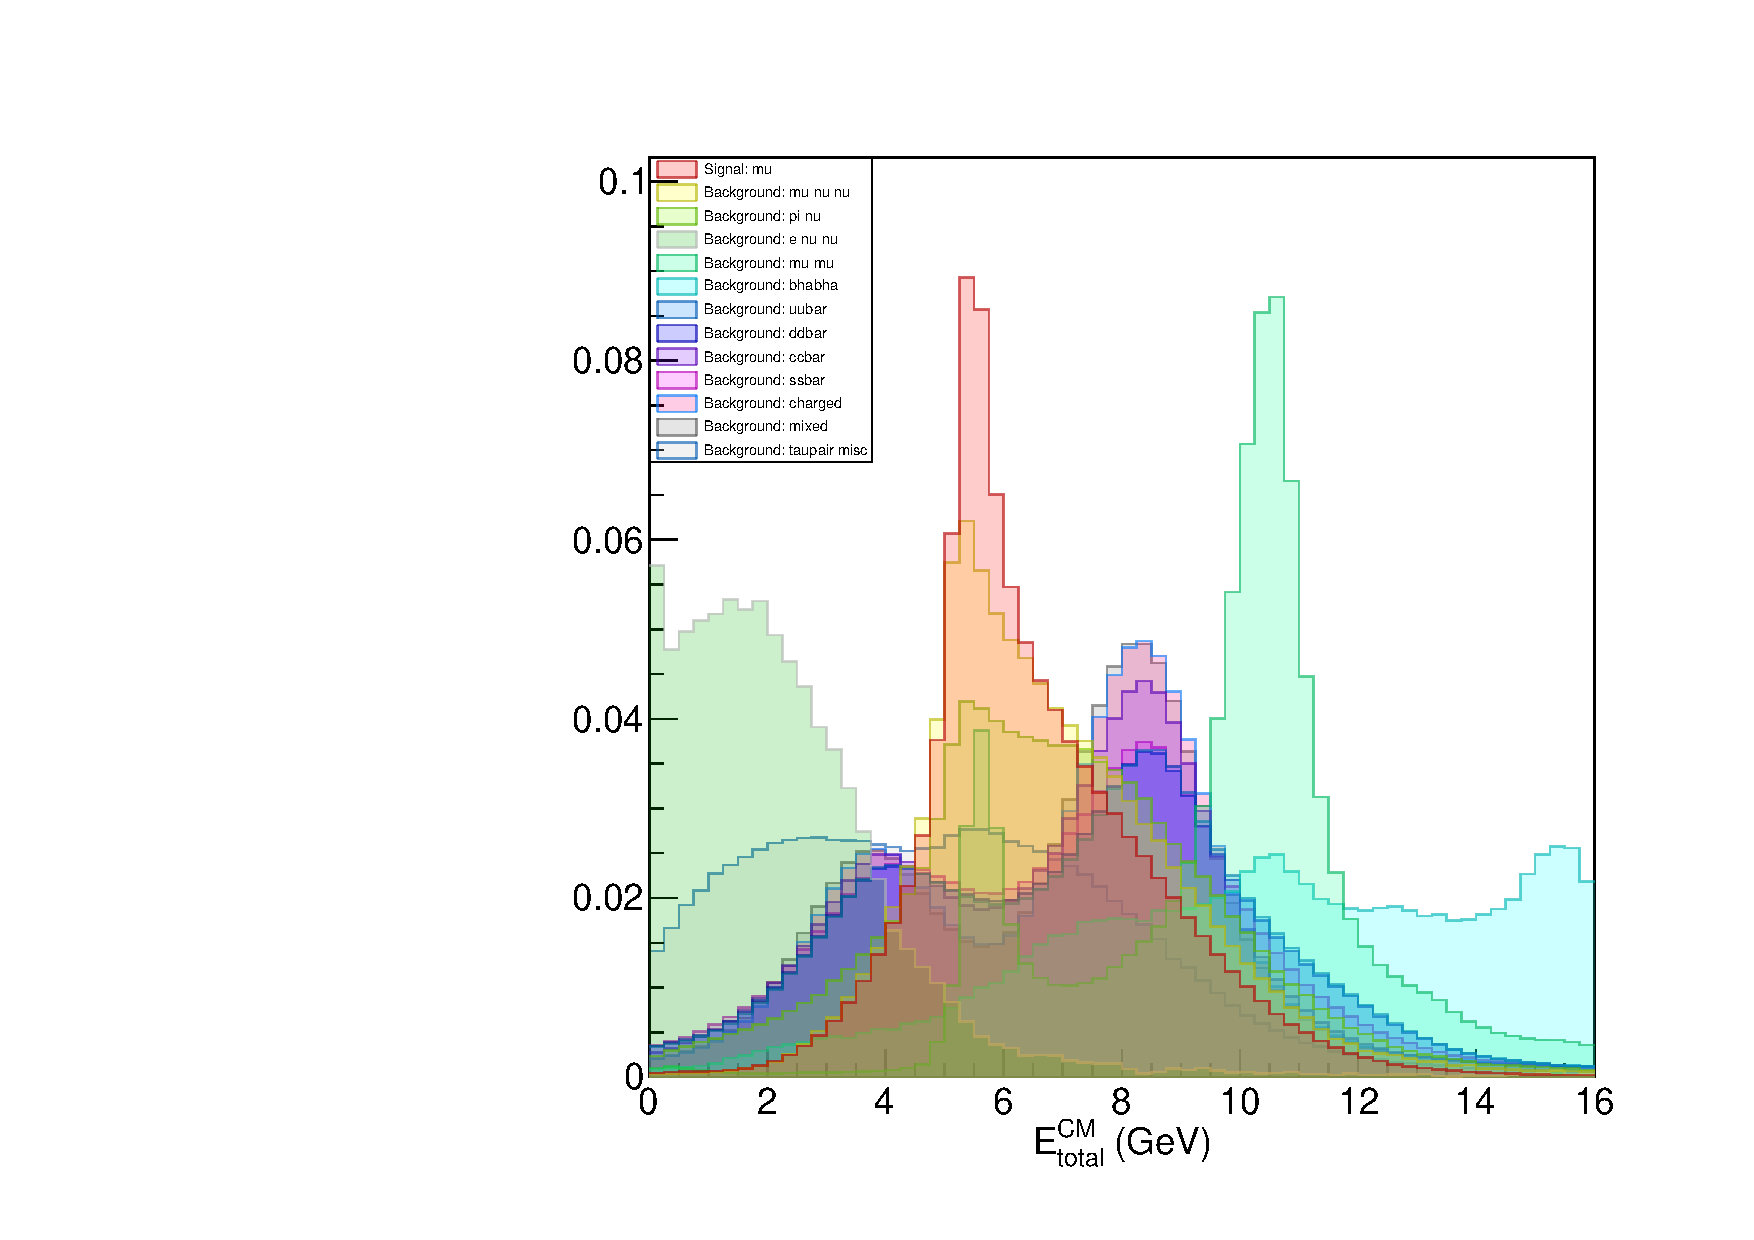
\includegraphics[width=\textwidth]{images/test.pdf}
            \caption[]%
            {{\small Network 4}}    
            \label{fig:mean and std of net44}
        \end{subfigure}
        \label{fig:mean and std of nets}
                \vskip\baselineskip
                \begin{subfigure}[b]{0.475\textwidth}   
            \centering 
            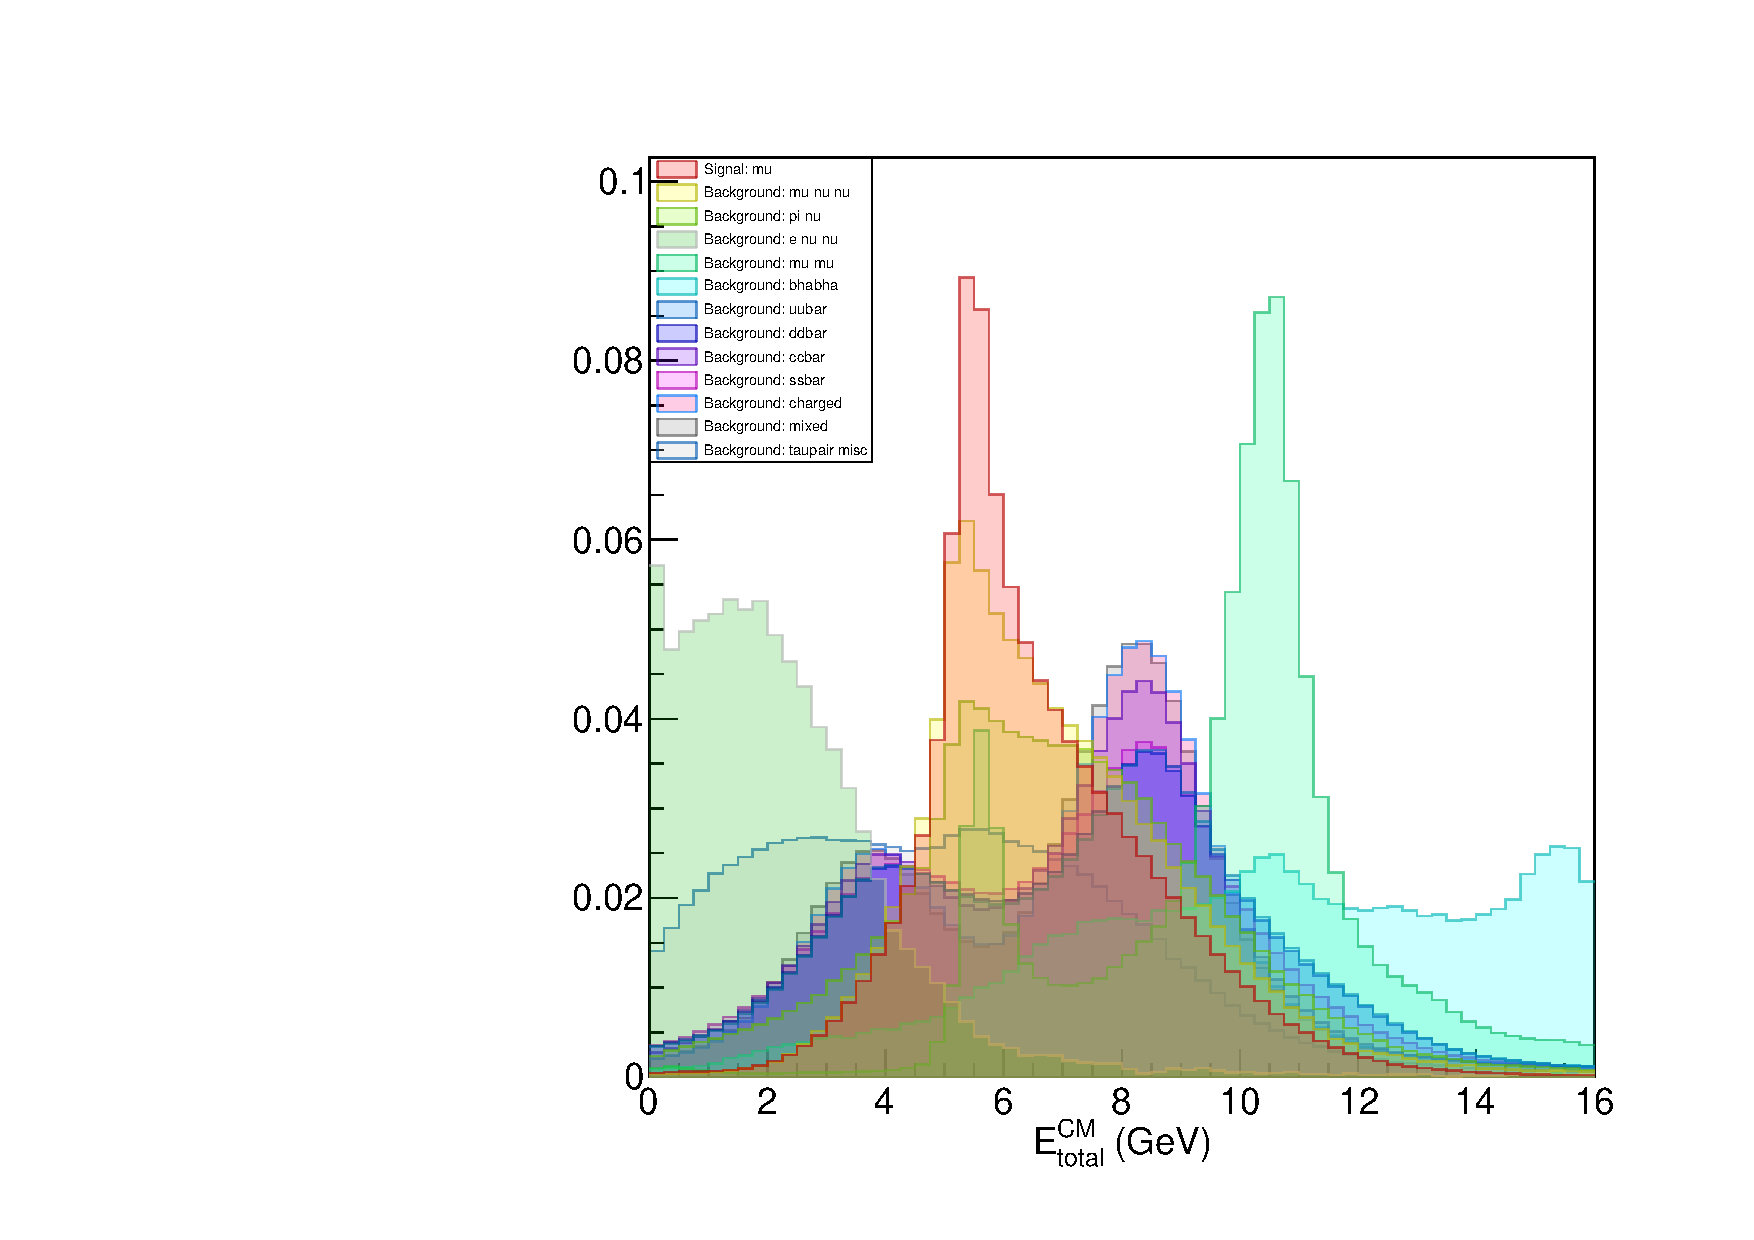
\includegraphics[width=\textwidth]{images/test.pdf}
            \caption[]%
            {{\small Network 3}}    
            \label{fig:mean and std of net34}
        \end{subfigure}
                \caption[ The average and standard deviation of critical parameters ]
        {\small The average and standard deviation of critical parameters: Region R4} 
    \end{figure}


\begin{table}[h]
\centering
\begin{tabular}{lrrc}
\textbf{MC type}         & \textbf{events in (scaled)} & \textbf{events out} & $\mathbf{\epsilon_{\text{ps}}}$ \\ \hline 
\rowcolor[HTML]{EFEFEF} 
$\tau\to\mu\gamma$       & \num{140}        & \num{135}      & $\SI{96.32}{\percent}$                   \\
$\tau\to\mu\nu\nu$      & \num{678130}         & \num{631235}          & $\SI{93.08}{\percent}$           \\
$\tau\to\pi\nu$         & \num{1076758}       & \num{822028}          & $\SI{76.34}{\percent}$            \\
$\tau\to e\nu\nu$       & \num{109810}        & \num{70675}         & $\SI{64.36}{\percent}$      \\
$\tau\to\text{generic}$  & \num{2304225}       & \num{636954}          & $\SI{27.64}{\percent}$         \\
$e^+ e^- \to \mu^+ \mu^- (\gamma)$   & \num{39857811}    & \num{21938180}     & $\SI{55.04}{\percent}$   \\
$e^+ e^- \to e^+ e^- (\gamma)$      & \num{7111247601}      & \num{1457005758}       & $\SI{20.49}{\percent}$     \\
$e^+ e^- \to u \bar{u}$       & \num{66447114}           & \num{29767142}  & $\SI{44.80}{\percent}$ \\
$e^+ e^- \to d \bar{d}$        & \num{16384978}       & \num{7307320}      & $\SI{44.60}{\percent}$       \\
$e^+ e^- \to c \bar{c}$        & \num{6017200}       & \num{23401910}           & $\SI{38.99}{\percent}$          \\
$e^+ e^- \to s \bar{s}$       & \num{14579500}     & \num{6299797}            & $\SI{43.21}{\percent}$         \\
$e^+ e^- \to B^+ B^-$     & \num{56664730}       & \num{22083348}           & $\SI{38.97}{\percent}$          \\
$e^+ e^- \to B^0 \bar{B}^0$       & \num{60329511}           & \num{23372366}        & $\SI{61.26}{\percent}$              
\end{tabular}
\caption{Preselection efficiency}
\label{my-label}
\end{table}


\section{Electron mode}

Separate preselection criteria was chosen for the electron mode. These criteria do not differ much, as expected, however due to the prevalence of bremsstrahlung in the electron mode the energy variables differ greatly. Due to this we set an upper limit on $E^{\text{CM}}_{\text{sum}}$ rather than a lower limit as for the muon mode.

\begin{figure}[h]
\centering
\begin{minipage}{.5\textwidth}
  \centering
  \includegraphics[width=\linewidth]{images/stack/stack_cut6_totalCM_E.pdf}
  \captionof{figure}{A figure}
  \label{fig:test1}
\end{minipage}%
\begin{minipage}{.5\textwidth}
  \centering
  \includegraphics[width=\linewidth]{images/stack/stack_cut6_totalCM_E.pdf}
  \captionof{figure}{Another figure}
  \label{fig:test2}
\end{minipage}
\end{figure}

\begin{table}[h]
\centering
\begin{tabular}{llll}
\textbf{symbolic} & \textbf{description} & \textbf{lower} & \textbf{upper} \\ \hline
$p_{\text{tag}}^{\text{CM}}$  & CM momentum of tag track & --- & $\SI{5}{GeV}$ \\
$\cos\theta_{\text{signal}}$ & Cosine of polar angle of signal track & $-0.975$ & --- \\
$E_{\text{total}}^{\text{CM}}$ & Center-of-mass energy of total system  & --- & $\SI{14}{GeV}$ \\
$\lvert\text{thrust}\rvert$ & Magnitude of signal thrust vector* & 0.92 & --- \\
$E_{\text{sum}}^{\text{CM}}$ & Center-of-mass energy of photons and tracks & $\SI{4.5}{GeV}$ & ---
\end{tabular}
\caption{Preselection cuts (electron mode)}
\label{my-label}
\end{table}

  \begin{figure}
        \centering
        \begin{subfigure}[b]{0.475\textwidth}
            \centering
            \includegraphics[width=\textwidth]{images/test.pdf}
            \caption[Network2]%
            {{\small Network 1}}    
            \label{fig:mean and std of net14}
        \end{subfigure}
        \hfill
        \begin{subfigure}[b]{0.475\textwidth}  
            \centering 
            \includegraphics[width=\textwidth]{images/test.pdf}
            \caption[]%
            {{\small Network 2}}    
            \label{fig:mean and std of net24}
        \end{subfigure}
        \vskip\baselineskip
        \begin{subfigure}[b]{0.475\textwidth}   
            \centering 
            \includegraphics[width=\textwidth]{images/test.pdf}
            \caption[]%
            {{\small Network 3}}    
            \label{fig:mean and std of net34}
        \end{subfigure}
        \quad
        \begin{subfigure}[b]{0.475\textwidth}   
            \centering 
            \includegraphics[width=\textwidth]{images/test.pdf}
            \caption[]%
            {{\small Network 4}}    
            \label{fig:mean and std of net44}
        \end{subfigure}
        \label{fig:mean and std of nets}
                \vskip\baselineskip
                \begin{subfigure}[b]{0.475\textwidth}   
            \centering 
            \includegraphics[width=\textwidth]{images/test.pdf}
            \caption[]%
            {{\small Network 3}}    
            \label{fig:mean and std of net34}
        \end{subfigure}
                \caption[ The average and standard deviation of critical parameters ]
        {\small The average and standard deviation of critical parameters: Region R4} 
        \end{figure}


\begin{table}[h]
\centering
\begin{tabular}{lrrc}
\textbf{Event type}         & \textbf{events in (scaled)} & \textbf{events out} & $\mathbf{\epsilon_{\text{ps}}}$ \\ \hline 
\rowcolor[HTML]{EFEFEF} 
$\tau\to e\gamma$       & \num{140}        & \num{135}      & $\SI{96.32}{\percent}$                   \\
$\tau\to\mu\nu\nu$      & \num{678130}         & \num{631235}          & $\SI{93.08}{\percent}$           \\
$\tau\to\pi\nu$         & \num{1076758}       & \num{822028}          & $\SI{76.34}{\percent}$            \\
$\tau\to e\nu\nu$       & \num{109810}        & \num{70675}         & $\SI{64.36}{\percent}$      \\
$\tau\to\text{generic}$  & \num{2304225}       & \num{636954}          & $\SI{27.64}{\percent}$         \\
$e^+ e^- \to \mu^+ \mu^- (\gamma)$   & \num{39857811}    & \num{21938180}     & $\SI{55.04}{\percent}$   \\
$e^+ e^- \to e^+ e^- (\gamma)$      & \num{7111247601}      & \num{1457005758}       & $\SI{20.49}{\percent}$     \\
$e^+ e^- \to u \bar{u}$       & \num{66447114}           & \num{29767142}  & $\SI{44.80}{\percent}$ \\
$e^+ e^- \to d \bar{d}$        & \num{16384978}       & \num{7307320}      & $\SI{44.60}{\percent}$       \\
$e^+ e^- \to c \bar{c}$        & \num{6017200}       & \num{23401910}           & $\SI{38.99}{\percent}$          \\
$e^+ e^- \to s \bar{s}$       & \num{14579500}     & \num{6299797}            & $\SI{43.21}{\percent}$         \\
$e^+ e^- \to B^+ B^-$     & \num{56664730}       & \num{22083348}           & $\SI{38.97}{\percent}$          \\
$e^+ e^- \to B^0 \bar{B}^0$       & \num{60329511}           & \num{23372366}        & $\SI{61.26}{\percent}$              
\end{tabular}
\caption{Preselection efficiency}
\label{my-label}
\end{table}

\pagebreak

%-------------------------------------------------------------------

\begin{comment}
\chapter{Correlation}

The final signal region in which events will be selected from lies in $\Delta E$ vs. $M_{\text{inv}}$ space. To avoid biasing event selection, only loose cuts are applied to these variables throughout. We also investigate the correlation between these signal variables and other variables which we may cut over, to avoid introducing bias through these correlations. 

???

\pagebreak
\end{comment}

%-------------------------------------------------------------------

\chapter{Signal optimisation}

(DISCUSS $S/\sqrt{S+B}$, what it is and why we optimise it.)

There are many reasonable ways to quantify signal optimisation compared to background in a particle physics analysis. For this analysis, we have chosen the measure of signal optimisation $S/\sqrt{S+B}$. $S$ is the expected number of signal events remaining after event selection has been performed; note that we scale for our signal events dependent on their associated LFV branching fractions, which are currently experimental upper bounds. Hence the measure $S/\sqrt{S+B}$ will vary for different branching fraction hypotheses. 
Similarly $B$ is the expected number of background events remaining after event selection; specifically this is the sum of all events remaining across all background MC used in analysis. Since not all possible background processes have been included we would expect the empirical value of $B$ to be higher; this is mostly unimportant for our analysis since we need only compare changes in $S/\sqrt{S+B}$ between different selection criteria, not to know the absolute value.
\\
To maximise $S/\sqrt{S+B}$, the number of background events must be reduced while not removing too many sgnal events. This is especially important given the low branching fraction of our signal - taking the experimental upper limit of the $\tau\to\mu\gamma$ ($\tau\to e\gamma$) branching fraction, we expect only 135 (XXX) signal events, after reconstruction and preselection, in a $\SI{1000}{fb^-1}$ dataset, compared to over \num{1500000000} (1.5 billion) background events in the same luminosity. The actual number of signal events is very likely lower, due to double-counting in reconstruction (REPHRASE. Also, something to say about lower branching fraction?).
\\
Forty selection criteria were used in selecting for $\tau\to\mu\gamma$ events. Variables chosen for selection originally came from the previous search for $\tau\to\ell\gamma$ at Belle (REF); more were added as the analysis progressed to achieve better greater signal separation. Some of these variables were not included in the final analysis. Notable were those related to missing momentum and mass, excluded due to poor reconstruction resulting in poor event separation. Others such as tag-track transverse momentum and signal-track momentum were not included due to significant overlap of background exclusion with other variables (most obviously center-of-mass tag track momentum and center-of-mass signal-track momentum) causing selection on these measureables to have little to no impact on signal optimisation.
\\
The thresholds were chosen via a manuallly iterative process, continually improving the ratio $S/\sqrt{S+B}$ by adding or refining criteria. Initial criteria were informed by a combination of automatic iteration over a range of threshold values for around 20 variables, and by visual inspection.

The accomplish the former, selection was repeatedly performed over all MC with only a single criteria applied. The lower or upper threshold of this criteria was modified by a small increment each time. The resulting value of $S/\sqrt{S+B}$ was then plotted against the selection threshold; this plot is called a \emph{figure-of-merit} plot. An obvious peak, as in Figure XXXX, indicates a beneficial (??) value for selection. For many variables, no peak was apparent and so no initial threshold could be chosen through this method.

\begin{figure}[h]
\centering
\includegraphics[width=0.7\linewidth]{images/fom-test.pdf}
\caption{Figure-of-merit plot for $p_{\text{signal}}^{\text{CM}}$}
\label{}
\end{figure}

Initial visual inspection was performed by finding obvious separation between signal and many background variables. This was informed by knowledge of event topologies (Section XXXX), as well as some figure-of-merit plots as described above. Figures XXXX and XXXXX are examples of good and poor selection variables. In Figure XXXX, large background peaks occuring at less than $\SI{1}{GeV/c}$ and greater than $\SI{4.3}{Gev}$ lead to great separation from signal, which does not peak anywhere in those regions. Figure XXXX offers less than optimal threshold positions, as there is no apparent way to remove any amount of background without also removing a large amount of signal; note that this variable was not included during event selection. 

\begin{figure}[h]
\centering
\begin{minipage}{.5\textwidth}
  \centering
  \includegraphics[width=\linewidth]{images/tauMG-muCM_P.pdf}
  \captionof{figure}{muCM P}
  \label{fig:test1}
\end{minipage}%
\begin{minipage}{.5\textwidth}
  \centering
  \includegraphics[width=\linewidth]{images/tauMG-missingCosTheta.pdf}
  \captionof{figure}{missingCosTheta}
  \label{fig:test2}
\end{minipage}
\end{figure}

\section{Muon mode}

Figure XXXX shows the number of signal and background events remaining after selection has been applied. Specific discussion and justification of selection criteria is given below.

\begin{table}[h]
\centering
\begin{tabular}{lrr}
\textbf{Event process}         & \textbf{events in} & \textbf{events out} \\ \hline 
\rowcolor[HTML]{EFEFEF} 
$\tau\to\mu\gamma$       & \num{135 \pm 1}        & 6                             \\
$\tau\to\mu\nu\nu$      & \num{631235}             & 163                    \\
$\tau\to\pi\nu$         & \num{822028}                & 40                                     \\
$\tau\to e\nu\nu$       & \num   {70675}              & 0                                  \\
$\tau\to\text{generic}$  & \num{636954}           & 0                                   \\
$e^+ e^- \to \mu^+ \mu^- (\gamma)$       & \num{21938180}        & 15             \\
$e^+ e^- \to e^+ e^- (\gamma)$      & \num{1457005758}      & 0                               \\
$e^+ e^- \to u \bar{u}$       & \num{29767142}           & 9                                 \\
$e^+ e^- \to d \bar{d}$        & \num{7307320}           & 3                                \\
$e^+ e^- \to c \bar{c}$        & \num{23401910}           & 0                            \\
$e^+ e^- \to s \bar{s}$       & \num{6299797}           & 3                                       \\
$e^+ e^- \to B^+ B^-$     & \num{22083348}           & 0                            \\
$e^+ e^- \to B^0 \bar{B}^0$       & \num{23372366}           & 0                           
\end{tabular}
\caption{Events remaining after selection (electron mode)}
\label{my-label}
\end{table}

\subsection{Energy-momentum}

{\large I need some way to say this without saying ``we require'' repeatedly. Could borrow from Hayasaka-san}

We require $p^{\text{CM}}_{\mu}$ greater than $\SI{1}{GeV/c}$ and less than $\SI{4.3}{GeV/c}$, to remove low-momentum tracks from continuum events and to remove high-momentum tracks from leptonic processes without high-energy final state photons, that is, generic tau-pair processes, mu-pair processes, and bhabha. Muon transerve momentum $p^{\text{t}}_{\mu}$ is required to be greater than $\SI{0.1}{GeV/c}$; tracks with a lesser transverse momentum could not reach the CDC sub-detector component so we do not select these events. Low-energy tracks from continuum events often do not satisfy this criteria, however most low-energy tracks are excluded through selection on $p^{\text{CM}}_{\mu}$. To suppress $\mu^+\mu^-$ and Bhabha backgrounds we require center-of-mass momentum of the tag track $p^{\text{CM}}_{\text{tag track}}$ less than $\SI{2.5}{GeV}$. Through conservation of momentum we expect the signal and tag tracks of the processes $e^+ e^-\to\ell^+ \ell^- (\gamma)$ we to have momentum peaks around $\SI{5}{GeV}$, which are excluded by this selection. Since most background processes reconstruct the signal photon from low-energy photons, we require the energy of the signal photon $E_{\gamma}$ to be $\SI{0.8}{GeV}$. This selection criteria is effective in removing background events across different processes. Total energy in the center-of-mass frame $E^{\text{CM}}_{\text{total}}$ is required to be less than $\SI{12}{GeV}$ to suppress $\mu^+\mu^-$ events.

NOTE: variables I didn't use but could have used = $p^{\text{t}}_{\text{tag track}}$, $p_{\mu}$, $E^{\text{CM}}_{\text{sum}}$


\subsection{Topological relations}

We require $\cos\theta_{\mu}$ in the range \num{-0.8} to \num{0.9}; \num{-0.8} < $\cos\theta_{\gamma}$ < \num{0.85}; \num{1} < $\theta^{\text{CM}}_{\text{signal $\tau$}}$ < \num{2.2}; -0.8 < $\cos\theta_{\text{H}}$ < 0.8.

DISCUSS, ELABORATE, ETC.

\subsection{PID likelihoods}

Signal-side tracks are identified as muons by requiring $\mathcal{L}_{\mu} > 0.8$. To reduce the effect of double-counting, mostly for signal events, we require $\mathcal{L}_{K} < 0.08$ and $\mathcal{L}_{e} < 0.005$. Due to how events are reconstructed in \texttt{basf2} we also require $\mathcal{L}_{\pi} > 0.8$ (WHY IS THIS??). On the tag-side, we require $\mathcal{L}_{\mu} < 0.85$ to identify the tag-track as not a muon.

SOMETHING ABOUT $\mathcal{L}_{\mu}$ being not perfect? Very rough on the tag-side.


\subsection{Background suppression using event shape}

\hrule

We start with a note on naming of ``continuum suppression'' variables. Physics analyses at B-factories such as Belle and Belle II often involve decays of $B$ mesons (a hadron composed of a quark and anti-quark) generated via the process $e^+ e^- \to \Upsilon(4S)\to B \bar{B}$. $\upsilon(4S)$ is a meson generated in $e^+ e^-$ collisions at the a combined center-of-mass beam energy of $\SI{10.58}{GeV}$ (known as the $\Upsilon(4S)$ resonance) which decays to $B\bar{B}$ in \num{96}{\percent} of all decays. At this resonance many other $e^+ e^-$ decay processes occur, so that the event rate is dominated by non-$B$ background processes. The dominant source of background is from $e^+ e^- \to q\bar{q}$ events, known as continuum events. To effectively suppress these events a suite of variables which provide good discrimination between $B$ events and continuum events have been developed for use at $B$-factories. In a $\tau$ decay analysis, these variables do not suppress continuum background as strongly as for $B$ decays. However they are still useful in removing some continuum as well as other backgrounds as discussed later, so with somewhat of a historical basis we shall refer to these variables as continuum suppression variables. Continuum suppression variables included in this analysis are signal and rest-of-event thrust, cosine of the angle between signal and rest-of-event thrust axes,  CLEO cones, Super Fox-Wolfram moments, and the reduced Fox-Wolfram moment (the ratio of the second to the zeroth Fox-Wolfram moments).

(\textbf{note: now that I've renamed this section from ``Continuum suppression'', not sure I need this. Nor if I needed it in the first place. Some possibily still useful stuff though?}).
\hrule

The thrust axis for a collection of $N$ particles with momenta $\mathbf{p}_{i}$ ($i = 1,\ldots, N$) is defined as the unit vector along with the total projection of these momenta is maximised. The thrust scalar, or thrust, is defined as
\begin{equation}
T = \frac{\sum^N_{i=1}\lvert\mathbf{T}\cdot\mathbf{p}_i\rvert}{\sum^N_{i=i}\lvert\mathbf{p}_i\rvert}.
\end{equation}
Signal thrust and rest-of-event thrust variables are used for selection. The signal thrust axis is constructed from all particles used to reconstruct the signal-side $\tau$; for our signal mode these are the signal muon and signal photon. On average these particles have similar momentum and a small opening between them, so that signal thrust has a clear peak around \num{0.942}. We consider the signal thrust axis for the other dominant leptonic processes. For most events the signal-side is reconstructed from a high-energy charged track and a low-energy photon generated from bremsstrahlung, beam background or similar (radiative mu-pair or Bhabha events can generate higher energy final-state photons). Regardless of opening angle, the difference in momentum between signal track and signal photon leads to signal thrust for this event peaking around \num{1}. A requirement for signal thrust to be in the range \num{0.936} to \num{0.944} to suppress leptonic backgrounds as shown in Figure XXXX. 

\begin{figure}[h]
\centering
\begin{minipage}{.5\textwidth}
  \centering
  \includegraphics[width=\linewidth]{images/tauMG-thrustSignal.pdf}
  \captionof{figure}{Signal thrust}
  \label{fig:test1}
\end{minipage}%
\begin{minipage}{.5\textwidth}
  \centering
  \includegraphics[width=\linewidth]{images/tauMG-thrustRoe.pdf}
  \captionof{figure}{Rest-of-event thrust}
  \label{fig:test2}
\end{minipage}
\end{figure}


We construct another thrust axis is also built using rest-of-event (ROE) data. ROE comprises all tracks and clusters not associated with the signal-side reconstruction, and so ROE thrust is influenced by tag-side events. Hadronic processes such as $B\bar{B}$ events and continuum have on average a lower rest-of-event thrust than leptonic processes due to the number of tracks and photons produced due to interactions with the detector. The magnitude of this ROE thrust vector is required to be in the range from \num{0.85} and \num{0.98}. As shown in Figure XXXX, events produce very clean Gaussian-like distributions with little trailing tail. As such, while this selection removes a non-negligible amount of signal, it suppresses continuum events very strongly and almost completely excludes $B\bar{B}$ events. Event selection is also performed using the angle between thrust axes. We require the cosine of the angle between the signal thrust vector and rest-of-event thrust vector to be greater than \num{0.7}.


Several continuum suppression variables were chosen by inspection after many more obvious criteria had been applied. These are CLEO cones, Super Fox-Wolfram moments, and the reduced Fox-Wolfram moment (the ratio of the second to the zeroth Fox-Wolfram moments).

Inherent differences in event shape can be used to suppress backgrounds. Some useful disciminant variables are the CLEO cones, named as such due to being introduced in a 1995 paper by the CLEO collaboration (REF). To calculate these variables, the space around the signal thrust axis is divided into cones at nine polar angle intervals of $10^{\deg}$ each, with the $i^{th}$ interval covering angles from $(i-1)\times 10^{\deg}$ to $i\times 10^{\deg}$ from the thrust axis (see Figure XXXX). Forward and backward intervals are combined. CLEO cone variables cc$i$ are defined as the lab-frame momentum flow of the $i^{th}$ cone; momentum flow in each cone is calculated as the scalar sum of all tracks and clusters in that cone.

\begin{figure}[h]
\centering
\includegraphics[width=0.5\linewidth]{images/cleo-cone.png}
\caption{Illustration of cleo cones.}
\label{}
\end{figure}

Requirements on CLEO cones are given in Table XXXX.

\begin{table}[h]
\centering
\begin{tabular}{lll}
\textbf{CLEO cone} & \multicolumn{1}{c}{\textbf{lower}} & \multicolumn{1}{c}{\textbf{upper}} \\ \hline
cc1 & -- & \num{5} \\
cc2 & \num{2.4} & -- \\
cc3 & -- & -- \\
cc4 & -- & \num{1.7} \\
cc5 & -- & \num{0.9} \\
cc6 & -- & \num{0.7} \\
cc7 & -- & \num{0.5} \\
cc8 & -- & -- \\
cc9 & -- & \num{0.4}
\end{tabular}
\caption{Cleo cone selection criteria}
\label{my-label}
\end{table}

Fox-Wolfram moments (FWM) are event shape variables which describe energy flow from high-energy particle collision events, introduced to describe $e^+ e^-$ annihilation event shapes. Variables $h^{so}_i$ ($i=2,4$) and $h^{oo}_j$ are the normalised FWM, defined as
\begin{equation}
h_l^k = \frac{\sum_{m,n}\lvert\vec{p_m}\rvert\lvert\vec{p_n}\rvert P_l(\cos\theta_{mn})}
{\sum_{m,n}\lvert\vec{p_m}\rvert\lvert\vec{p_n}\rvert},
\end{equation}
where $\vec{p_m}$ and $\vec{p_n}$ are the momenta of particles $m$ and $n$ and $P_l(\cos\theta_{mn})$ is the $l$-th other Legendre polynomial of cosine of the angle $\theta_{mn}$ between $\vec{p_m}$ and $\vec{p_n}$. We categorise the type of FWM with $k=so,oo$. For $h^{so}_i$, $m$ is from signal particles and $n$ is from ROE; for $h^{oo}_{j}$ both $m$ and $n$ are from ROE.

\begin{table}[h]
\centering
\begin{tabular}{lll}
\textbf{FWM} & \multicolumn{1}{c}{\textbf{lower}} & \multicolumn{1}{c}{\textbf{upper}} \\ \hline
Hso(0,0) & \num{0.05} & \num{1} \\
Hso(0,1) & \num{-0.05} & \num{0.3} \\
Hso(0,2) & -- & \num{0.48} \\
Hso(0,3) & \num{-0.1} & \num{0.25} \\
Hso(2,0) & \num{-0.1} & \num{1} \\
Roo(1) & \num{-0.018} & \num{0.08} \\
Roo(3) & \num{-0.01} & \num{0.007}
\end{tabular}
\caption{Super Fox-Wolfram moment selection criteria}
\label{my-label}
\end{table}
\textbf{Note: not entirely sure what Hso(0,0) etc. means}

A final continuum suppression requirement is on the reduced Fox-Wolfram moment $R_2$, the ratio of the second to the zeroth Fox-Wolfram moments. We require $R_2 > 0.4$.

\subsection{Remaining criteria}

We expect our signal mode to be have two or four charged particle tracks in most cases - a muon on the signal-side, and one (or less often three) charged particles on the tag-side according to SM decays. However due to tracks introduced by beam backgrounds (and not-omniscient reconstruction) we cannot naively select events with only two or four tracks without removing prominent amounts of signal. Instead we require the number of reconstructed tracks to be less than 15 to suppress hadronic backgrounds. Selection is also made on the total energy deposited across all ECL clusters by neutral particles, in the range of 2 to $\SI{6}{GeV}$ to suppress XXXXXX. The ratio of energies in the inner 3x3 and 5x5 cells of the ECL, or E9E25, peaks close to 1 for the signal mode, since the signal photon carries a large fraction of total energy deposited in the ECL. We require E9E25 greater than \num{0.95} to suppress tau-pair backgrounds.

The emission of a photon after the short $\tau$ lifetime via $\tau\to\mu\gamma$ gives a strong cluster timing peak around 0, so we require this variable to be in the range $\SI{-1}{ns}$ to $\SI{1}{ns}$. POCA STUFF: Point-of-closest-approach (POCA); $-0.05 < d_0 < 0.05$, $-0.06 < z_0 < 0.06$; signed distance to the POCA in the r-phi plane; z coordinate of the.


\section{Electron mode}

Selection for the electron mode is similar to the muon mode; differences will be highlighted and discussed. Figure XXXX shows the number of signal and background events remaining after selection has been applied.

\begin{table}[h]
\centering
\begin{tabular}{lrr}
\textbf{Event process}         & \textbf{events in} & \textbf{events out} \\ \hline 
\rowcolor[HTML]{EFEFEF} 
$\tau\to e\gamma$       & \num{135 \pm 1}        & 6                             \\
$\tau\to\mu\nu\nu$      & \num{631235}             & 163                    \\
$\tau\to\pi\nu$         & \num{822028}                & 40                                     \\
$\tau\to e\nu\nu$       & \num   {70675}              & 0                                  \\
$\tau\to\text{generic}$  & \num{636954}           & 0                                   \\
$e^+ e^- \to \mu^+ \mu^- (\gamma)$       & \num{21938180}        & 15             \\
$e^+ e^- \to e^+ e^- (\gamma)$      & \num{1457005758}      & 0                               \\
$e^+ e^- \to u \bar{u}$       & \num{29767142}           & 9                                 \\
$e^+ e^- \to d \bar{d}$        & \num{7307320}           & 3                                \\
$e^+ e^- \to c \bar{c}$        & \num{23401910}           & 0                            \\
$e^+ e^- \to s \bar{s}$       & \num{6299797}           & 3                                       \\
$e^+ e^- \to B^+ B^-$     & \num{22083348}           & 0                            \\
$e^+ e^- \to B^0 \bar{B}^0$       & \num{23372366}           & 0                           
\end{tabular}
\caption{Events remaining after selection (electron mode)}
\label{my-label}
\end{table}

\subsection{Energy-momentum}


\subsection{Topological relations}


\subsection{PID likelihoods}


\subsection{Continuum suppression}


\subsection{Remaining criteria}


\begin{table}[h]
\centering
\begin{tabular}{ll}
\textbf{variable} & \textbf{description} \\ \hline
$p_{\text{signal}}^{\text{CM}}$  & CM momentum of signal track \\
$p_{\text{tag}}^{\text{CM}}$  & CM momentum of tag track  \\
$p_{t~\text{signal}}$ & Transverse momentum of signal track \\
$p_{t~\text{tag}}$ & Transverse momentum of tag track  \\
$\cos\theta_{\text{signal}}$ & Cosine of polar angle of signal track  \\
$\cos\theta_{\text{tag}}$ & Cosine of polar angle of tag track  \\
$E_{\text{total}}^{\text{CM}}$ & Center-of-mass energy of total system    \\
$\lvert\text{thrust}_{\text{signal}}\rvert$ & Magnitude of signal thrust vector* \\
$\mu\text{-ID}_{\text{signal}}$ & $\mu$ PID of signal track  \\
$\mu\text{-ID}_{\text{tag}}$ & $\mu$ PID of tag track  \\
$E_{\gamma}$ & Energy of signal photon   \\
$\cos\theta_{\gamma}$ & Cosine of polar angle of signal photon   \\
$\cos\theta^{\text{CM}}_{\text{signal}-\gamma}$ & Cosine of angle between signal track and signal photon in CM  \\
$E_{\text{sum}}^{\text{CM}}$ & Center-of-mass energy of photons and tracks  \\
$\cos\theta^{\text{CM}}_{\text{signal, tag track}}$ & Opening angle between signal and tag track  \\
$\cos\theta_{\text{H}}$ & Cosine of the helicity angle \\
$n_{\text{tracks}}$ & Number of charged tracks  \\
$\text{K-ID}_{\text{signal}}$ & K PID of signal track\\
$\pi\text{-ID}_{\text{signal}}$ & $\pi$ PID of signal track \\
$\text{e-ID}_{\text{signal}}$ & e PID of signal track  \\
\textbf{clusterTiming} & timing of this cluster   \\
\textbf{cosTBz} & Cosine of the angle between the thrust axis of the signal track and z-axis   \\
\textbf{cosTBTO} & Cosine of the angle between the thrust axis of the signal track and ???  \\
\textbf{thrustRoe} & Thrust roe   \\
\textbf{tauCMtheta} & Center-of-mass frame polar angle of reconstructed signal $\tau$ \\
$E_{\text{neutral ECL}}$ & Energy in ECL clusters deposited by neutral particles \\
\textbf{sigD0} & D0 of signal track  \\
\textbf{sigZ0} & Z0 of signal track \\
\textbf{cc1} & Cleo cone 1   \\
\textbf{cc2} & Cleo cone 2 \\
\textbf{cc4} & Cleo cone 4  \\
\textbf{cc5} & Cleo cone 5   \\
\textbf{cc6} & Cleo cone 6  \\
\textbf{cc7} & Cleo cone 7 \\
\textbf{cc9} & Cleo cone 9  \\
\textbf{hso00} & Hso(0,0)  \\
\textbf{hso01} & Hso(0,1)   \\
\textbf{hso02} & Hso(0,2)  \\
\textbf{hso03} & Hso(0,3)  \\
\textbf{hso20} & Hso(2,0)  \\
\textbf{hoo1} & R(1)  \\
\textbf{hoo2} & R(2) \\
\textbf{hoo4} & R(4)  \\
\end{tabular}
\caption{Selection criteria}
\label{my-label}
\end{table}

\pagebreak

%-------------------------------------------------------------------

\chapter{Signal region analysis}

After selection, we are left with a far reduced number of background events and a non-zero amount of expected signal events. We can now analyse events within the signal region. This is a region in $\Delta E$ vs $M_{\text{inv}}$ space, with $-0.4 < \Delta E < 0.2$, and $1.65 < M_{\text{inv}} < 1.85$.


\section{Muon mode}

$\Delta E$ and $M_{\text{inv}}$ are fit with asymmetric Gaussians to determine mean and $\sigma$. We find mean $\Delta E \approx \SI{47}{MeV}$ and $M_{\text{inv}} \approx \SI{1.79}{GeV/c^2}$; this is consistent with our expections of $\Delta E \sim 0$ and $M_{\text{inv}} \sim m_{\tau}$. Signal variable resolutions are $\sigma^{\text{high/low}}_{\Delta E}=\SI{5 \pm 5}{MeV}/\SI{10 \pm 10}{MeV}$ and $\sigma^{\text{high/low}}_{M_{\text{inv}}}=\SI{5 \pm 5}{GeV/c^2}/\SI{10 \pm 10}{GeV/c^2}$.

\begin{figure}[h]
\centering
\begin{minipage}{.5\textwidth}
  \centering
  \includegraphics[width=\linewidth]{images/tauMG-deltaE_fit_agauss.pdf}
  \captionof{figure}{$\Delta E$ asymmetric Gaussian fit}
  \label{fig:test1}
\end{minipage}%
\begin{minipage}{.5\textwidth}
  \centering
  \includegraphics[width=\linewidth]{images/tauMG-invMass_fit_agauss.pdf}
  \captionof{figure}{$M_{\text{inv}}$ asymmetric Gaussian fit}
  \label{fig:test2}
\end{minipage}
\end{figure}

After accounting for the correlation between signal region variables we produce $2\sigma$ and $3\sigma$ bounds on event selection. The signal region is shown in Figure XXXX, with signal and background MC distributions overlayed.

\begin{figure}[h]
\centering
\includegraphics[width=\linewidth]{images/tauMG-signalRegion.pdf}
\caption{TauMG signal region. Shaded boxes is the event distribution for $\tau\to\mu\gamma$; dots are unscaled background events coloured according to the legend.}
\label{}
\end{figure}

In the entire signal region we find 6 $\tau\to\mu\gamma$ events, and 163 $\tau\to\mu\nu\nu$ events, 40 $\tau\to\pi\nu$ events, 15 $e^+ e^-\to\mu^+\mu^-(\gamma)$ events, 9 $e^+ e^-\to u^+ u^-$ events, 3 $e^+ e^-\to d^+ d^-$ events, and 3 $e^+ e^-\to s^+ s^-$ events. This totals to 6 signal events and \num{232 \pm 1} background events. Within the $2\sigma$ ellipse, we find \num{5 \pm 5} signal events and \num{13 \pm 13} background events. Of these background events we have \num{10 \pm 10} $e^+ e^-\to u^+ u^-$ events and \num{3 \pm 3} $\tau\to\mu\nu\nu$ events. 

SO WHAT'S THE TAKE-AWAY FROM THIS? Need to do a few calculations about something probably.

\section{Electron mode}


\section{New bounds and new physics}

COMMENT ON THE MASS SCALE THESE PROBE IN NEW PHYSICS SCENARIOS (2HDM, Babar's looked at it)


\pagebreak

%-------------------------------------------------------------------

\chapter{Conclusion}

We analysed an $\SI{1000}{fb^-1}$ sample of Belle II MC comprising a range of common backgrounds, reconstructed and simulated using Super-KEKB geometries. We were able to provide estimates on possible improves to $\tau\to\ell\gamma$ branching fractions;

\begin{align}
\mathcal{Br}(\tau\to\mu\gamma) &= XXX \pm XXX,\\
\mathcal{Br}(\tau\to e\gamma) &= XXX \pm XXX.
\end{align}

These are consistent with predictions made by the Belle II Collaboration [REF].


\section{Future improvements}

This analysis could be extended to run over actual Belle data. The full dataset of $\SI{1000}{fb^-1}$ is available, and it is possible to this data to be reconstructed in \texttt{basf2}. Previous searches at Belle have used $\SI{200}{fb^{-1}}$ (???) and $\SI{515}{fb^{-1}}$; a search over higher luminosity would likely improve the accuracy of some $\tau$ LFV branching fractions.

Could use TMVA (at all? or more? maybe I'll do some). Could use more topological variables such as some of the ones I recently added. Could reconstruct electrons better. Could investigate beam backgrounds and ways to remove it.

\section{Working group status}

WG8 - Tau and low multiplicity.

\section{Expected impact on Belle II}

This research is the first to investigate $\tau$ LFV at Belle II using full analysis of MC. UHHHH



%-----------------------------------------
\newpage
\bibliographystyle{plain}
\bibliography{refs.bib}

\begin{comment}
    \begin{figure*}
        \centering
        \begin{subfigure}[b]{0.475\textwidth}
            \centering
            \includegraphics[width=\textwidth]{images/test.pdf}
            \caption[Network2]%
            {{\small Network 1}}    
            \label{fig:mean and std of net14}
        \end{subfigure}
        \hfill
        \begin{subfigure}[b]{0.475\textwidth}  
            \centering 
            \includegraphics[width=\textwidth]{images/test.pdf}
            \caption[]%
            {{\small Network 2}}    
            \label{fig:mean and std of net24}
        \end{subfigure}
        \vskip\baselineskip
        \begin{subfigure}[b]{0.475\textwidth}   
            \centering 
            \includegraphics[width=\textwidth]{images/test.pdf}
            \caption[]%
            {{\small Network 3}}    
            \label{fig:mean and std of net34}
        \end{subfigure}
        \quad
        \begin{subfigure}[b]{0.475\textwidth}   
            \centering 
            \includegraphics[width=\textwidth]{images/test.pdf}
            \caption[]%
            {{\small Network 4}}    
            \label{fig:mean and std of net44}
        \end{subfigure}
        \caption[ The average and standard deviation of critical parameters ]
        {\small The average and standard deviation of critical parameters: Region R4} 
        \label{fig:mean and std of nets}
    \end{figure*}
    \end{comment}
    
    \begin{comment}
% A landscape table
\begin{sidewaystable}
\bigskip
\centering  
  \begin{tabular}{|l|l|l|l|l|l|p{2.5in}|}  
  \hline  
  \multicolumn{6}{|c|}{Text in columns 1 through 6}   
        & A paragraph 2.5 inches wide \\  
  \hline  
  Column 1 & Column 2 & Column 3 & Column 4 & Column 5 & Column 6
                      & This text is a paragraph.  It will wrap  
                      around to the next line if necessary. \\  
  Column 1 & Column 2 & Column 3 & Column 4 & Column 5 & Column 6
                      & The paragraph column \\  
  \hline  
  \end{tabular}  
  \caption{A Very Wide Table}  	
\end{sidewaystable}
\end{comment}

\end{document}







